%%%%%%%%%%%%%%%%%%%%%%%%%%%%%%%%%%%%%%%%%%  不使用 authblk 包制作标题  %%%%%%%%%%%%%%%%%%%%%%%%%%%%%%%%%%%%%%%%%%%%%%
%-------------------------------PPT Title-------------------------------------
\title{{\rm WIEN2k}软件:~基本理论与{\rm LAPW}方法}
%-----------------------------------------------------------------------------
%----------------------------Author & Date------------------------------------

%\author[\textrm{Jun\_Jiang}]{姜\;\;骏\inst{}} %[]{} (optional, use only with lots of authors)
%% - Give the names in the same order as the appear in the paper.
%% - Use the \inst{?} command only if the authors have different
%%   affiliation.
%\institute[BCC]{\inst{}%
\institute[Gain~Strong]{\inst{}%
%\vskip -20pt 北京市计算中心}
\vskip -20pt {\large 格致斯创(北京)科技有限公司}}
\date[\today] % (optional, should be abbreviation of conference name)
{%	{\fontsize{6.2pt}{4.2pt}\selectfont{\textcolor{blue}{E-mail:~}\url{jiangjun@bcc.ac.cn}}}
\vskip 45 pt {\fontsize{8.2pt}{6.2pt}\selectfont{北京%清华大学\;\;物理系% 报告地点
	\vskip 5 pt \textrm{2024.08.~23-25}}}
}

%% - Either use conference name or its abbreviation
%% - Not really information to the audience, more for people (including
%%   yourself) who are reading the slides onlin%%   yourself) who are reading the slides onlin%%   yourself) who are reading the slides onlineee

\subject{}
% This is only inserted into the PDF information catalog. Can be left
% out.
%\maketitle
\frame
{
%	\frametitle{\fontsize{9.5pt}{5.2pt}\selectfont{\textcolor{orange}{“高通量并发式材料计算算法与软件”年度检查}}}
\titlepage
}

%------------------------------------------------------------------------------列出全文 outline ---------------------------------------------------------------------------------
\small
\section*{}
\frame[allowframebreaks]
{
  \frametitle{Outline}
%  \frametitle{\textcolor{mycolor}{\secname}}
  \tableofcontents%[current,currentsection,currentsubsection]
}
%在每个section之前列出全部Outline
%类似的在每个subsection之前列出全部Outline是\AtBeginSubsection[]
%\AtBeginSection[]
%{
%  \frame<handout:0>
%  {
%    \frametitle{Outline}
%全部Outline中,本部分加亮
%    \tableofcontents[current,currentsection]
%  }
%}

%------------------------------------------------------------------------------PPT main Body------------------------------------------------------------------------------------
\frame
{
	\frametitle{\rm{I~Have~A~Dream}}
\begin{figure}[h!]
\vspace*{-0.18in}
\centering
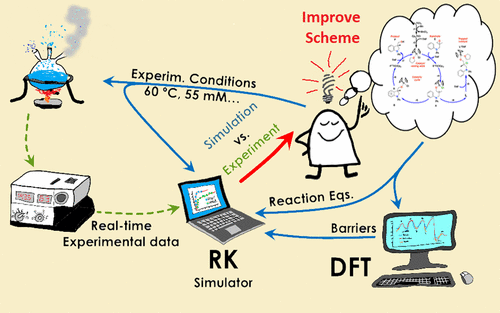
\includegraphics[height=2.55in,width=4.05in]{Figures/Schematic_Material-Design.png}
%\caption{\tiny \textrm{Pseudopotential for metallic sodium, based on the empty core model and screened by the Thomas-Fermi dielectric function.}}%(与文献\cite{EPJB33-47_2003}图1对比)
%\caption{\tiny \textrm{Pseudopotential for metallic sodium, based on the empty core model and screened by the Thomas-Fermi dielectric function.}}%(与文献\cite{EPJB33-47_2003}图1对比)
\label{Schematic_Material-Design}
\end{figure}
}

\frame
{
	\frametitle{材料模拟的基本思想和方法}
\begin{figure}[h!]
\vspace*{-0.25in}
\centering
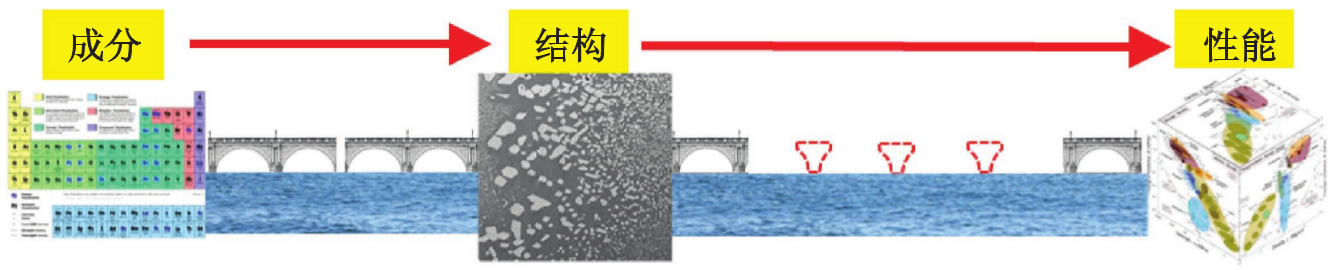
\includegraphics[height=0.80in,width=4.05in]{Figures/MGE-2.png}
%\caption{\tiny \textrm{Pseudopotential for metallic sodium, based on the empty core model and screened by the Thomas-Fermi dielectric function.}}%(与文献\cite{EPJB33-47_2003}图1对比)
\vskip 0.05pt
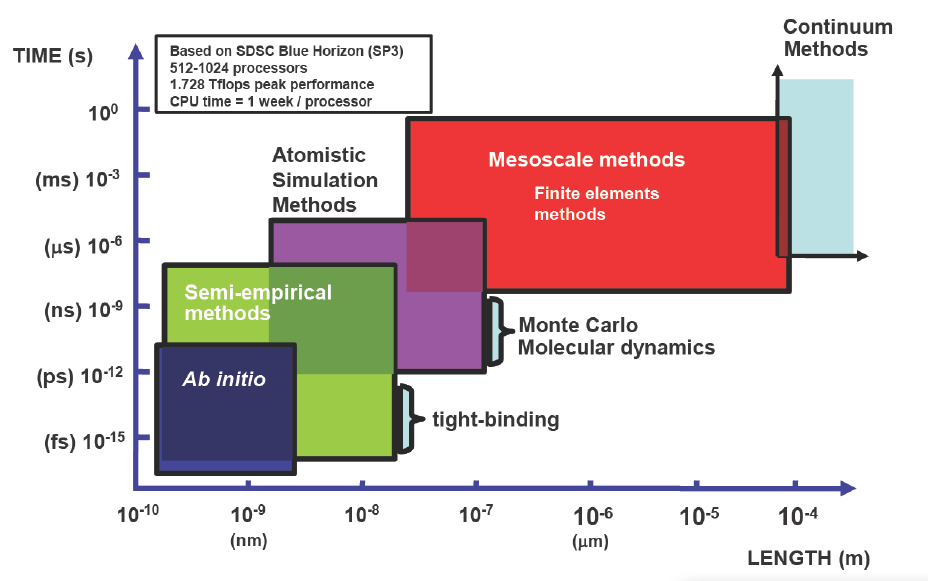
\includegraphics[height=2.20in,width=3.45in]{Figures/Multi-Scale-6.png}
%\caption{\tiny \textrm{Pseudopotential for metallic sodium, based on the empty core model and screened by the Thomas-Fermi dielectric function.}}%(与文献\cite{EPJB33-47_2003}图1对比)
\label{Multi-Scale}
\end{figure}
}

\frame
{
	\frametitle{材料计算软件发展现状}
\begin{figure}[h!]
\vspace*{-0.16in}
\centering

\includegraphics[width=3.30in]{Figures/Softwares_logo.png}
%\caption{\tiny \textrm{Pseudopotential for metallic sodium, based on the empty core model and screened by the Thomas-Fermi dielectric function.}}%(与文献\cite{EPJB33-47_2003}图1对比)
\label{Softwares}
\end{figure}
}

\frame
{
	\frametitle{国产第一原理计算软件现状}
\begin{figure}[h!]
\vspace*{-0.19in}
\centering
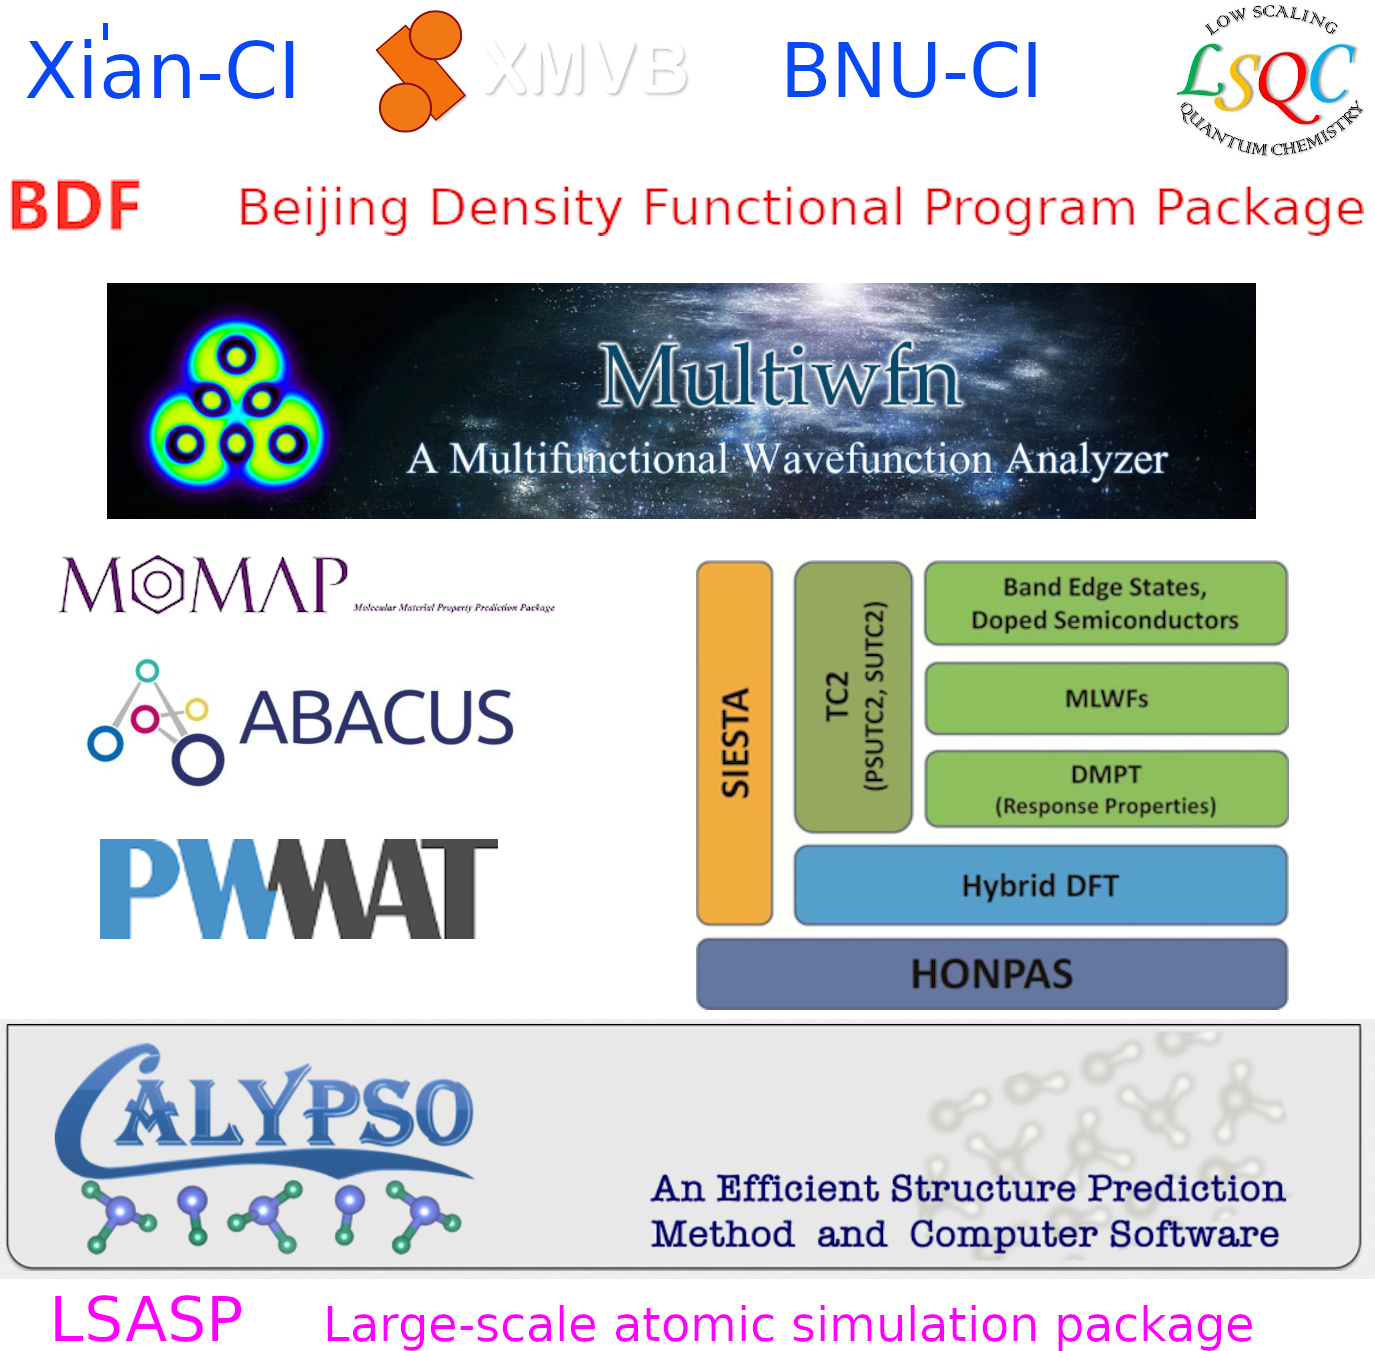
\includegraphics[width=2.83in]{Figures/Softwares_China-logo.png}
%\caption{\tiny \textrm{Pseudopotential for metallic sodium, based on the empty core model and screened by the Thomas-Fermi dielectric function.}}%(与文献\cite{EPJB33-47_2003}图1对比)
\label{Software-China}
\end{figure}
	\fontsize{6.2pt}{5.2pt}\selectfont{\textcolor{red}{中国学科发展战略\,$\cdot$\,理论与计算化学,~~国家自然科学基金委员会,~中国科学院,~~北京:~科学出版社,~~2016}}
}

\frame
{
\frametitle{\textrm{WIEN2k}软件简介}
\begin{figure}[h!]
\centering
\vspace*{-0.16in}
%\subfigure[\footnotesize{Logo of WIEN2k}]{
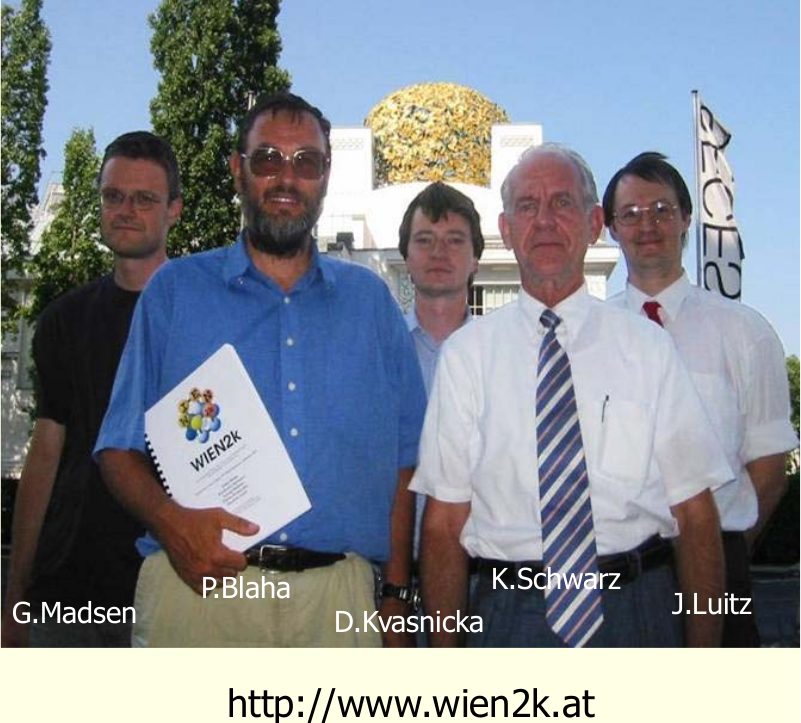
\includegraphics[height=1.5in]{Figures/WIEN2k-Group.png}
\hskip 0.5pt
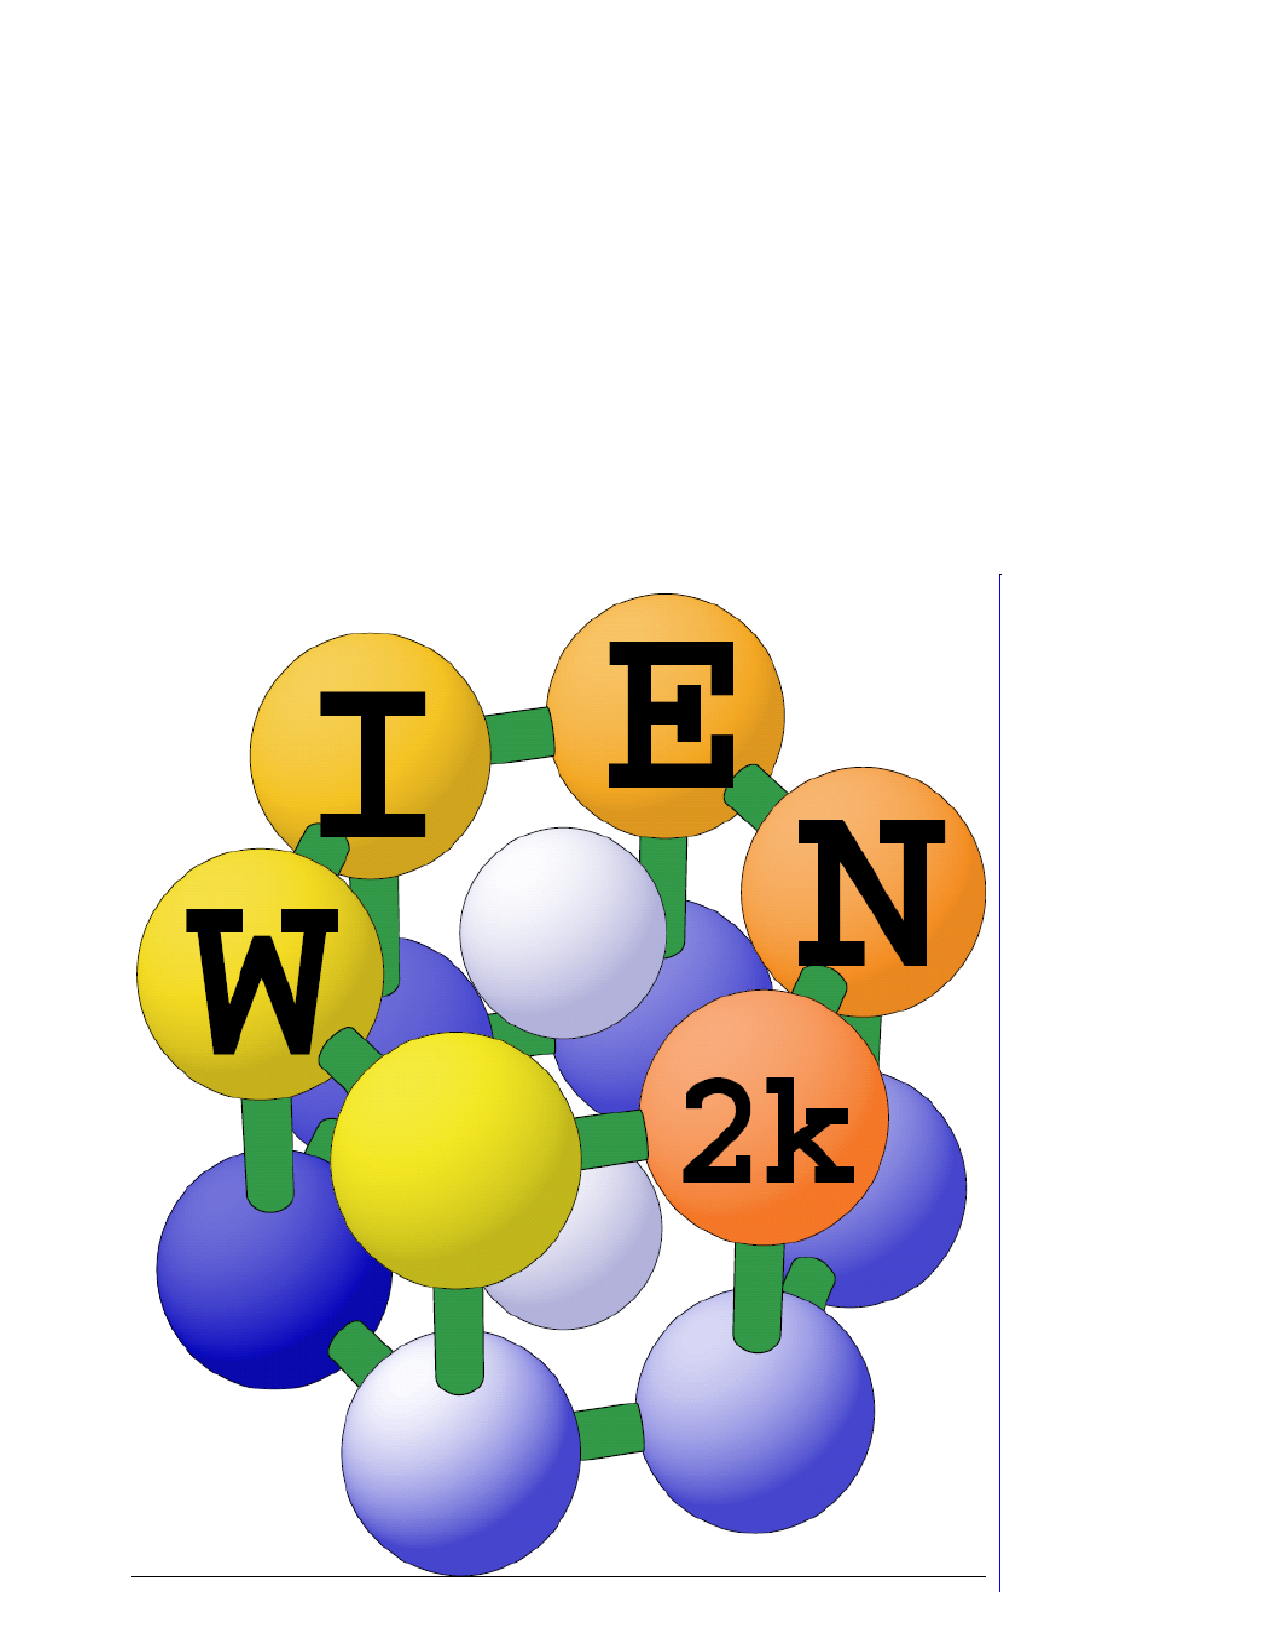
\includegraphics[height=1.5in,width=1.6in,viewport=13 35 475 515,clip]{Figures/logo_WIEN2k.pdf}
%\caption{\tiny \textrm{}}%(与文献\cite{EPJB33-47_2003}图1对比)
%\label{Brillouin_Cube}
%}
%\subfigure[\footnotesize{Logo of VASP}]{
%\includegraphics[height=1.48in,width=2.24in,viewport=55 145 595 455,clip]{logo_VASP.eps}
%\caption{\tiny \textrm{}}%(与文献\cite{EPJB33-47_2003}图1对比)
\label{Logo_of_WIEN2k}
%}
\end{figure}
\textrm{WIEN2k}是由奥地利维也纳技术大学\textrm{(Vienna University of Technology)}开发的高精度第一原理材料计算软件包\upcite{WIEN2k_UG}。%\\\textrm{WIEN2k};\textrm{VASP}。
\begin{itemize}
	\item 采用普适的全势\textrm{(Full-Potential, FP)}方法\\对计算对象的化学环境依赖小
	\item \textrm{LAPW}基组\\兼备描述波函数邻近原子核和位于原子核间行为的能力
	\item 计算精度高,结果常作为理论计算的\textrm{Benchmark}
%	\item \textrm{VASP}:采用\textrm{USPP-PAW}方法,计算效率高,特别擅长计算材料的力学性质\upcite{VASP_UG}
\end{itemize}
}

\frame
{
	\frametitle{\textrm{WIEN2k}软件简介}
\begin{minipage}[t]{0.55\textwidth}
	制约\textrm{WIEN2k}软件应用的主要因素
	\begin{itemize}
		\item 高精度计算必须付出的代价\\
			\textcolor{blue}{计算速度慢,处理体系有限}
		\item 各计算模块部分独立\\
			\textcolor{red}{输入控制文件过多}\\
			\textcolor{red}{输出数据文件分散}
		\item 采用\textrm{tcsh}脚本串联各部分\\
			计算中间结果需写入外部存储\\
			\textcolor{red}{\textrm{I/O}耗时过多}
		\item 软件的并行环境设置拙劣\\
			\textcolor{red}{\textrm{mpi}并行效率低下}
		\item \textcolor{red}{编译安装繁琐}
	\end{itemize}
\end{minipage}
\hfill
\begin{minipage}[t]{0.43\textwidth}
\begin{figure}[h!]
\centering
\vspace*{-10pt}
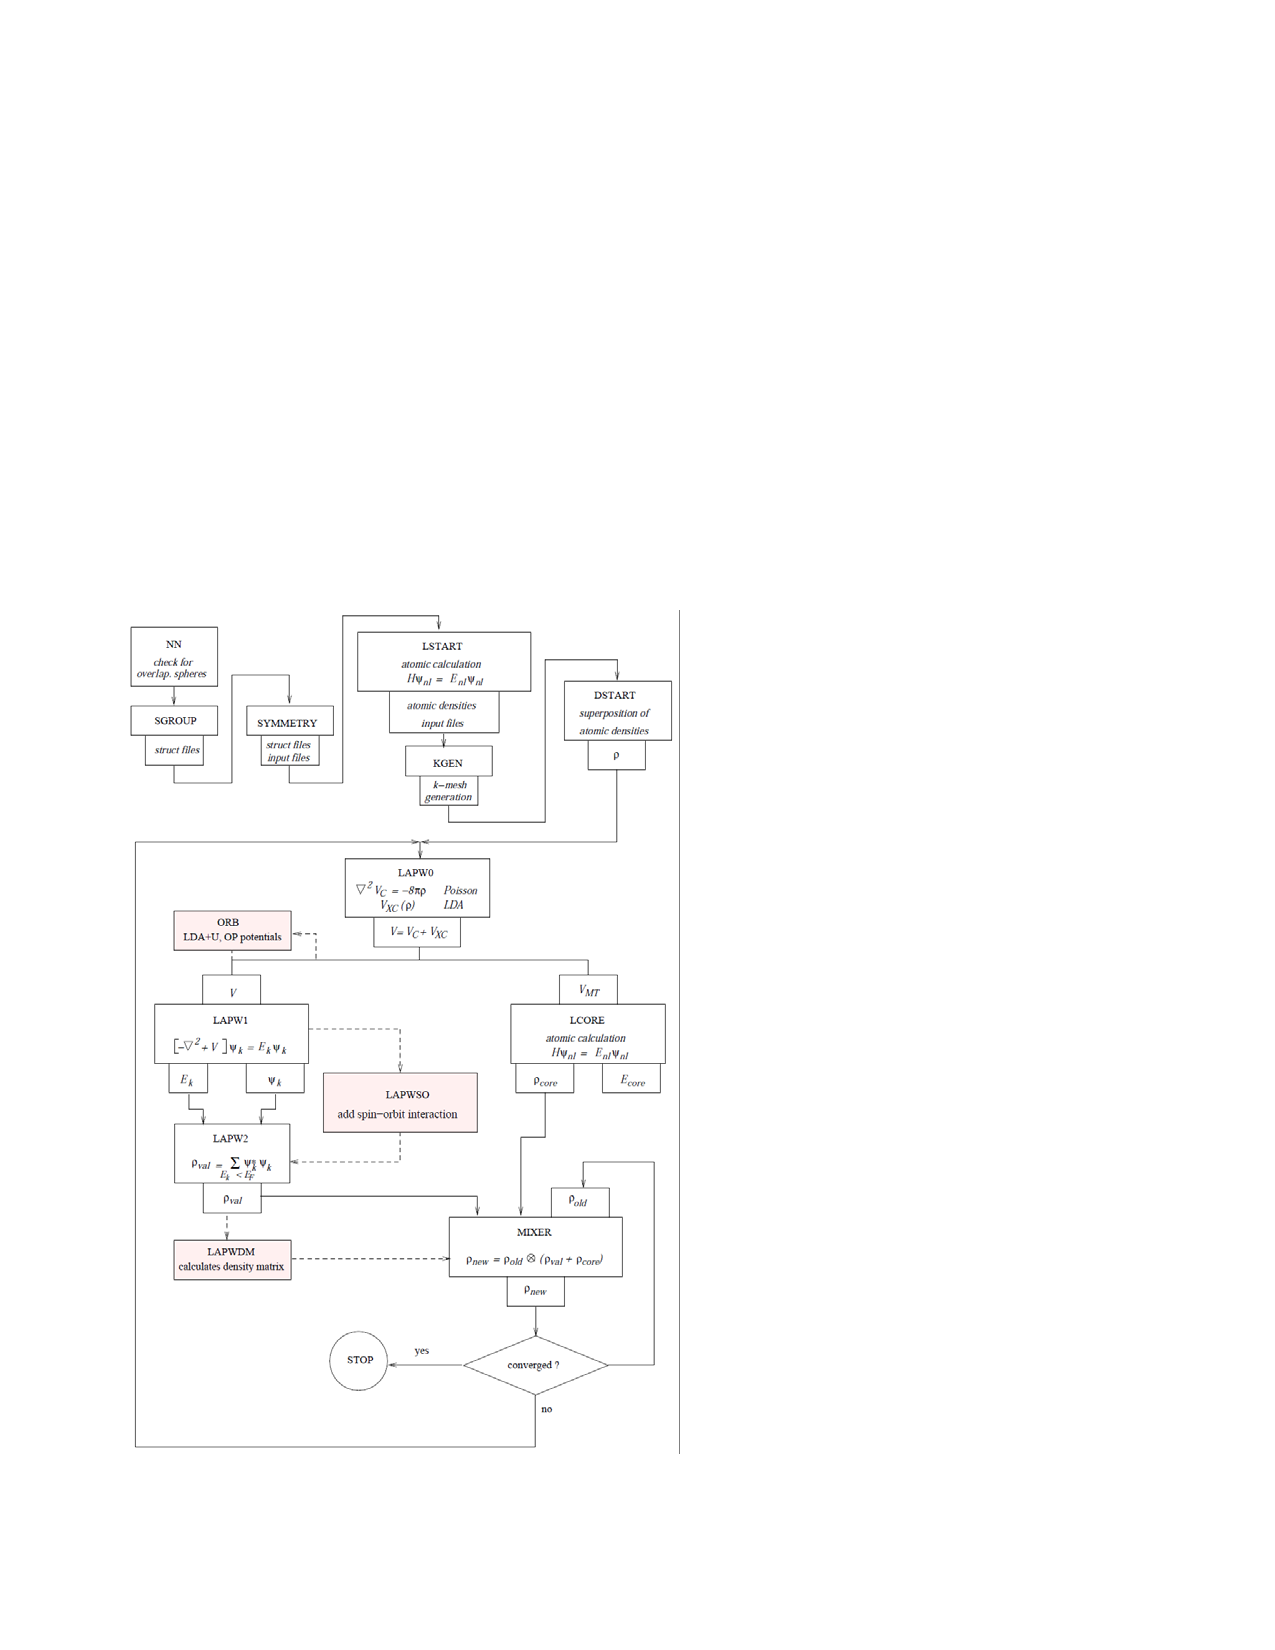
\includegraphics[height=2.6in,width=1.60in,viewport=60 90 325 500,clip]{Figures/WIEN2k_Program_flow.pdf}
\caption{\tiny \textrm{Program flow in WIEN2k.}}%(与文献\cite{EPJB33-47_2003}图1对比)
\label{WIEN2k_program_flow}
\end{figure}
\end{minipage}
}

%-----------------------------------------------------------------------------------------------------------------------------------------------------------------------%
\section{量子力学基础}
\subsection{能量量子化}
\frame
{
	\frametitle{经典物理学的成功}
\begin{figure}[h!]
\vspace*{-0.18in}
\centering
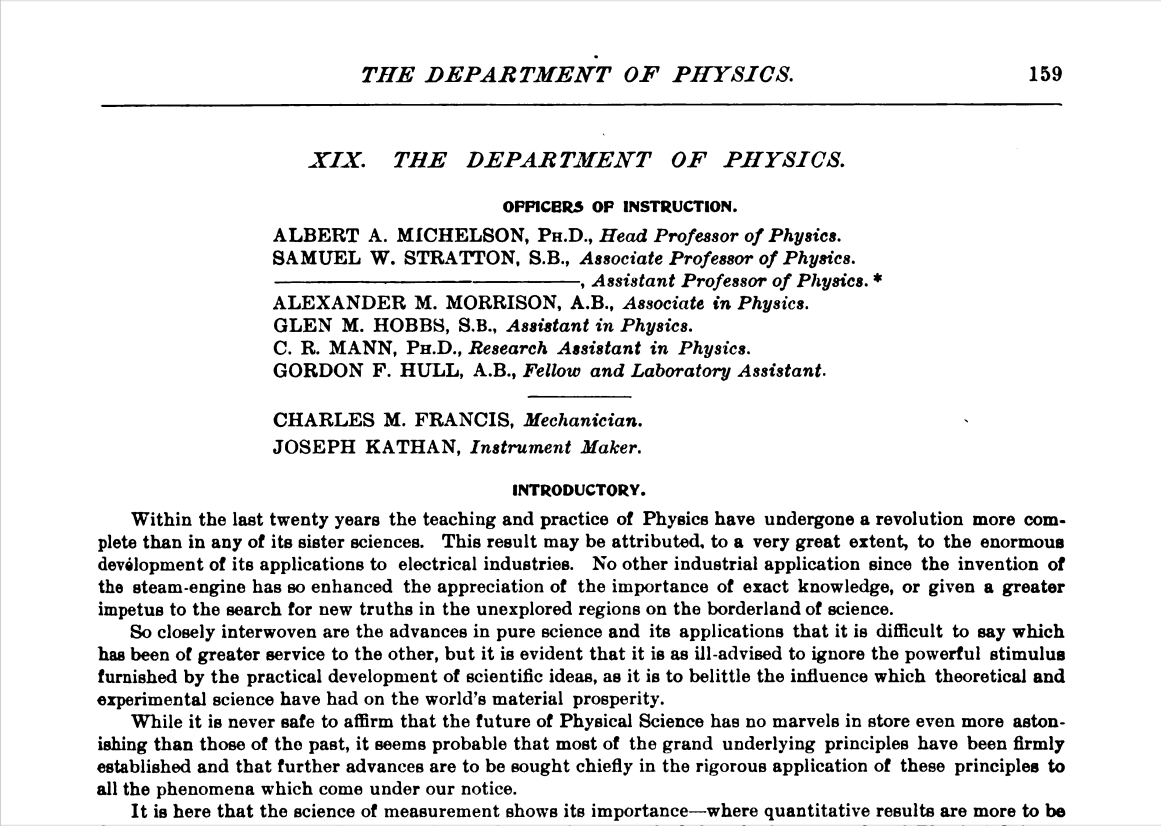
\includegraphics[height=1.90in,width=3.00in,viewport=0 0 1150 690,clip]{Figures/Albert_Michelson-Quotes.jpg}
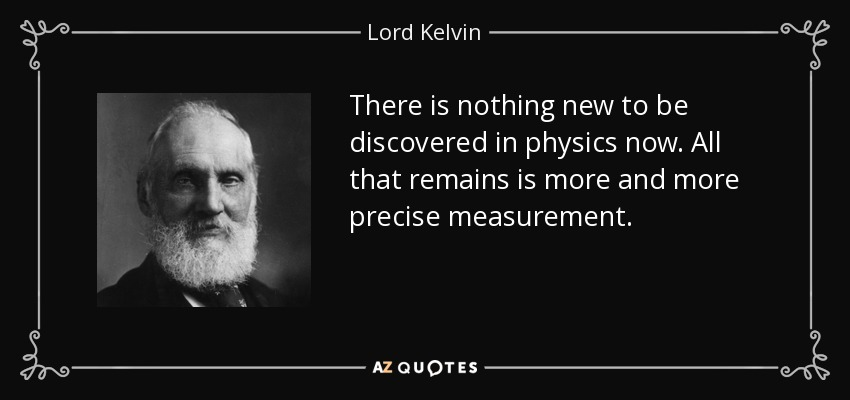
\includegraphics[height=1.10in,width=2.55in,viewport=0 0 880 400,clip]{Figures/Quote-there-is-nothing-new-to-be-discovered-in-physics-now-all-that-remains-is-more-and-more-lord-kelvin-57-38-79.jpg}
%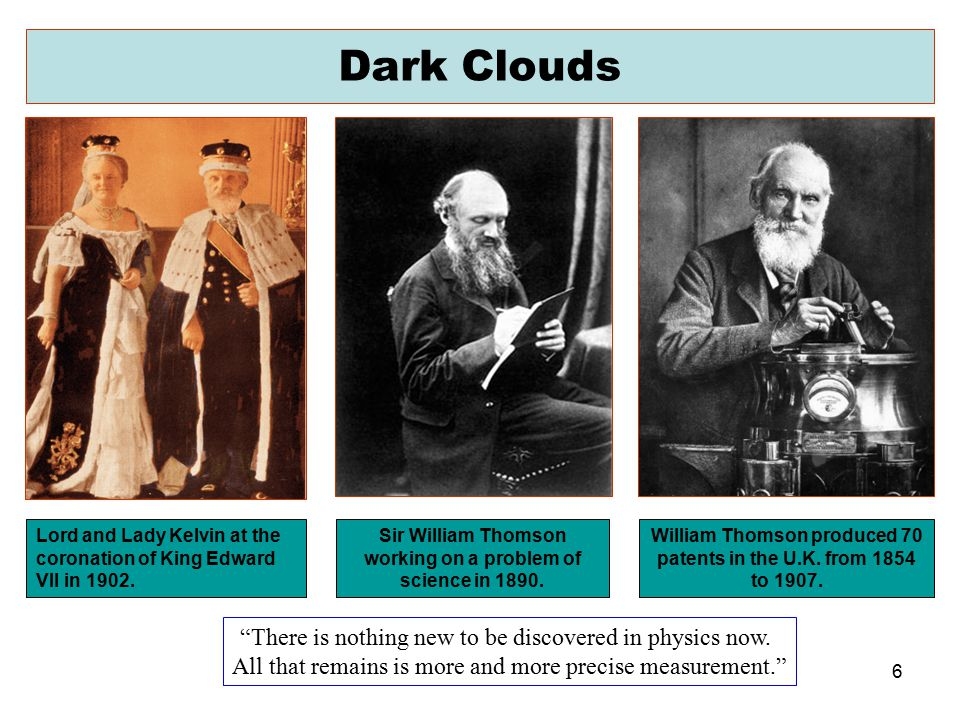
\includegraphics[height=2.50in,width=4.05in,viewport=0 20 735 470,clip]{Figures/Two-dark-cloud-in-physics-3.jpg}
%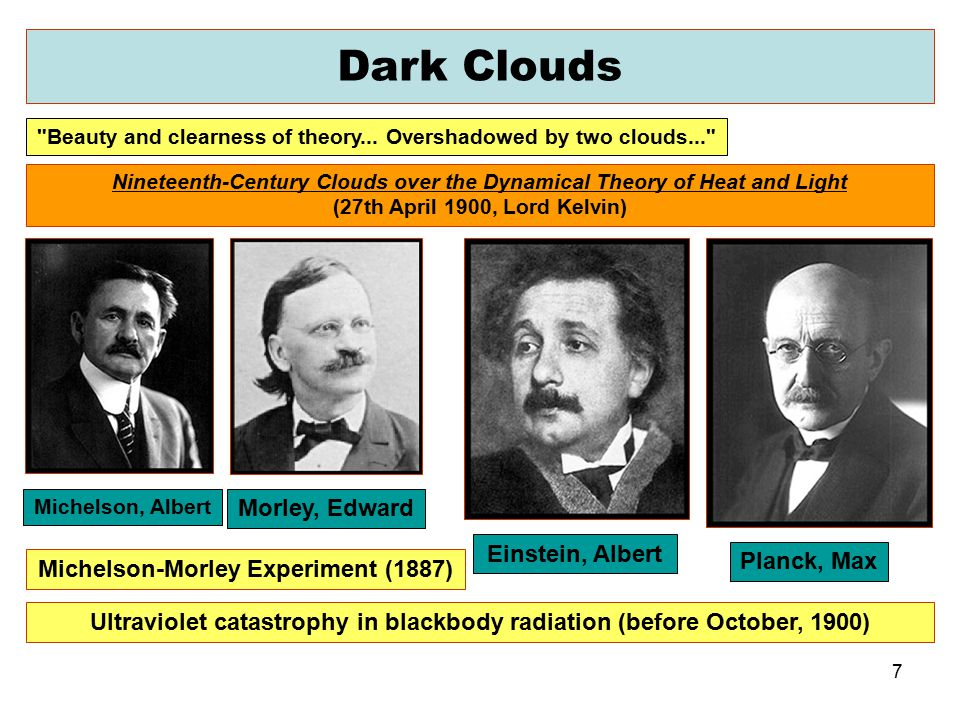
\includegraphics[height=2.40in,width=4.05in,viewport=0 50 735 470,clip]{Figures/Two-dark-cloud-in-physics-2.jpg}
%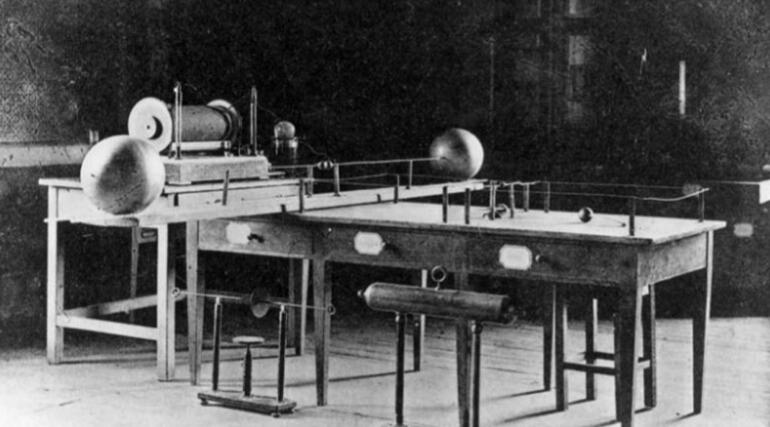
\includegraphics[height=2.40in,width=4.05in,viewport=0 0 580 325,clip]{Figures/Two-dark-cloud-in-physics-1.jpg}
\label{two_Dark_Clouds}
\end{figure}
}

\frame
{
	\frametitle{经典物理学天空的“两朵乌云”\textrm{(Dark Clouds)}}
\begin{figure}[h!]
\vspace*{-0.18in}
\centering
%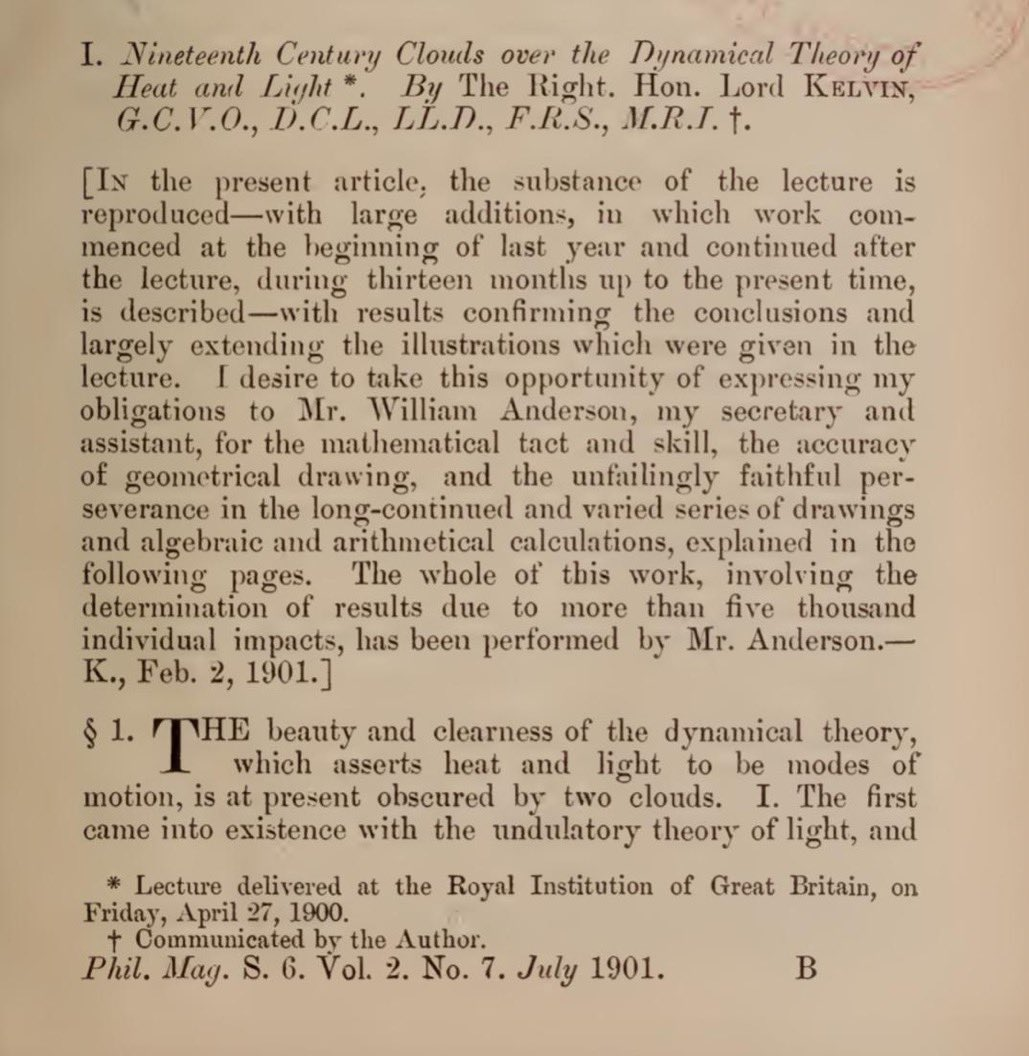
\includegraphics[height=2.90in,width=2.80in,viewport=0 0 1000 1100,clip]{Figures/Baron_Kelvin-Lecture.jpeg}
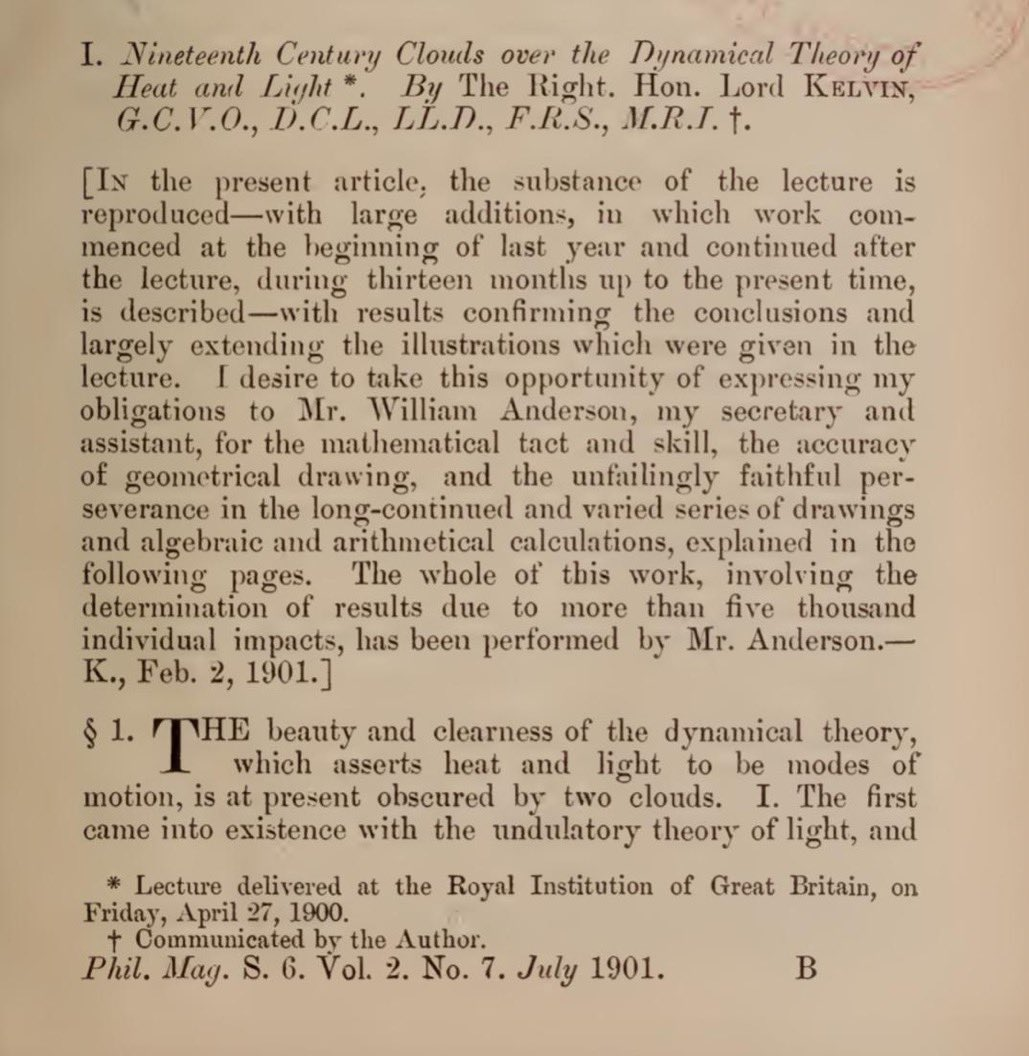
\includegraphics[height=0.35in,width=3.35in,viewport=0 900 1020 1030,clip]{Figures/Baron_Kelvin-Lecture.jpeg}
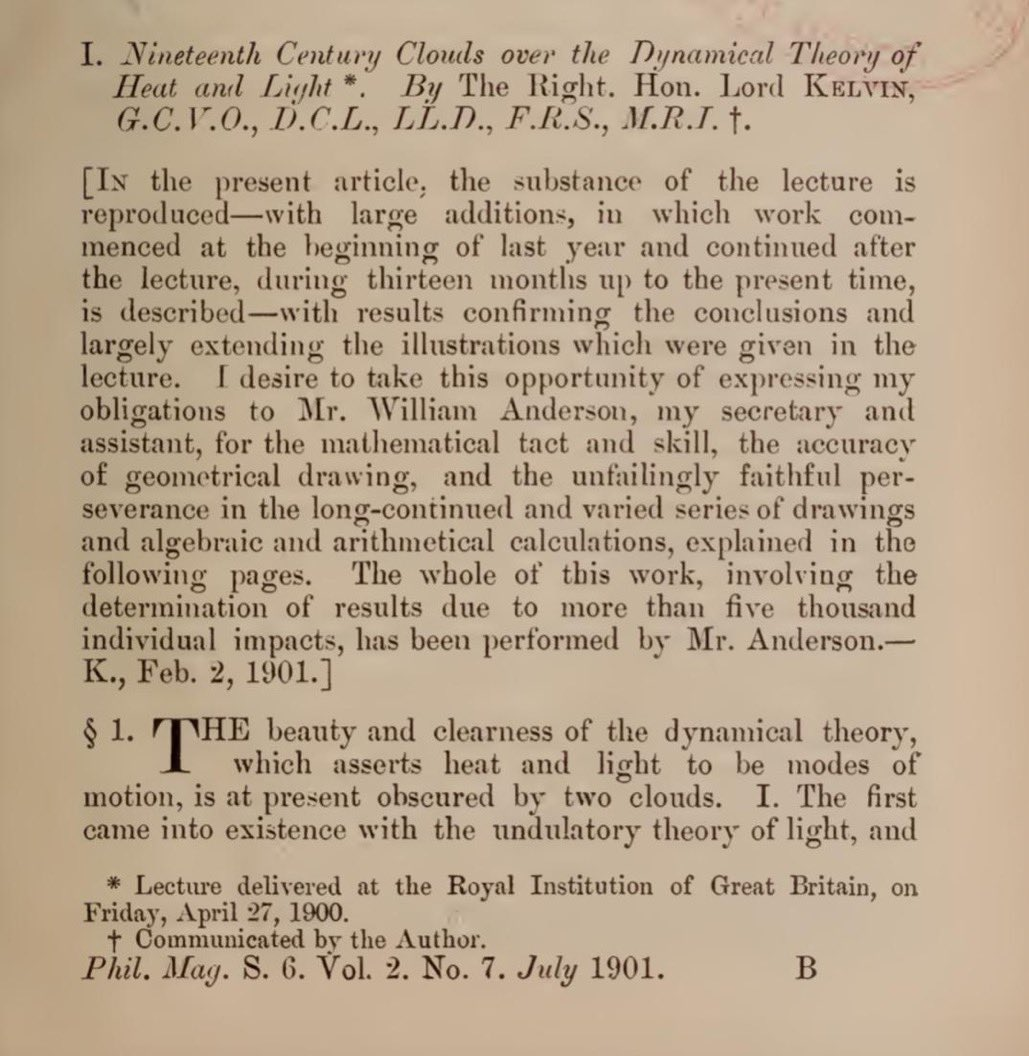
\includegraphics[height=0.80in,width=3.35in,viewport=0 50 1020 350,clip]{Figures/Baron_Kelvin-Lecture.jpeg}
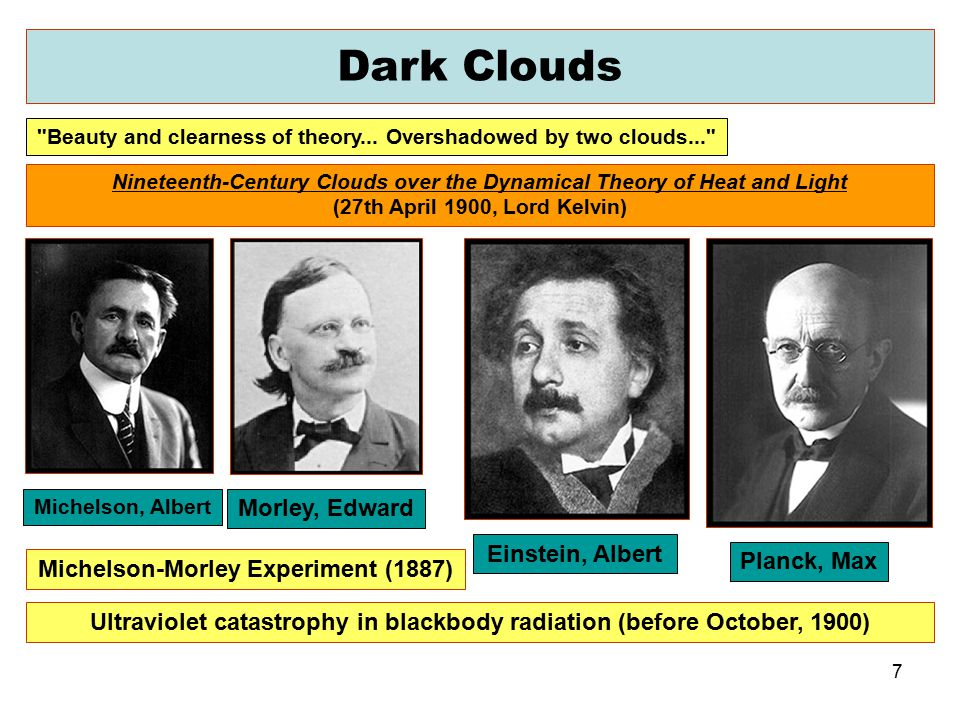
\includegraphics[height=1.85in,width=4.05in,viewport=0 50 735 370,clip]{Figures/Two-dark-cloud-in-physics-2.jpg}
\label{two_Dark_Clouds_2}
\end{figure}
}

%\frame
%{
%	\frametitle{经典物理学天空的“两朵乌云”\textrm{(Dark Clouds)}}
%\begin{figure}[h!]
%\vspace*{-0.18in}
%\centering
%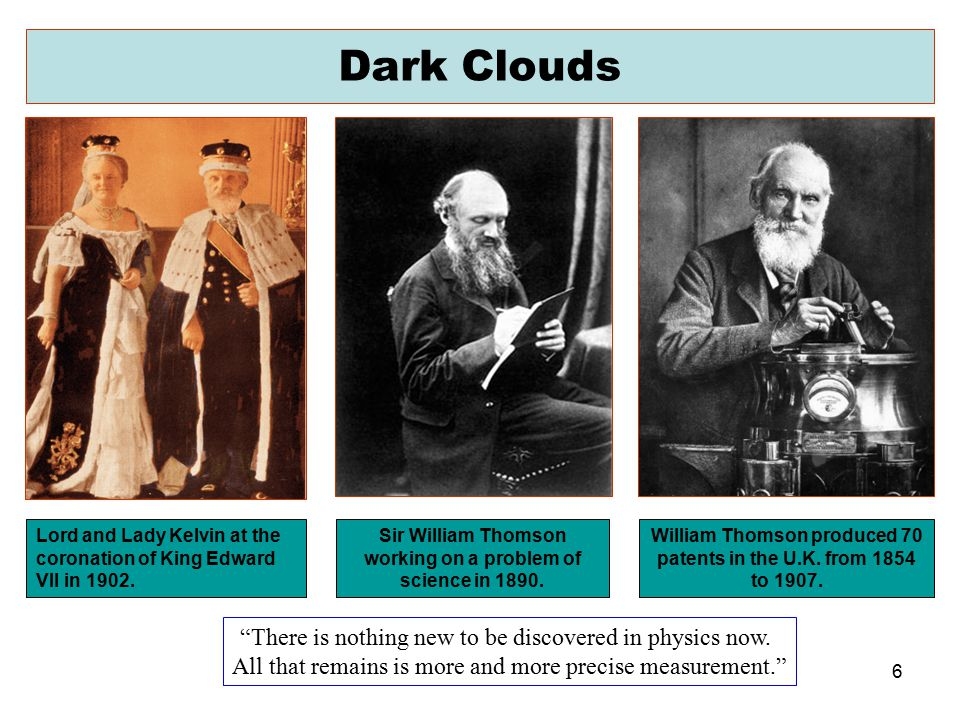
\includegraphics[height=2.50in,width=4.05in,viewport=0 20 735 470,clip]{Figures/Two-dark-cloud-in-physics-3.jpg}
%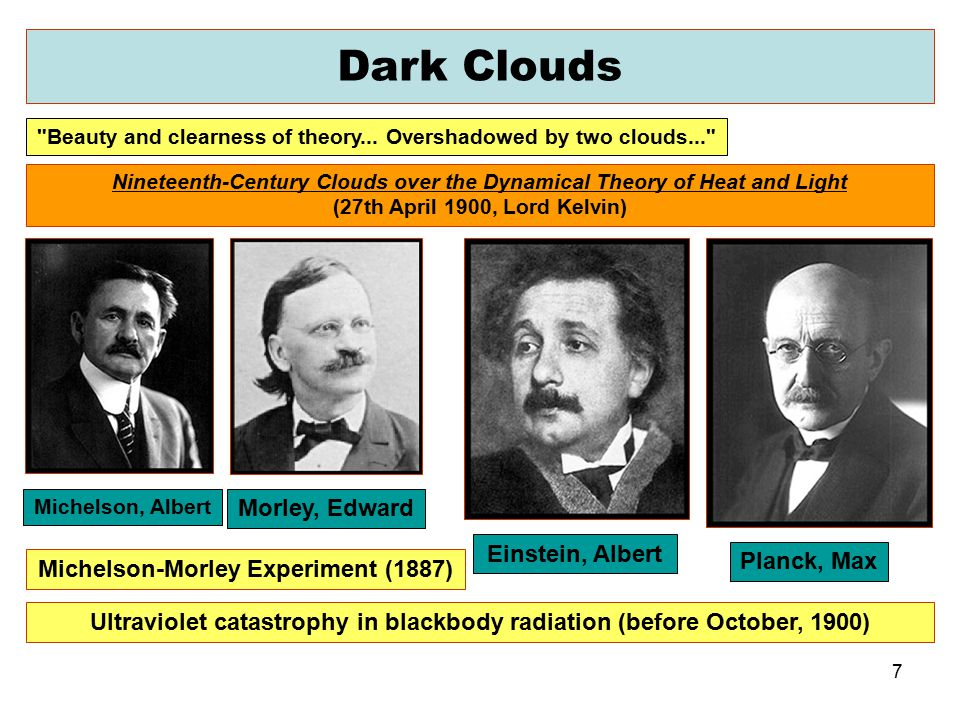
\includegraphics[height=2.40in,width=4.05in,viewport=0 50 735 470,clip]{Figures/Two-dark-cloud-in-physics-2.jpg}
%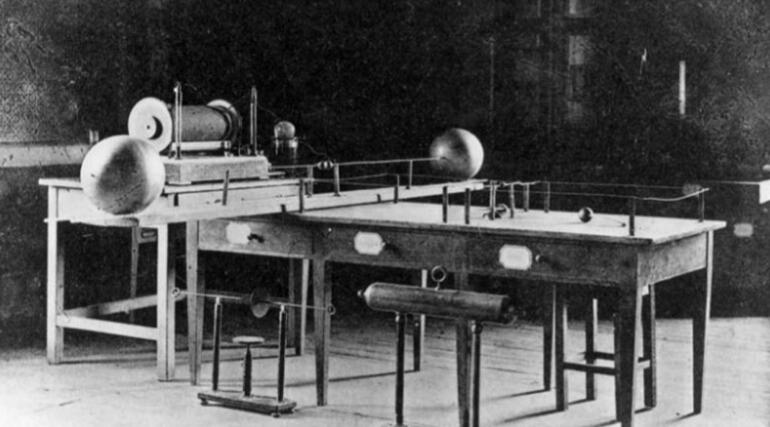
\includegraphics[height=2.40in,width=4.05in,viewport=0 0 580 325,clip]{Figures/Two-dark-cloud-in-physics-1.jpg}
%\label{two_Dark_Clouds_3}
%\end{figure}
%}
%
\frame
{
	\frametitle{黑体辐射与能量量子化}
	\textrm{1900}年,为了解释黑体辐射\textrm{(black-body radiation)}的能量密度与电磁辐射频率的关系,\textrm{M.~Planck}%放弃\textcolor{blue}{能量均分定理}\textrm{(the equipartition theorem)},
	引入\textcolor{red}{能量量子化}\textrm{(quantization of energy)}的假设,利用统计物理推导出与实验符合得非常好的黑体辐射\textrm{Planck~}公式:~
	\begin{displaymath}
		\rho_{\nu}\mathrm{d}{\nu}=\dfrac{8{\pi}h{\nu}^3}{C^2}\bigg(\dfrac1{\mathrm{e}^{h\nu/kT}-1}\bigg)\mathrm{d}\nu
	\end{displaymath}
\begin{figure}[h!]
\centering
\vspace{-10.5pt}
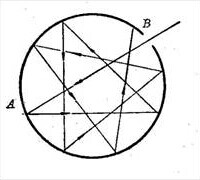
\includegraphics[height=1.45in,width=1.45in,viewport=0 0 136 136,clip]{Figures/Black_box.jpg}
\hskip 1pt
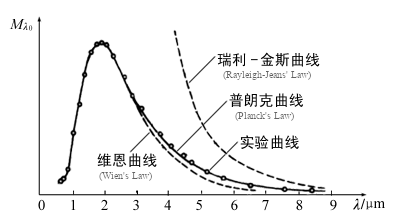
\includegraphics[height=1.32in,width=2.25in,viewport=0 0 390 215,clip]{Figures/Black_box_curve.png}
\caption{\textrm{The black-body radiation and the curve}}
\label{Black_box}
\end{figure}
}

\frame
{
	\frametitle{波-粒二象性与光电效应}
\begin{figure}[h!]
\centering
\vspace{-15.5pt}
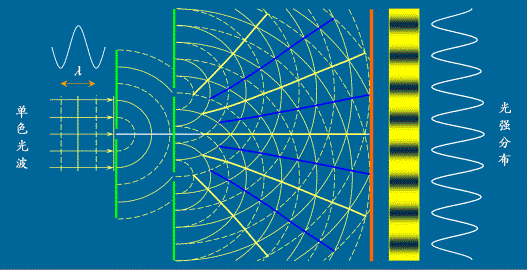
\includegraphics[height=1.35in,width=2.70in,viewport=0 0 536 280,clip]{Figures/wave-particle_duality.png}
\vskip 1pt
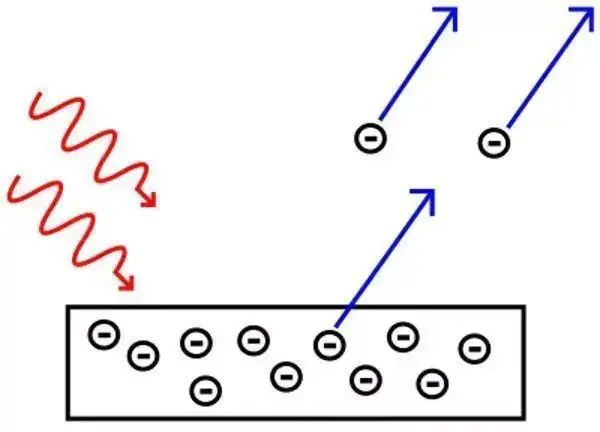
\includegraphics[height=1.32in,width=2.05in,viewport=0 0 620 455,clip]{Figures/Photoelectic_effect.png}
\caption{\textrm{The wave-particle duality and Photoelectric effect}}
\label{wave_and_particle}
\end{figure}
}

\frame
{
	\frametitle{电子衍射、\textrm{Compton~effect}与\textrm{H}原子光谱}
\begin{figure}[h!]
\centering
\vspace{-15.5pt}
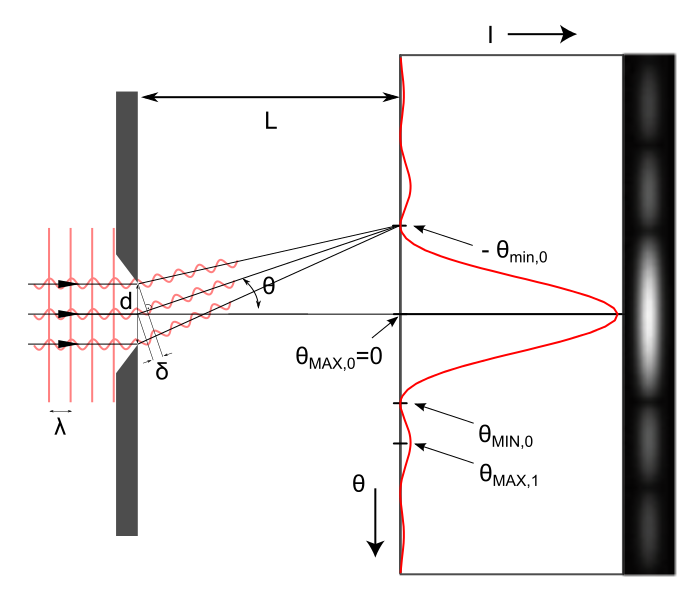
\includegraphics[height=1.35in,width=1.80in,viewport=0 0 680 600,clip]{Figures/Single_Slit_Diffraction.png}
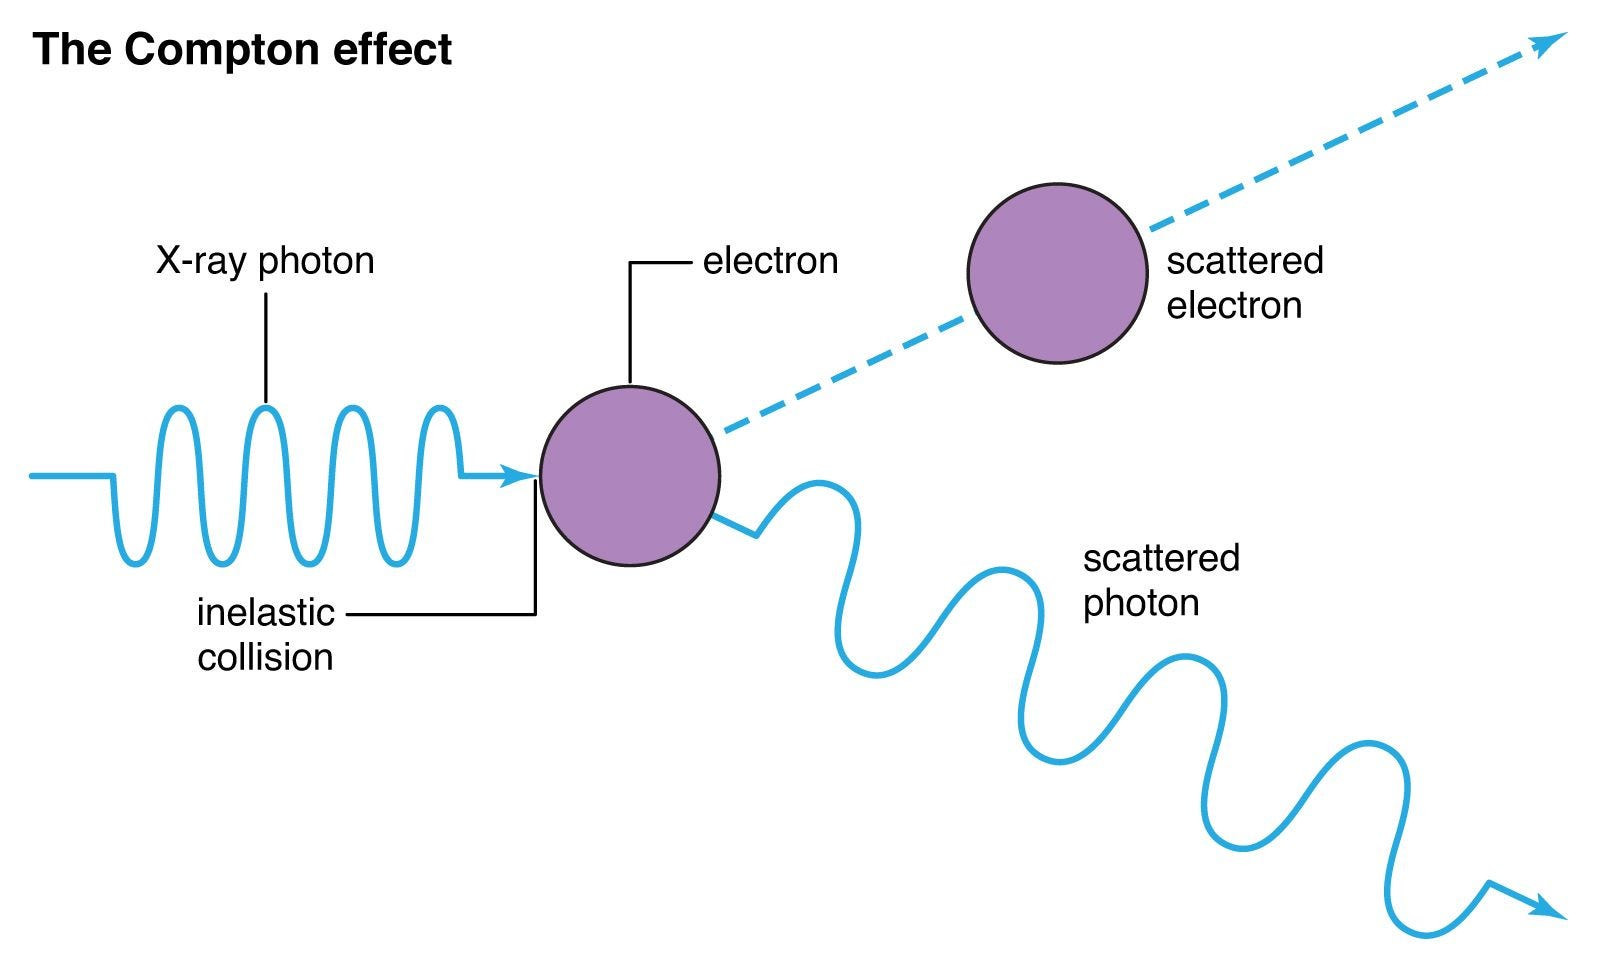
\includegraphics[height=1.20in,width=2.10in,viewport=0 0 1600 950,clip]{Figures/Compton_effect.jpg}\\
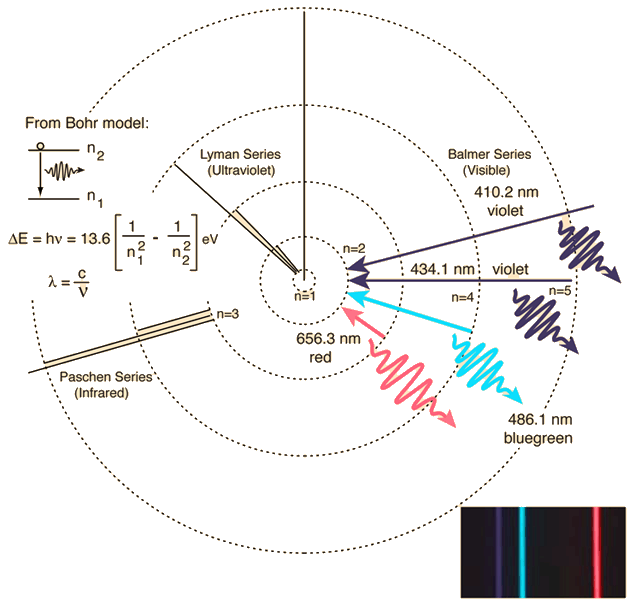
\includegraphics[height=1.65in,width=1.75in,viewport=0 0 620 600,clip]{Figures/Hydrogen_spectrum-3.png}
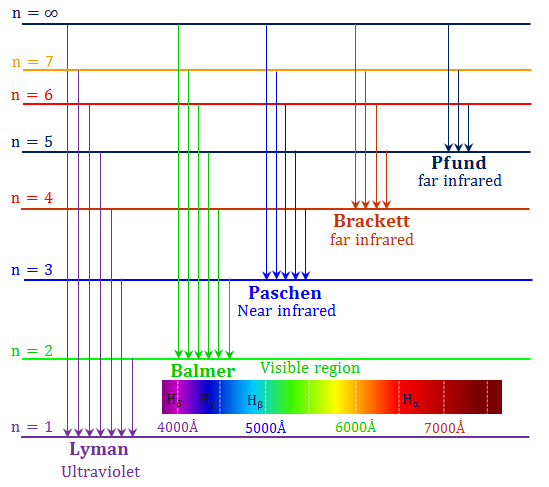
\includegraphics[height=1.55in,width=1.75in,viewport=0 0 500 380,clip]{Figures/Hydrogen_spectrum-2.png}
%\caption{\textrm{The wave-particle duality and Photoelectric effect}}
\label{electron:wave_and_particle}
\end{figure}
}

\subsection{\textrm{Schr\"odinger}方程与量子力学的建立}
\frame
{
	\frametitle{\textrm{De Broglie}物质波}
\begin{minipage}{0.53\textwidth}
\begin{figure}[h!]
\centering
\vspace{-15.5pt}
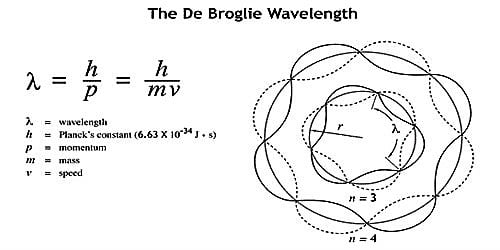
\includegraphics[height=1.3in,width=2.1in,viewport=0 0 500 280,clip]{Figures/De-Broglie-waves.jpg}
%\caption{\textrm{The wave-particle duality and Photoelectric effect}}
\label{Matter_wave}
\end{figure}
经典的观念:
\begin{itemize}
	\item \textcolor{red}{粒子}:~\textcolor{blue}{物质存在的形式}
	\item \textcolor{red}{波动}:~\textcolor{blue}{能量传递的形式}
\end{itemize}
\end{minipage}
\begin{minipage}{0.45\textwidth}
\begin{figure}[h!]
\centering
\vspace{-15.5pt}
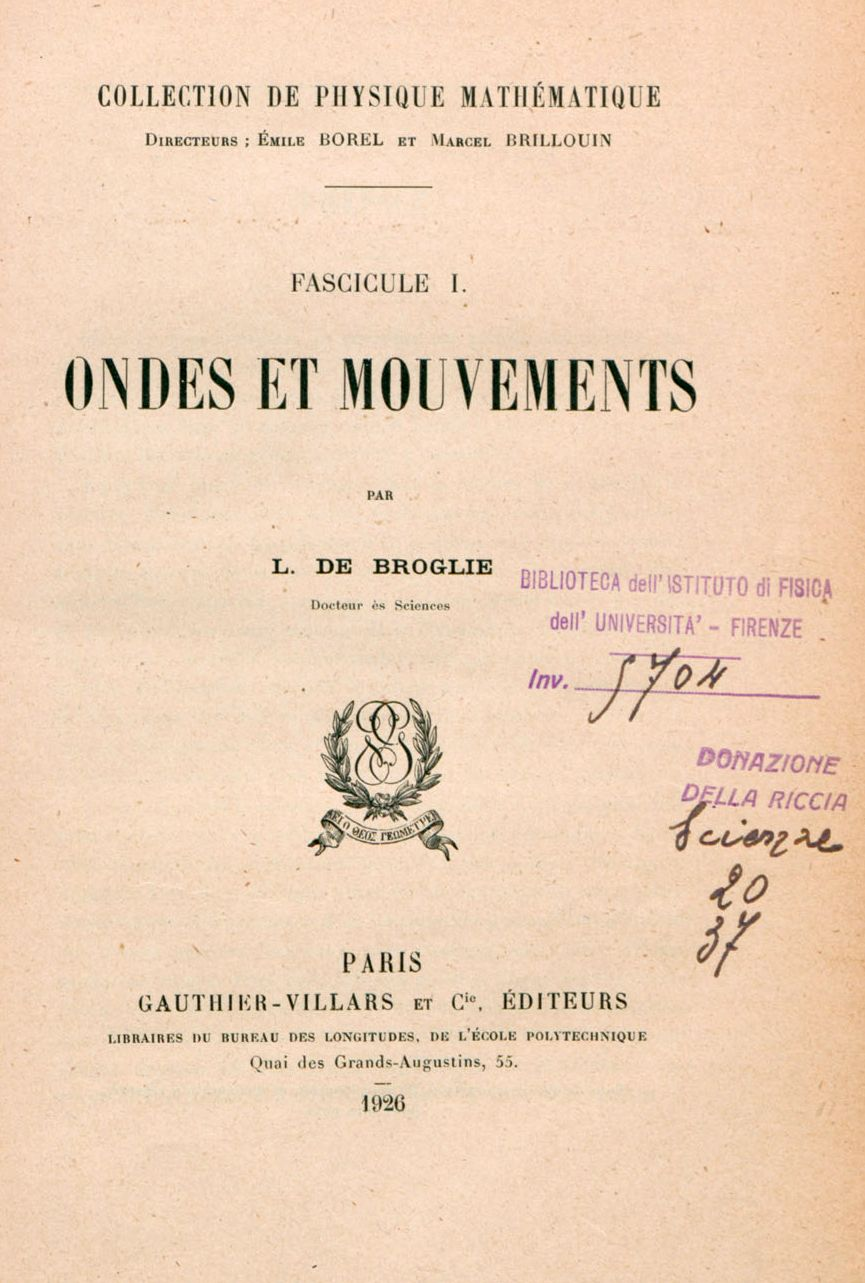
\includegraphics[height=2.80in,width=1.90in,viewport=0 0 430 650,clip]{Figures/De_Broglie-dissertation_Cover.jpg}
%\caption{\textrm{The wave-particle duality and Photoelectric effect}}
\label{De_Broglie-dissertation}
\end{figure}
\end{minipage}
}

\frame
{
	\frametitle{经典力学\textrm{Classical Mechanics}}
\begin{figure}[h!]
\vspace*{-0.18in}
\centering
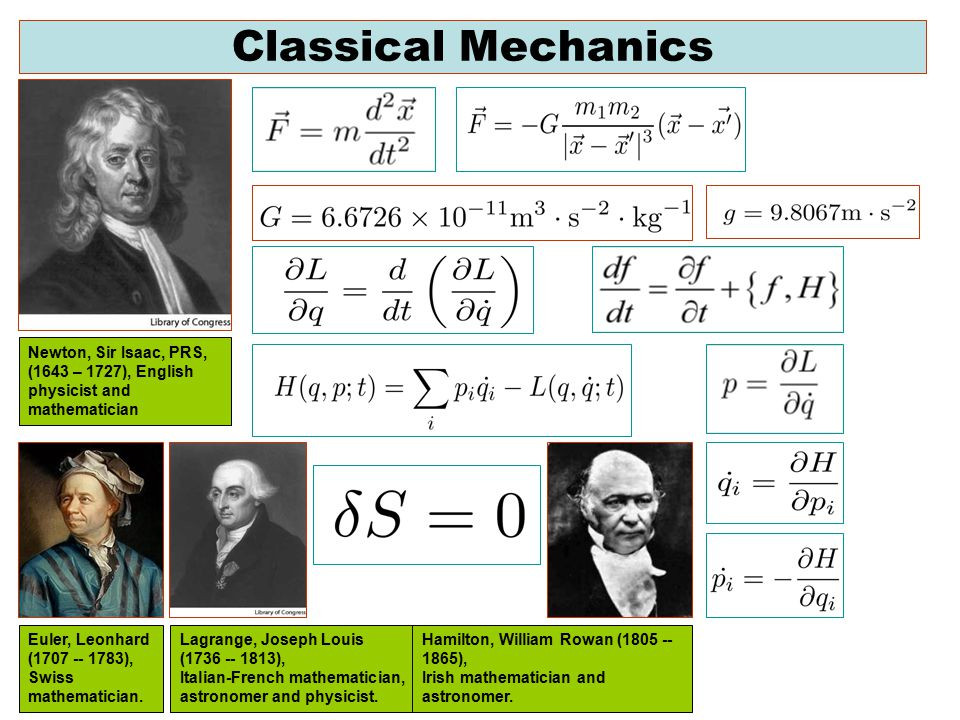
\includegraphics[height=2.65in,width=4.05in,viewport=0 0 715 495,clip]{Figures/Classical_Mechanics.jpg}
%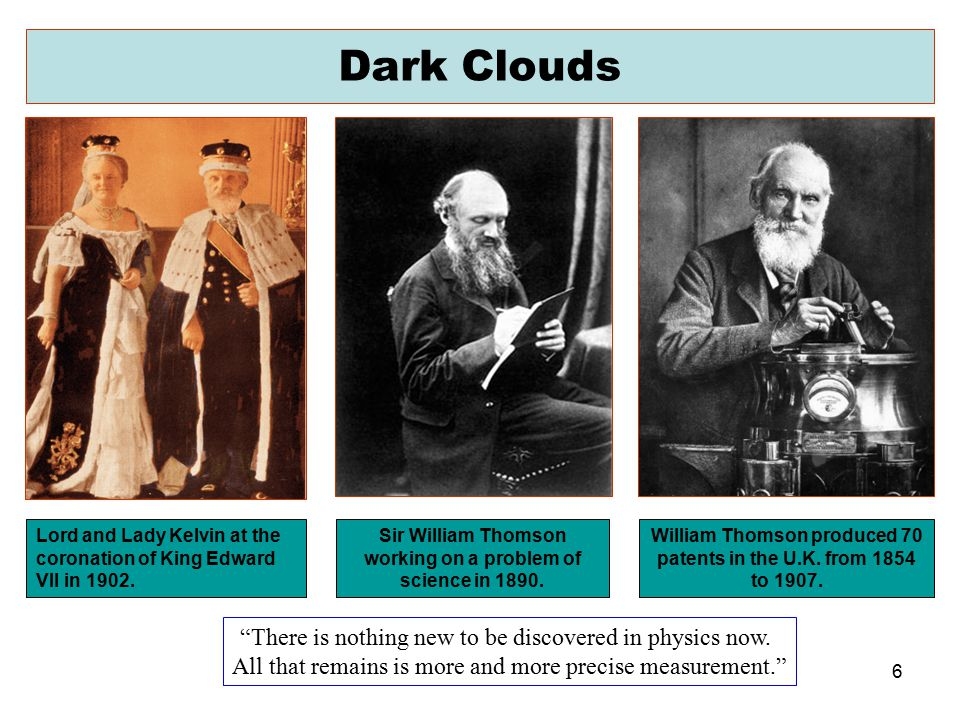
\includegraphics[height=2.50in,width=4.05in,viewport=0 20 735 470,clip]{Figures/Two-dark-cloud-in-physics-3.jpg}
%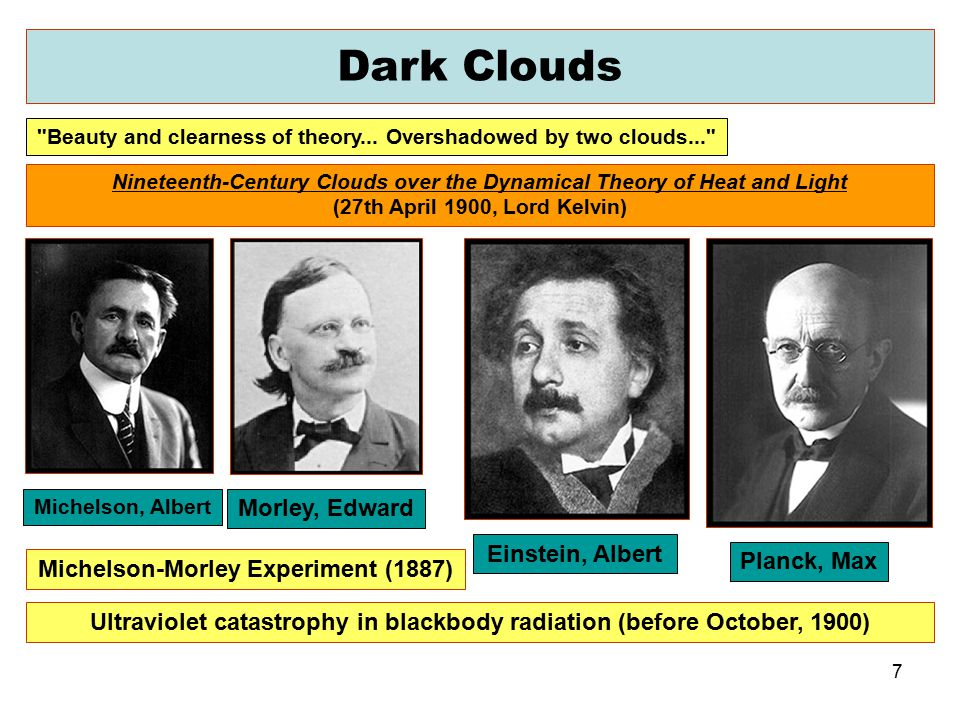
\includegraphics[height=2.40in,width=4.05in,viewport=0 50 735 470,clip]{Figures/Two-dark-cloud-in-physics-2.jpg}
%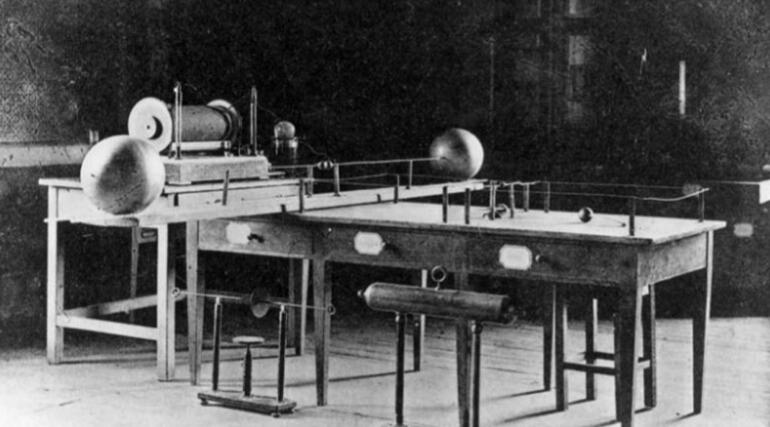
\includegraphics[height=2.40in,width=4.05in,viewport=0 0 580 325,clip]{Figures/Two-dark-cloud-in-physics-1.jpg}
\label{Classical_Mechanics}
\end{figure}
}

\frame
{
	\frametitle{\textrm{\small Newtonian, Lagrangian and Hamiltonian Mechanics}}
	\begin{itemize}
   		\setlength{\itemsep}{10pt}
		\item \textrm{\textcolor{blue}{Newtonian~Mechanics}}\\
		牛顿运动定律体系是以力、加速度、动量这些矢量为基本量来描述力学系统在欧氏空间的运动~(用几何方程表述约束)
	\item \textrm{\textcolor{blue}{Lagrangian~Mechanics}}\\
		拉格朗日力学是关于研究对象在其对应的约束系统下的运动形式,大大压缩牛顿方程描述需要的约束个数。不需要在另外设未知数目
	\item \textrm{\textcolor{blue}{Hamiltonian~Mechanics}}\\
		哈密度力学由拉格朗日力学演变而来,把位置和动量彻底分开,成为两种独立变量,由此诞生相空间。把广义动量和广义坐标放在等同的位置上(正则配对,方程降阶)
		\vskip 6pt
		拉格朗日力学和哈密顿力学的基本量是\textcolor{blue}{系统的能量}等标量,通过变分原理建立系统的动力学方程,所以拉格朗日力学和哈密顿力学合称\textcolor{magenta}{分析力学}
	\end{itemize}
}

\frame
{
	\frametitle{\textrm{Invariante Variationsprobleme}}
\begin{figure}[h!]
\centering
%
\vspace{-10.5pt}
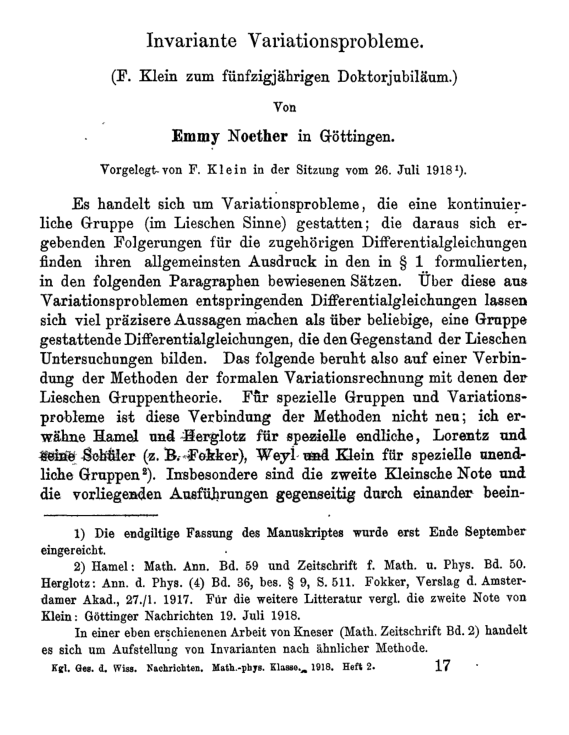
\includegraphics[height=0.52\textwidth,width=0.42\textwidth,viewport=0 0 450 580,clip]{Figures/Noether_theorem-1st_page.png}
\label{Noether_theorem}
\end{figure}
\begin{itemize}
\centering
	\item \textcolor{red}{能量守恒}~$\Longleftrightarrow$~\textcolor{magenta}{时间平移对称性}
	\item \textcolor{red}{动量守恒}~$\Longleftrightarrow$~\textcolor{magenta}{空间平移对称性}
	\item \textcolor{red}{角动量守恒}~$\Longleftrightarrow$~\textcolor{magenta}{空间旋转对称性}
\end{itemize}
}

\frame
{
	\frametitle{\textrm{驻波}}
\begin{figure}[h!]
\centering
\vspace{-15.5pt}
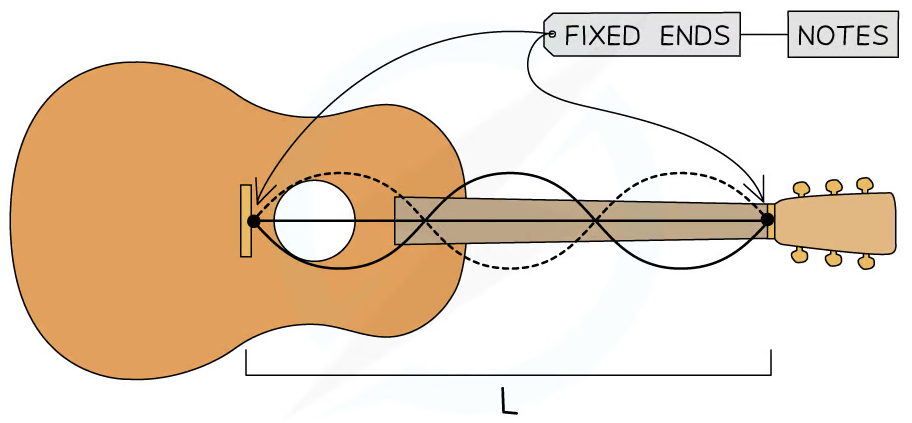
\includegraphics[height=0.40\textwidth,width=0.8\textwidth,viewport=0 0 900 450,clip]{Figures/Guitar-string.png}
\vskip 0.1pt
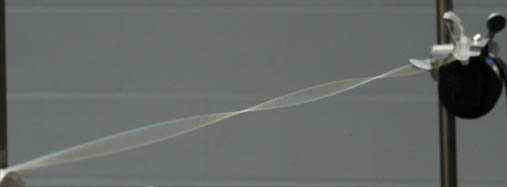
\includegraphics[height=0.35\textwidth,width=0.8\textwidth,viewport=0 0 122 48,clip]{Figures/string-standing-wave.jpg}
%\caption{\textrm{ABINIT}的Si.in}
\label{Standing_Wave_0}
\end{figure}
}

\frame
{
	\frametitle{驻波方程与势阱}
\begin{figure}[h!]
\centering
\vspace{-12.5pt}
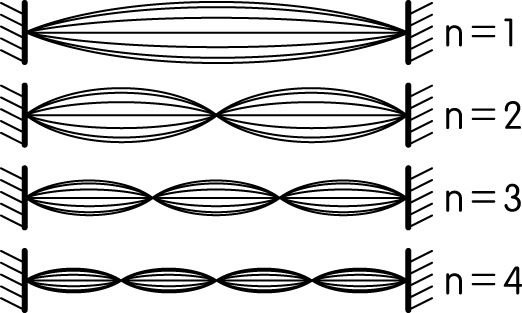
\includegraphics[height=0.32\textwidth,width=0.7\textwidth,viewport=0 0 125 75,clip]{Figures/Standing_wave.jpeg}
\vskip 2pt
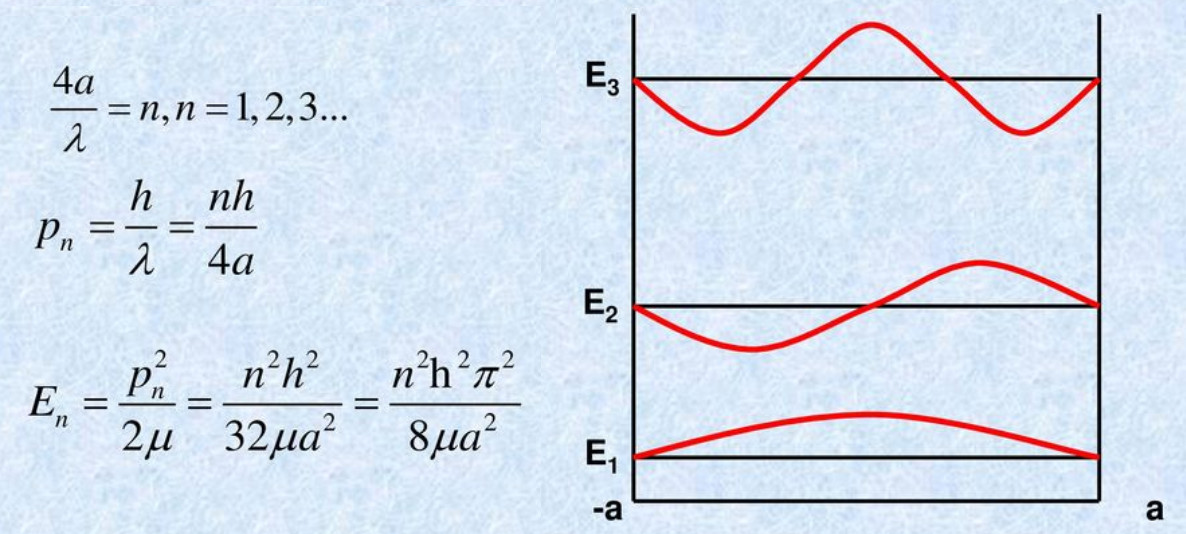
\includegraphics[height=0.40\textwidth,width=0.9\textwidth,viewport=0 0 1200 550,clip]{Figures/Standing_wave-energy.jpg}
%\caption{\textrm{ABINIT}的Si.in}
\label{Standing_Wave_1}
\end{figure}
}

\frame
{
	\frametitle{驻波方程与势阱}
\begin{figure}[h!]
\centering
\vspace{-5.5pt}
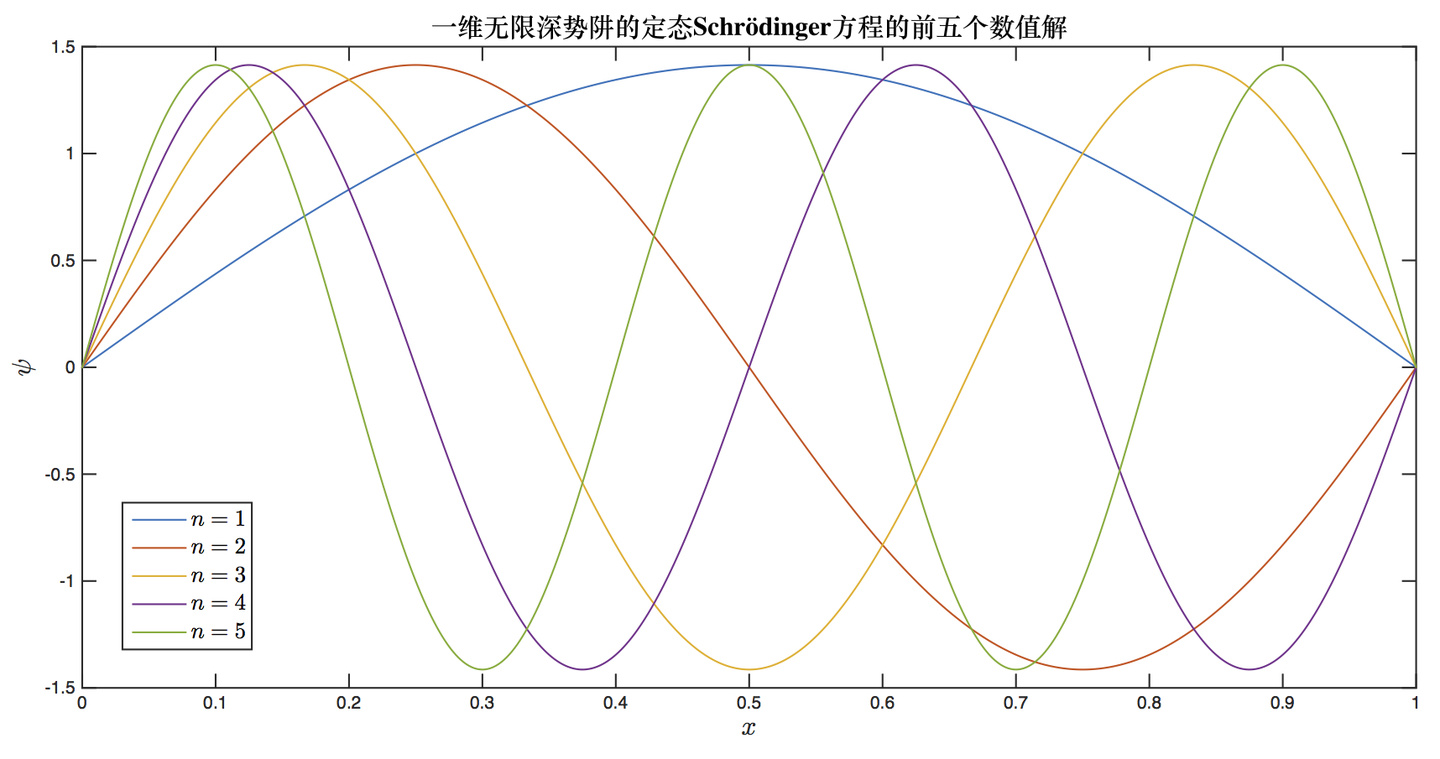
\includegraphics[height=0.55\textwidth,width=1.0\textwidth,viewport=0 0 720 400,clip]{Figures/Standing_wave-energy_1-5.jpg}
%\caption{\textrm{ABINIT}的Si.in}
\label{Standing_Wave_2}
\end{figure}
}

\frame
{
	\frametitle{驻波方程与势阱}
\begin{figure}[h!]
\centering
\vspace{-0.5pt}
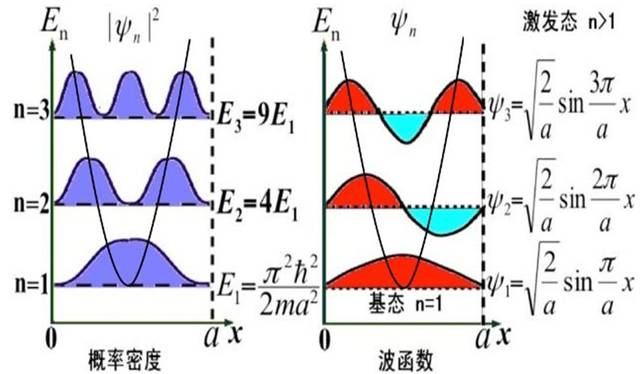
\includegraphics[height=0.46\textwidth,width=1.0\textwidth,viewport=0 0 650 390,clip]{Figures/Standing_wave_Energy.jpeg}
%\caption{\textrm{ABINIT}的Si.in}
\label{Standing_Wave_3}
\end{figure}
}

\frame
{
	\frametitle{原子中电子的驻波方程}
\begin{figure}[h!]
	\vspace{-10.5pt}
\centering
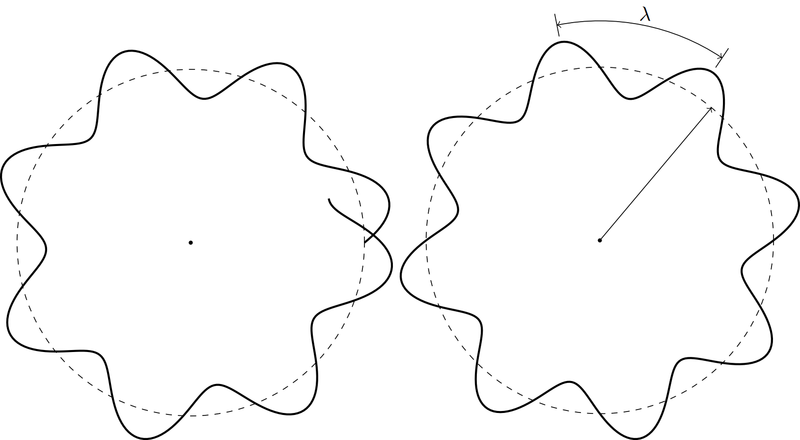
\includegraphics[height=0.38\textwidth,width=0.74\textwidth,viewport=0 0 840 440,clip]{Figures/Standing_wave-atom.png}
\vskip 2pt
\animategraphics[autoplay, loop, height=1.3in]{1}{Figures/Standing_wave_circle_}{1}{25}
\label{Atomic-electron_Standing_wave}
\end{figure}
}

\frame
{
	\frametitle{原子中的电子轨道和能量}
\begin{minipage}{0.43\textwidth}
\begin{figure}[h!]
%	\vspace{-14.8pt}
	\vspace{-4.8pt}
\centering
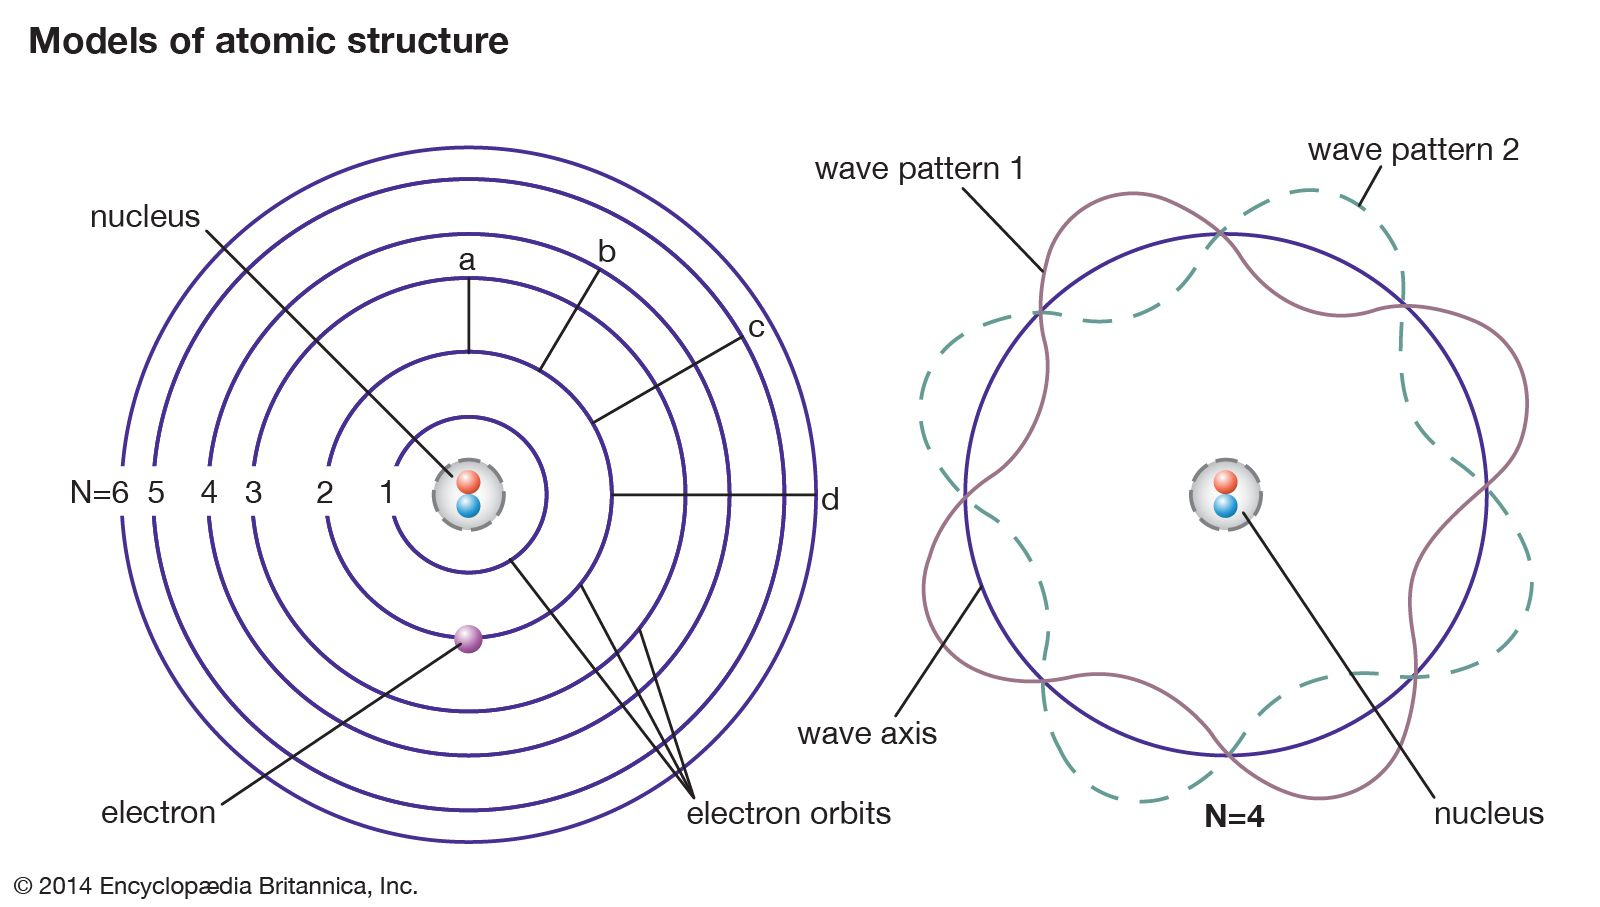
\includegraphics[height=0.57\textwidth,width=1.00\textwidth,viewport=0 50 1680 1000,clip]{Figures/electron-theory-Bohr-point-mass-energy-levels.jpg}
%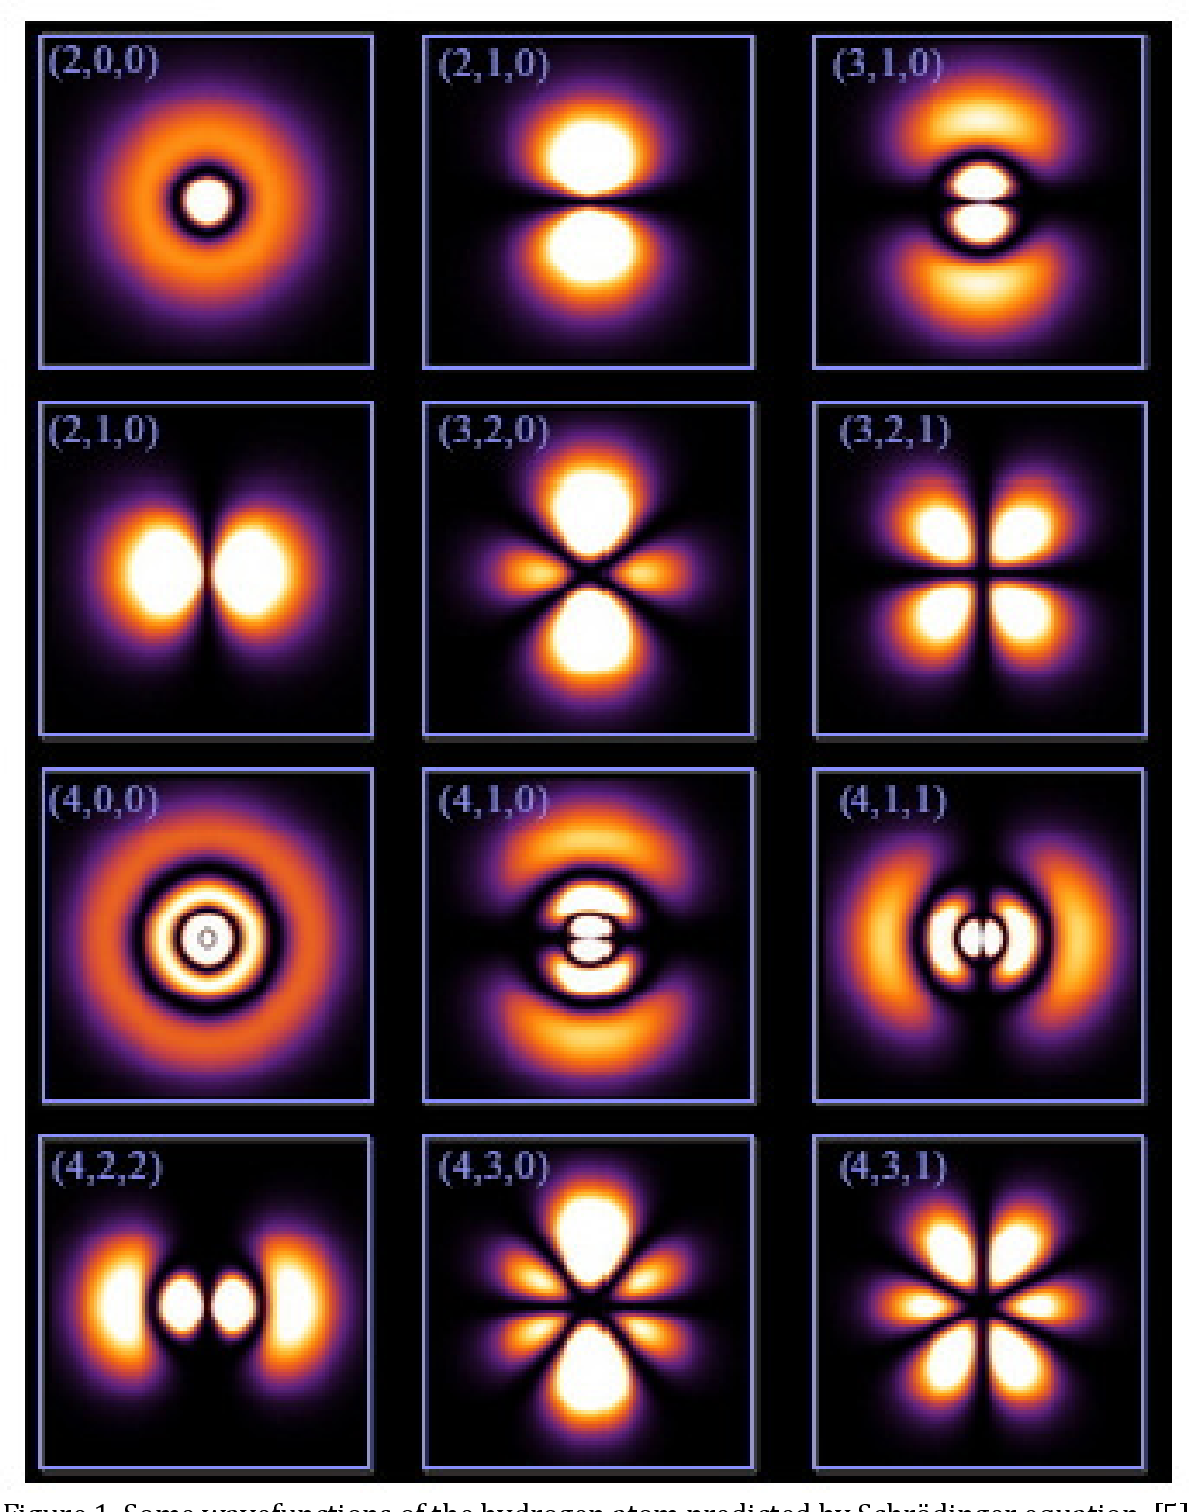
\includegraphics[height=1.23\textwidth,width=1.00\textwidth,viewport=0 10 1250 1500,clip]{Figures/wave_function.png}
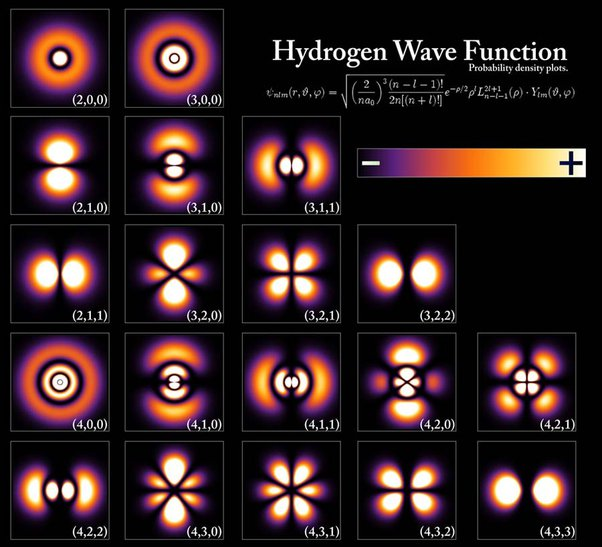
\includegraphics[height=0.95\textwidth,width=1.00\textwidth,viewport=0 0 630 650,clip]{Figures/wave_function-2.jpeg}
\label{Atomic-electron_wave}
\end{figure}
\end{minipage}
\begin{minipage}{0.55\textwidth}
\begin{figure}[h!]
	\vspace{-16.5pt}
\centering
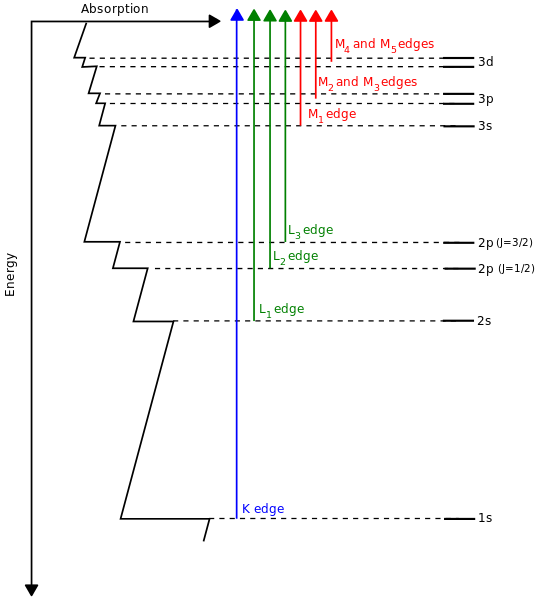
\includegraphics[height=1.10\textwidth,width=1.00\textwidth,viewport=0 0 560 600,clip]{Figures/Electron_orbital-energy.png}
\label{Atomic-electron_wave-energy}
\end{figure}
\end{minipage}
}

\frame
{
	\frametitle{\textrm{Schr\"odinger}~方程}
\begin{minipage}{0.49\textwidth}
\begin{figure}[h!]
\centering
%
\vspace{-25.5pt}
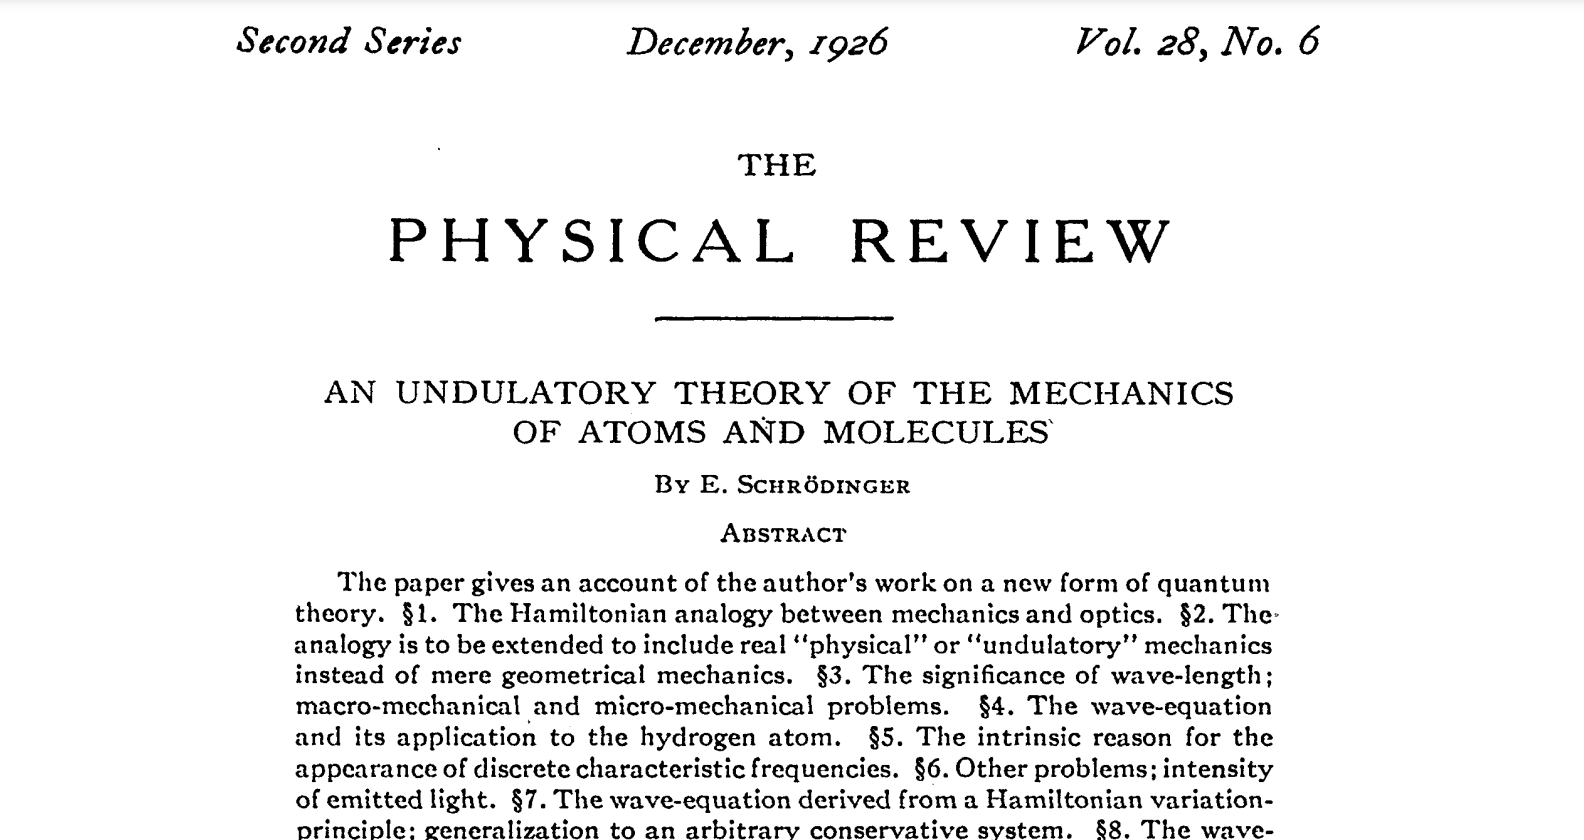
\includegraphics[height=1.80in,width=2.00in,viewport=180 0 1380 1100,clip]{Figures/Schrodinger_article.png}
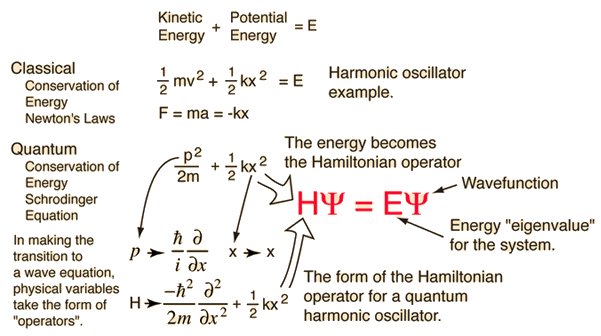
\includegraphics[height=1.20in,width=2.00in,viewport=0 0 600 350,clip]{Figures/Schrodinger_Equation.png}
\label{Schrodinger_Equation}
\end{figure}
\end{minipage}
\begin{minipage}{0.49\textwidth}
\begin{figure}[h!]
\centering
%
\vspace{-15.5pt}
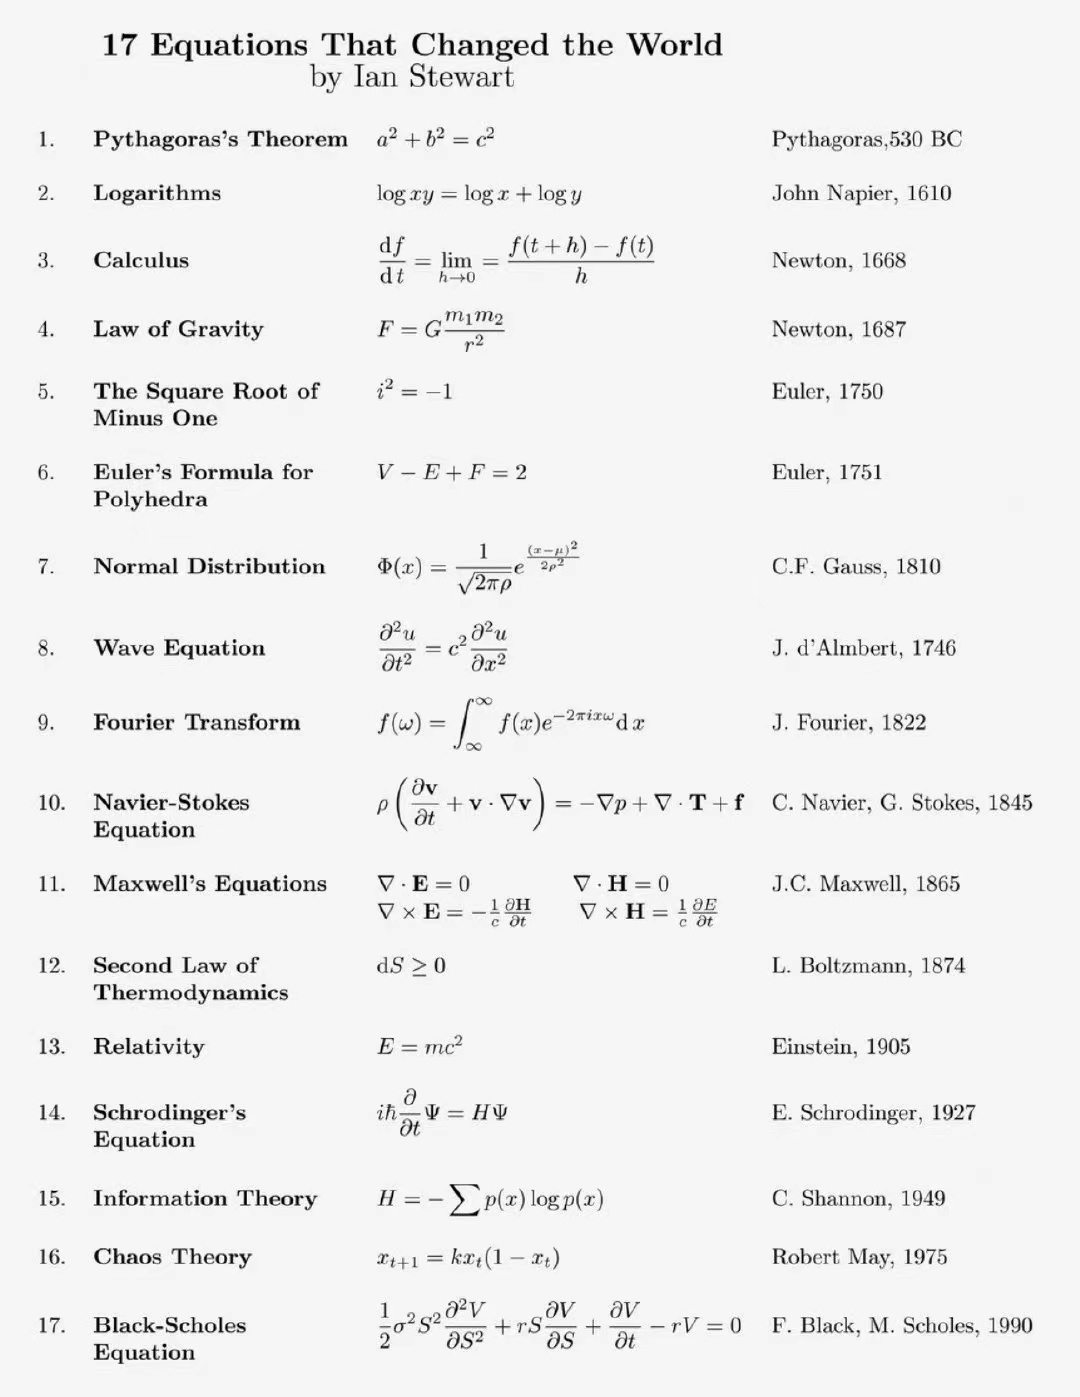
\includegraphics[height=2.85in,width=2.00in,viewport=0 0 780 1100,clip]{Figures/Great_Equation.jpg}
\label{Great_Equation}
\end{figure}
\end{minipage}
}

\frame
{
	\frametitle{量子力学的奠基人}
\begin{figure}[h!]
\centering
%\vspace{-25.5pt}
%\hspace*{-15.5pt}
%\includegraphics[height=0.57\textwidth,width=1.1\textwidth,viewport=0 0 2150 1050,clip]{Figures/Solvay_Conference-5-fine.jpg}
\vspace{-14.5pt}
\hspace*{-15.5pt}
\includegraphics[height=0.50\textwidth,width=0.70\textwidth,viewport=150 105 850 710,clip]{Figures/Solvay_Conference-5.jpg}
\caption{\fontsize{7.5pt}{6.2pt}\selectfont{\textrm{The Fifth Solvay International Conference, Brussels, Belgium, Oct. 1927}}}
\label{Solvay Conference-5-fine}
\end{figure}
\vspace{-11.5pt}
\fontsize{4.1pt}{3.9pt}\selectfont{\textrm{\textcolor{blue}{前排左起}:~I.Langmuir(\textcolor{blue}{朗缪尔}) M.Planck(\textcolor{blue}{普朗克}) Marie Curie(\textcolor{blue}{居里夫人}) H.Lorentz(\textcolor{blue}{洛仑兹}) A.Einstein(\textcolor{blue}{爱因斯坦}) P.Langevin(\textcolor{blue}{朗之万}) Ch.E.Guye(\textcolor{blue}{古伊}) C.T.R.Wilson(\textcolor{blue}{威尔逊}) O.W.Richardson(\textcolor{blue}{理查森})\\
\textcolor{blue}{中排左起}:~P.Debye(\textcolor{blue}{德拜}) M.Knudsen(\textcolor{blue}{克努森}) W.L.Bragg(\textcolor{blue}{布拉格}) H.A.Kramers(\textcolor{blue}{克莱默}) P.A.M.Dirac(\textcolor{blue}{狄拉克}) A.H.Compton(\textcolor{blue}{康普顿}) L.de Broglie(\textcolor{blue}{德布罗意}) M.Born(\textcolor{blue}{玻恩}) N.Bohr(\textcolor{blue}{玻尔})\\
\textcolor{blue}{后排左起}:~A.Piccard(\textcolor{blue}{皮卡尔德}) E.Henriot(\textcolor{blue}{亨利厄特}) P.Ehrenfest(\textcolor{blue}{埃伦费斯特}) Ed.Herzen(\textcolor{blue}{赫尔岑}) Th.de Donder(\textcolor{blue}{德唐德}) E.Schr\"odinger(\textcolor{blue}{薛定谔}) E.Verschaffelt(\textcolor{blue}{费尔夏费尔特}) W.Pauli(\textcolor{blue}{泡利}) W.Heisenberg(\textcolor{blue}{海森堡}) R.H.Fowler(\textcolor{blue}{富勒}) L.Brillouin(\textcolor{blue}{布里渊})}}
}

\frame
{
	\frametitle{态叠加原理:~\textrm{Schr\"odinger's cat}}
\begin{figure}[h!]
\centering
\vspace{-10.5pt}
\includegraphics[height=0.70\textwidth,width=0.48\textwidth,viewport=0 0 550 750,clip]{Figures/Schrodinger-cat.jpg}
\includegraphics[height=0.70\textwidth,width=0.50\textwidth,viewport=0 0 720 930,clip]{Figures/Schrodinger_book.jpg}
%\caption{\textrm{ABINIT}的Si.in}
\label{Schrodinger-cat}
\end{figure}
}

%\frame
%{
%	\frametitle{因果倒置:~\textrm{Delayed Choice Experiment}}
%\begin{figure}[h!]
%\centering
%\vspace{-10.5pt}
%\includegraphics[height=0.55\textwidth,width=1.0\textwidth,viewport=0 0 690 370,clip]{Figures/Schematic-diagram-of-delayed_choice-experiment.png}
%\caption{\fontsize{5.2pt}{3.9pt}\selectfont{\textrm{Schematic diagram of Wheeler's delayed choice experiment with A Mach-Zehnder Interferometer.}}}
%\label{Delayed_Choice-Experiment}
%\end{figure}
%}
%
\frame
{
	\frametitle{量子力学量力学}
\begin{figure}[h!]
\centering
\vspace{-13.5pt}
\includegraphics[height=0.75\textwidth,width=0.55\textwidth,viewport=0 0 500 650,clip]{Figures/Quote-Niels_Bohr-on-Quantum_mechanics.png}
\caption{\fontsize{5.2pt}{3.9pt}\selectfont{\textrm{A quote of Niels Bohr on Quantum mechanics.}}}
\label{Quote-Niels_Bohr}
\end{figure}
}

\frame
{
	\frametitle{几何原本:~公理体系的源头}
\begin{figure}[h!]
\centering
\vspace{-13pt}
\includegraphics[height=0.38\textwidth,width=0.65\textwidth,viewport=0 0 680 500,clip]{Figures/Element_Geometry_1.jpg}\\
\vspace{1pt}
\includegraphics[height=0.36\textwidth,width=0.65\textwidth,viewport=0 0 810 500,clip]{Figures/Element_Geometry_2.jpg}
%\caption{\textrm{ABINIT}的Si.in}
\label{Element_Geometru}
\end{figure}
}

\frame
{
	\frametitle{\textcolor{red}{公理体系}:~现代科学的逻辑起点}
\begin{figure}[h!]
\centering
\vspace{-10.5pt}
\includegraphics[height=0.68\textwidth,width=1.0\textwidth,viewport=0 0 770 500,clip]{Figures/Philp_Nature_Mach-2.png}
%\caption{\textrm{ABINIT}的Si.in}
\label{Philp_Nature}
\end{figure}
}

\frame[allowframebreaks]
{
	\frametitle{量子力学基本假设(\textcolor{red}{公理体系})}
	\begin{itemize}
		\item 全同粒子假设\\
			\textcolor{blue}{全同粒子组成的体系中,两个全同粒子相互调换不改变体系的状态}\\ 
			全同粒子是指\textcolor{red}{内禀性质完全相同的一类微观粒子}:\\例如,所有的电子是全同粒子 
		\item 波函数假设\\
			\textcolor{blue}{微观体系的运动状态可由波函数$\Psi$完全描述,波函数包含体系的所有性质}\\
			波函数$\Psi$一般要求满足\textcolor{red}{连续}、\textcolor{red}{有限}和\textcolor{red}{单值}三个条件
		\item 微观体系的运动状态\textcolor{blue}{波函数随时间变化的规律}:\\\textcolor{red}{遵从\textrm{Schr\"odinger}方程}
			$$\mathrm{i}\hbar\dfrac{\mathrm{d}}{\mathrm{d}t}|\Psi\rangle=\hat{\mathbf H}|\Psi\rangle$$
		\item 态叠加原理\\
			如果$\Psi_1$是体系的一个本征态,对应的本征值为$A_1$,$\Psi_2$也是体系的一个本征态,对应的本征值为$A_2$,则\textcolor{blue}{$$\Psi=C_1\Psi_1+C_2\Psi_2$$}\textcolor{red}{也是体系一个可能的存在状态}
		\item 力学量算符假设\\
			\textcolor{blue}{经典力学的物理量对应到量子力学中,要用线性~\textrm{Hermite}算符表示}(\textcolor{red}{\textrm{Hermite~}算符的本征函数构成完备空间})\\
			如动量算符 ~~~ $\hat{\mathbf{p}}=-\mathrm{i}\hbar\nabla$\\
			~~~位置算符 ~~~ $\hat{\mathbf r}=r$\\
			力学量算符之间有确定的对易关系(\textcolor{brown}{量子条件})
			$$[\hat{\mathbf F},\hat{\mathbf G}]=\hat{\mathbf F}\hat{\mathbf G}-\hat{\mathbf G}\hat{\mathbf F}$$ 
			
	\end{itemize}
}

\frame
{
	\frametitle{叠加态的数学表示:~矩阵}
\begin{figure}[h!]
\centering
\vspace{-1.5pt}
\hspace*{-0.12in}
\includegraphics[height=0.48\textwidth,width=1.05\textwidth]{Figures/Matrix_Rotation.png}
%\caption{\textrm{ABINIT}的Si.in}
\label{Matrix-Rotation}
\end{figure}
}

\frame
{
	\frametitle{量子化学学科创立}
	\begin{itemize}
		\item \textrm{1927}年,\textrm{\o.~Burrau}应用量子力学原理,完成\textrm{\ch{H2+}}离子的计算
		\item 同年,\textrm{Walter~Heitlery}和\textrm{Fritz~W.~London}对\textrm{\ch{H2}}分子的计算,标志着量子化学这一学科正式创立
	\end{itemize}
\begin{figure}[h!]
\centering
\vspace{-1.5pt}
\hspace*{-0.12in}
\includegraphics[height=0.48\textwidth,width=0.80\textwidth,viewport=0 10 260 175,clip]{Figures/Walter-Heitlery_Fritz-W-London.jpeg}
\caption{\textrm{W.~Heitlery (left) and F.~W.~London(right).}}
\label{Heitlery_London}
\end{figure}
}

%\frame
%{
%	\frametitle{\textrm{Paul Adrian Maurice Dirac's Commandments}}
%	\textrm{The underlying laws necessary for the mathematical treatment of a large part of physics \textcolor{red}{and the whole of chemistry} are thus completely known, and the difficulty lies only in the fact that application of these laws leads to equations that are \underline{too complex to be solved}.
%\vskip 15pt
%It therefore becomes desirable that approximation practical methods of applying quantum mechanics should be develop $\cdots$ 
%}

%\vskip 15pt
%\textrm{P.A.M Dirac Proc. Roy. Soc. Ser. A, \textbf{123}, 714, (1929)}
%}
%
\frame
{
%	\frametitle{\rm{Paul Dirac's Commandments\upcite{PRSLSA123-714_1929}}}
	\frametitle{\textrm{Paul Dirac's Commandments}}%\upcite{PRSLSA123-714_1929}}}
%	\textrm{\textcolor{purple}{The underlying laws necessary for the mathematical treatment of a large part of physics and the whole of chemistry are thus completely known, and the difficulty lies only in the fact that application of these laws leads to equations that are too complex to be solved.}}
\begin{figure}[h!]
\centering
\vspace{-10.5pt}
\includegraphics[height=0.71\textwidth,width=0.9\textwidth,viewport=0 0 1150 920,clip]{Figures/Dirac_comment.png}
%\caption{\textrm{ABINIT}的Si.in}
\label{Diract_Commandment}
\end{figure}
}

\section{自由电子气与密度泛函理论}       %Bookmark
\frame
{
	\frametitle{\textrm{Thomas-Fermi}模型} 
	\textrm{1927}年,\textrm{Thomas}和\textrm{Fermi}基于均匀电子气模型上建立\textrm{Thomas-Fermi}模型,\textcolor{blue}{体系能量可用}\textcolor{red}{电子密度}\textcolor{blue}{表示}:
	\begin{itemize}
		\item 动能表达式
			$$T_{\mathrm{TF}}[\rho(\vec r)]=\dfrac3{10}(3\pi^2)^{\frac23}\int\rho^{\frac53}(\vec r)\mathrm{d}\vec r$$
		\item 外势$V_{ext}(\vec r)$下电子体系的能量泛函表达式为
			\begin{displaymath}
				\begin{aligned}
					E_{\mathrm{TF}}[\rho(\vec r)]=&\dfrac3{10}(3\pi^2)^{\frac23}\int\rho^{\frac53}(\vec r)\mathrm{d}\vec r\\
					&+\int\rho(\vec r)V_{ext}(\vec r)\mathrm{d}\vec r+\dfrac12\int\int\dfrac{\rho(\vec r_1)\rho(\vec r_2)}{|\vec r_2-\vec r_1|}\mathrm{d}\vec r_1\mathrm{d}\vec r_2
				\end{aligned}
			\end{displaymath}
		\item \textrm{Thomas-Fermi}模型完全没有考虑电子的交换-相关作用
	\end{itemize}
}

\frame
{
	\frametitle{\textrm{Thomas-Fermi-Dirac}模型} 
	1930年,\textrm{Dirac}将\textrm{Thomas-Fermi}模型修正,用局域密度近似考虑电子交换作用
			\begin{displaymath}
				\begin{aligned}
					E_{\mathrm{TFD}}[\rho(\vec r)]=&\dfrac3{10}(3\pi^2)^{\frac23}\int\rho^{\frac53}(\vec r)\mathrm{d}\vec r+\int\rho(\vec r)V_{ext}(\vec r)\mathrm{d}\vec r\\
					&+\dfrac12\int\int\dfrac{\rho(\vec r_1)\rho(\vec r_2)}{|\vec r_2-\vec r_1|}\mathrm{d}\vec r_1\mathrm{d}\vec r_2-\dfrac34\bigg(\dfrac3{\pi}\bigg)^{\frac13}\int\rho^{\frac43}(\vec r)\mathrm{d}\vec r
				\end{aligned}
			\end{displaymath}
			\begin{itemize}
				\item 在总电子数守恒约束条件
					$$\int\rho(\vec r)\mathrm{d}\vec r=N$$
					下,能量泛函$E_{\mathrm{TFD}}[\rho(\vec r)]$对密度$\rho(\vec r)$的变分极小获得体系的基态密度和基态能量
			\end{itemize}
}

\frame
{
	\frametitle{\textrm{Thomas-Fermi}模型}
	\begin{itemize}
		\item \textrm{Thomas-Fermi}模型用电子密度代替波函数描述问题是极大的简化,但模型过于粗糙:\\
%			\begin{enumerate}
%				\item 以均匀电子气的密度得到动能的表达式
%				\item 完全忽略电子间的交换-相关作用
%			\end{enumerate}
			不能正确描述相互作用电子体系的基本特征,如原子的壳层结构
		\item \textrm{Thomas-Fermi}模型虽不够精确,但可以通过引入修正项校正:
			\textrm{Dirac}交换泛函 $$E_X[\rho(\vec r)]=-\dfrac34\bigg(\dfrac3{\pi}\bigg)^{\frac13}\int\rho^{\frac43}(\vec r)\mathrm{d}\vec r$$
			\textrm{Wigner}相关泛函 $$E_C[\rho(\vec r)]=-0.056\int\dfrac{\rho^{\frac43}(\vec r)}{0.079+\rho^{\frac13}(\vec r)}\mathrm{d}\vec r$$
	\end{itemize}
	\textrm{Thomas-Fermi}模型为密度泛函理论\textrm{(DFT)}提供了重要的启示
}

\frame                               %
{
\frametitle{密度泛函理论(\textrm{DFT})} %Slide Page Title
%   \secname
与传统的量子力学方法不同,密度泛函理论的基本变量是体系的基态电子密度。%通过体系的电子密度而非波函数确定体系的基态能量。
\begin{itemize}%[+-| alert@+>]
	\item 密度泛函理论的基石:\textrm{Hohenberg-Kohn}定理\upcite{PR136-B864_1964}
\vskip 5pt
\begin{itemize}%[+-| alert@+>]
   \setlength{\itemsep}{8pt}
 \item $E[\rho]=F_{\mathrm{HK}}[\rho]+\displaystyle\int\rho(\vec{r})v(\vec{r})\textrm{d}\vec{r}$ \\
\vskip 5pt 
{\fontsize{7.2pt}{6.2pt}\selectfont{其中$F_{\mathrm{HK}}[\rho]=\underset{\Psi\to\rho}{\mathrm{Min}}\langle\Psi[\rho]|\hat{T}+\hat{W}|\Psi[\rho]\rangle$
是普适的泛函表达式。}}\\%,指明多电子体系的基态性质与基态密度间存在一一对应关系
\textcolor{magenta}{\fontsize{8.2pt}{6.2pt}\selectfont{第一定理表明多电子体系的性质完全由体系的基态密度决定}}
   \item 如果$\tilde\Psi\neq\Psi$,
     $E[\tilde\rho]\geqslant E[\rho_0]$\\
     \textcolor{magenta}{\fontsize{8.2pt}{6.2pt}\selectfont{第二定理指出基态总能量泛函在体系基态电子密度处取极小值}}
   \end{itemize}
\vskip 8pt
 \item 密度泛函理论的优越性:~用密度($\rho$)代替波函数($\Psi$)描述体系
\vskip 5pt
 \item 密度泛函理论的困难:~能量密度泛函的精确形式未知
   \end{itemize}
}

\frame                               %
{
\frametitle{密度泛函理论(\textrm{DFT})}
\textrm{Kohn-Sham}方程\upcite{PR140-A1133_1965}:无相互作用体系+交换-相关能的贡献
$$(T_S+V_{e\!f\!f})|\varphi_i\rangle=\varepsilon_i|\varphi_i\rangle,\quad i=1,\cdots,N,\cdots$$
其中$T_S=-\dfrac12\nabla^2$~~是无相互作用体系的动能
\begin{displaymath}
	\begin{aligned}
		V_{e\!f\!f}(\vec r)=&V_{ext}(\vec r)+\displaystyle\int w(\vec r,\vec r\,')\rho(\vec r\,')\mathrm{d}\vec r\,'+V_{\mathrm{XC}}[\rho]\\
=&\displaystyle\int\dfrac{\rho(\vec r\,')}{|\vec r-\vec r^{\prime}|}\mathrm{d}\vec r\,'+V_{ext}(\vec r)+V_{\mathrm{XC}}[\rho]
	\end{aligned}
\end{displaymath}
$V_{ext}(\vec r)$是电子体系与外部的电荷或磁场相互作用\\
$V_{\mathrm{XC}}[\rho]=\dfrac{\delta E_{\mathrm{XC}}}{\delta\rho(\vec r)}$称为交换-相关势
\vskip 10pt
\textrm{Kohn-Sham}方程是形式上的单粒子方程
\vskip 6pt
\textrm{Kohn-Sham}方程的实质:\\\textcolor{red}{将动能泛函的主要部分分离出来,剩余部分放在交换-相关能中}
}

\frame
{
\frametitle{交换-相关能与交换-相关势}
实际考虑交换-相关能时,会将交换-相关能表示为交换能和相关能之和:
\begin{displaymath}
	E_{\mathrm{XC}}[\rho]=E_{\mathrm{X}}[\rho]+E_{\mathrm{C}}[\rho]=\int\varepsilon_{\mathrm{X}}[\rho]\rho(\vec{r}) \textrm{d}^3\vec{r}+\int\varepsilon_{\mathrm{C}}[\rho]\rho(\vec{r}) \textrm{d}^3\vec{r}
\end{displaymath}
$\varepsilon_{\mathrm{X}}[\rho]$和$\varepsilon_{\mathrm{C}}[\rho]$可理解为单电子的交换能和相关能
\vskip 20pt
交换-相关势通过交换-相关能计算得到:~
		\begin{displaymath}
			V_{\mathrm{XC}}^{\sigma}[\rho_{\alpha},\rho_{\beta}]=\dfrac{\delta E_{\mathrm{XC}}[\rho_{\alpha},\rho_{\beta}]}{\delta\rho_{\sigma}}=\dfrac{\delta\{E_{\mathrm{X}}[\rho_{\alpha},\rho_{\beta}]+E_{\mathrm{C}}[\rho_{\alpha},\rho_{\beta}]\}}{\delta\rho_{\sigma}}
		\end{displaymath}
		\textcolor{red}{注意}:~由于$E_{\mathrm{XC}}[\rho_{\sigma}]$对$\rho_{\sigma}$是非线性的
		\vskip 8pt
		\textcolor{blue}{$V_{\mathrm{XC}}=V_{\mathrm{X}}+V_{\mathrm{C}}$和$\varepsilon_{\mathrm{XC}}=\varepsilon_{\mathrm{X}}+\varepsilon_{\mathrm{C}}$不同},\underline{\textcolor{purple}{不要混淆这两个量}}
}
%  \beamertemplateshadingbackground{blue!10}{yellow!10}

\frame                               %
{
\frametitle{交换-相关能密度泛函}
\textcolor{blue}{密度泛函理论的核心问题}:\\
\textrm{Kohn-Sham}方程用于实际计算,必须知道$E_{XC}[\rho]$或者$V_{XC}[\rho]$与$\rho(\vec r)$的泛函关系
\vskip 5pt
\begin{minipage}[b]{0.59\textwidth}
 \hspace*{-20pt}
 \vskip -55pt
 \fontsize{7.5pt}{6.0pt}\selectfont{
 \begin{itemize}%[+-| alert@+>]
	 \setlength{\itemsep}{10pt}
 \item \textrm{LDA}:泛函只与密度分布的局域值有关
 \item \textrm{GGA}:泛函依赖:局域密度及其梯度
 \item $meta$-\textrm{GGA}:泛函依赖的变量还有动能密度
 \item 杂化(\textrm{hybrid})泛函:泛函与占据轨道有关
 \item 其他的交换-相关能泛函
 \item<1-> 完全非局域泛函:理想泛函,不现实
 \end{itemize}
}
\end{minipage}
\hfill
\begin{minipage}[b]{0.39\textwidth}
\begin{figure}[h!]
\centering
\hspace*{-15pt}
\includegraphics[height=1.7in,width=3.18in,viewport=10 5 1380 700,clip]{Figures/Jacobi-ladder.png}\\
%\caption{\tiny \textrm{}}%(与文献\cite{EPJB33-47_2003}图1对比)
\label{Jacob's_ladder}
\end{figure}
\vskip -10pt
\centering{\textcolor{red}{\textrm{\tiny Jacob's ladder}}}
\end{minipage}
% \begin{itemize}%[+-| alert@+>]
%\item 交换-相关能密度泛函
}

\frame                               %
{
	\frametitle{近似能量泛函$E_{\mathrm{XC}}[\rho]$的主要问题}
\vskip 20pt
\begin{enumerate}%[+-| alert@+>]
   \setlength{\itemsep}{10pt}
 \item  密度是整体变量:~电子自相互作用抵消不净\\%\quad\textrm{(LDA+U)}方法的校正%(\textrm{LDA+U})
	 用\textrm{DFT}计算电子数很少的体系,一般都会有较大的误差
 \item  电子相关:~简并和近简并基态的表示不合理\\
	 基态电子密度用不同的简并轨道计算时,体系能量应保持不变,但现有的近似能量泛函不具有这个性质
 \item  渐近行为:~处理弱相互作用体系的误差大\\
	 如\textrm{Van der Waals}相互作用和现有近似能量泛函本身的计算误差在同一量级
 \end{enumerate}
}

\frame                               %
{
	\frametitle{\textrm{Kohn-Sham}方程}
\begin{figure}[h!]
\centering
\vspace*{-0.21in}
\hspace*{-0.1in}
\includegraphics[height=2.7in,width=4.0in,viewport=2 5 1162 880,clip]{Figures/DFT.png}
\caption{\tiny \textrm{The Analysis of Kohn-Sham equation.}}%(与文献\cite{EPJB33-47_2003}图1对比)
\label{DFT}
\end{figure}
}

\frame
{
	\frametitle{\textrm{DFT-SCF}}
\begin{figure}[h!]
\centering
\vspace*{-0.25in}
\hspace*{-0.80in}
\includegraphics[height=2.80in,width=4.95in,viewport=5 3 1490 870,clip]{Figures/DFT-SCF_2.png}
%\caption{\tiny \textrm{Pseudopotential for metallic sodium, based on the empty core model and screened by the Thomas-Fermi dielectric function.}}%(与文献\cite{EPJB33-47_2003}图1对比)
\label{DFT-SCF-2}
\end{figure}
}

%\section{Induction on DFT and solid-state physics}       %Bookmark
\section{固体能带与赝势}       %Bookmark
\frame
{
%\frametitle{The Bloch theorem}
\frametitle{固体能带理论}
\begin{itemize}%[+-| alert@+>]
   \setlength{\itemsep}{8pt}
   \item 固体能带理论\upcite{Huang_Han}是固体电子理论的基础,形式上是\\单电子理论:
    $$\hat H |\psi_i^{\vec k}(\vec r)\rangle=\bigg[-\dfrac{\hbar^2}{2m}\nabla^2+V(\vec r)\bigg]|\psi_i^{\vec k}(\vec r)\rangle=\epsilon_i(\vec k)|\psi_i^{\vec k}(\vec r)\rangle$$
  \item \textrm{Bloch}定理:
%   \item \textrm{periodic potential:} $$V(\vec r)=V(\vec r+\vec R_n)$$
%     \textrm{Here,} $\vec R_n=n\vec R$
%   \item \textrm{Bloch theorem:}$$\psi_{\vec k}(\vec r)=\textrm{e}^{\textrm i\vec k\cdot\vec r}u_{\vec k}(\vec r)$$
%     \textrm{Here, $u_{\vec k}(\vec r)$ is a periodic function with the same periodicity as $V(\vec r)$, i.e., $u_{\vec k}(\vec r)=u_{\vec k}(\vec r+\vec R_n)$, then Bloch theorem could reads as:}
%     $$\psi_{\vec k}(\vec r+\vec R_n)=\textrm{e}^{\textrm i\vec k\cdot\vec R_n}\psi_{\vec k}(\vec r)$$
具有平移周期性的理想晶体,势能$V(\vec r)$满足$$V(\vec r)=V(\vec r+\vec R_n)$$
体系的波函数满足\textrm{Bloch}波函数形式:$$\psi_{\vec k}(\vec r)=\textrm{e}^{i\vec k\cdot\vec r}u_{\vec k}(\vec r)$$
是平面波和周期函数的乘积。$u(\vec r)$与势能有相同的周期。即$$u_{\vec k}(\vec r)=u_{\vec k}(\vec r+\vec R_n)$$
  \item 能带理论相当于分子轨道理论
%   \setlength{\itemsep}{30pt}
\item \textrm{Bloch}函数反映了波函数在周期性势场下的变化规律。
\end{itemize}
}

\frame
{
\frametitle{固体能带理论}
简并态微扰理论引起的能带裂分
\begin{figure}[h!]
\centering
%\hspace*{-10pt}
%\vspace*{-1.1in}
\includegraphics[height=2.1in,width=3.8in,viewport=10 90 570 380,clip]{Figures/Band_Gap.pdf}
\caption{\tiny \textrm{The Band-structure from free-electron gas.}}%
\label{Band-Structure-1}
\end{figure} 
}

\frame
{
\frametitle{固体能带理论}
从分子轨道到能带
\begin{figure}[h!]
\centering
\hspace*{-0.29in}
\vspace*{-0.1in}
\subfigure[一维$\mathrm{H}$原子链]{
\label{fig:Hydrogen-1D}
\includegraphics[height=0.25in,width=1.1in,viewport=70 255 570 375,clip]{Figures/Hydrogen-1D.pdf}}
\subfigure[$\mathrm{H}_n$分子轨道]{
\label{fig:Hydrogen-2-n}
\includegraphics[height=0.8in,width=1.5in,viewport=30 140 545 480,clip]{Figures/Hydrogen-Mol-Orbital.pdf}}
\subfigure[分子波函数]{
\label{fig:Hydrogen-Psi}
\vspace*{-0.2in}
\includegraphics[height=0.5in,width=1.4in,viewport=25 218 595 440,clip]{Figures/Hydrogen-Psi.pdf}}\\
\subfigure[分子轨道与能带]{
\label{fig:Hydrogen-Band-1D}
\includegraphics[height=0.6in,width=1.4in,viewport=35 215 575 450,clip]{Figures/Hydrogen-Band-1D.pdf}}
\subfigure[$d$\,轨道]{
\label{fig:Hydrogen-d-Band-1D}
\includegraphics[height=1.0in,width=0.7in,viewport=40 45 330 535,clip]{Figures/Hydrogen-d-Band-1D.pdf}}
\caption{\tiny \textrm{The Band-structure from Molecular-orbital.}}%
\label{Band-Structure-1}
\end{figure} 
}

\frame
{
\frametitle{周期体系的波函数}
物质的电子体系,可分为芯层分子和价层电子。芯电子能量低,受周围化学环境影响很小,基本保持原子属性;价层电子相互作用较强,对化学环境较为敏感。一般地,价电子波函数在原子间区域(\textrm{Interstitial}区)的变化平缓,在临近原子核附近区域(\textrm{Muffin-tin}球内),会出现剧烈振荡(与芯层波函数正交)。
\begin{figure}[h!]
\centering
\includegraphics[height=0.8in,width=4.in,viewport=41 433 539 546,clip]{Figures/Pseudo_wave.pdf}\\
\includegraphics[height=0.8in,width=4.in,viewport=41 210 539 339,clip]{Figures/Pseudo_wave.pdf}
\caption{\tiny \textrm{The periodic Potential and the wave functions in crystal.}}%(与文献\cite{EPJB33-47_2003}图1对比)
\label{Potential-Wave}
\end{figure}
}

\frame
{
%\frametitle{The methods on band structure calculation}
\frametitle{固体能带计算方法}
%\vskip 10pt
%\textrm{The mainly difference of all these methods below: the basis sets and the construction of the potential}
\vskip 10pt
常用的计算方法
\begin{itemize}%[+-| alert@+>]
%\begin{enumerate}%[+-| alert@+>]
\setlength{\itemsep}{15pt}
%  \item \textrm{Plane wave and the pseudo-potential}
	\item	平面波方法
	\item	正交平面波\textrm{(The orthogonalized plane wave, OPW)}和赝势\textrm{(Pseudo-potential, PP)}方法\upcite{Singh_Book,PRB41-7892_1990,JPCM6-8245_1994}
	\item	缀加平面波\textrm{(Augmented plane wave, APW)}方法
	\item	\textrm{MT}轨道\textrm{(Muffin-tin orbitals, MTO)}方法
	\item	投影子缀加波\textrm{(Projector Augmented Wave, PAW)}方法\upcite{PRB50-17953_1994,PRB59-1758_1999}
\end{itemize}
  \vskip 5pt 各种方法的主要区别:所选的基函数类型不同
}

%\frame
%{
%\frametitle{}
%\begin{figure}[h!]
%\centering
%\vspace*{-10pt}
%\includegraphics[height=2.80in,width=1.70in,viewport=60 90 325 500,clip]{WIEN2k_Program_flow.eps}
%\caption{\tiny \textrm{Program flow in \textbf{WIEN2k}.}}%(与文献\cite{EPJB33-47_2003}图1对比)
%\label{WIEN2k_program_flow}
%\end{figure}
%}

\frame
{
%\frametitle{The methods on band structure calculation}
	\frametitle{由\textrm{OPW}到赝势}
%\vskip 10pt
%\textrm{The mainly difference of all these methods below: the basis sets and the construction of the potential}
\begin{itemize}
\setlength{\itemsep}{5pt}
	\item 完全平面波基组,只要少数的平面波基组就可以很好地描述波函数在原子间的行为,近核的电子波函数则需要大量平面\\波展开。%因此完全平面波基组虽然方便,但求体系本征态对角化的矩阵非常巨大,计算变得异常耗时。
	\item 正交平面波(\textrm{Orthogonalized plane wave, OPW})方法,价电子用与芯层波函数正交的平面波展开,可以减少平面波数目
		\begin{displaymath}
			\phi_{OPW}^{\vec k+\vec G}(\vec r)=\phi_{PW}^{\vec k+\vec G}(\vec r)-\sum_{\alpha,c}\langle\varphi_c|\phi_{PW}^{\vec k+\vec G}\rangle\varphi_c(\vec r)
		\end{displaymath}
		并且势可以表示为$V^{eff}(\vec r)=V(\vec r)+V^R(\vec r)$,其中排斥部分是$$V^R(\vec r)=\sum_{\alpha,c}(\varepsilon_v-\varepsilon_c)|\varphi_c\rangle\langle\varphi_c|$$
\end{itemize}
}

\frame
{
\frametitle{赝势方法}
赝势(\textrm{Pseudo Potential, PP})方法是在正交平面波的基础上发展起来的,构造出平缓的势函数代替核的强吸引作用和芯层电子的排斥作用,用平缓的函数取代波函数近核时的震荡。
\begin{itemize}
\setlength{\itemsep}{5pt}
	\item 赝势-平面波方法,只需要少量平面波可展开赝波函数,大大提升了计算效率;但是赝波函数不能很好地反映与电子近核行为有关的性质。
	\item 赝势的构造并不唯一,考核构造赝势的两大指标:“柔软程度”\textrm{(Soft)}与“可移植性”\textrm{(transferability)}
\end{itemize}
\begin{figure}[h!]
\centering
\vspace*{-0.10in}
\includegraphics[height=1.35in,width=1.42in,viewport=154 100 562 508,clip]{Figures/Pseudo.pdf}
\includegraphics[height=1.35in,width=2.57in,viewport=1 1 980 500,clip]{Figures/Pseudo-2.png}
\caption{\tiny \textrm{The Pseudo wave function and Pseudo potential.}}%(与文献\cite{EPJB33-47_2003}图1对比)
\label{Pseudo_Potential-Wave}
\end{figure}
}

\frame
{
\frametitle{模守恒赝势和超软赝势}
\begin{itemize}
\setlength{\itemsep}{5pt}
	\item 模守恒\textrm{(Norm-conserving)}赝势,构造赝波函数有约束条件
		\begin{displaymath}
			\int_0^{r_c}\mathrm{d}\vec r\varphi^{\ast PS}(\vec r)\varphi^{PS}(\vec r)=\int_0^{r_c}\mathrm{d}\vec r\varphi^{\ast}(\vec r)\varphi(\vec r)
		\end{displaymath}
	模守恒赝势很好地解决了赝势的可移植性问题
	\item 超软\textrm{(Ultra-soft)}赝势,解除模守恒条件,实现对第一、第二周期元素的高效计算
\end{itemize}
\begin{figure}[h!]
\centering
\includegraphics[height=1.35in,width=1.40in,viewport=30 55 415 500,clip]{Figures/Norm-US-wave.pdf}
\caption{\tiny \textrm{Oxygen 2} \textit{p} \textrm{radical wave function (solid), NC-pseudo-wave (dottde) and US-pseudo-wave (dashed).}}%(与文献\cite{EPJB33-47_2003}图1对比)
\label{Norm-US-wave}
\end{figure}
}

\frame
{
\frametitle{超软赝势}
超软赝势在平缓的局域势函数$V^L(\vec r)$和赝波函数$|\phi_{lmj}(\vec r)\rangle$的基础上,构造函数
\begin{displaymath}
	|\chi_{lmj}(\vec r)\rangle=\bigg[\varepsilon_{lj}-\dfrac12\nabla^2-V^L(\vec r)\bigg]|\phi_{lmj}(\vec r)\rangle
\end{displaymath}
在此基础上得到矩阵$\mathbf{B}_{ij}=\langle\phi_i|\chi_j\rangle$和局域函数
\begin{displaymath}
	|\beta_i\rangle=\sum_j(\mathbf{B}^{-1})_{ji}|\chi_{j}\rangle
\end{displaymath}
因此非局域赝势可以表示为
\begin{displaymath}
	V_{NL}=\dfrac{|\chi_i\rangle\langle\chi_i|}{\langle\chi_i|\chi_i\rangle}=\sum_{i,j}\mathbf{B}_{ij}|\beta_i\rangle\langle\beta_j|
\end{displaymath}
用平缓函数构造赝波函数与真实波函数的电荷密度差
\begin{displaymath}
	Q_{nm}(\vec r)=\varphi_n^{\ast}(\vec r)\varphi_m(\vec r)-\tilde\varphi_n^{\ast}(\vec r)\tilde\varphi_m(\vec r)
\end{displaymath}
}

\frame
{
	\frametitle{}
\begin{figure}[h!]
\vspace*{-0.25in}
\centering
\includegraphics[height=2.80in,width=4.95in,viewport=5 3 1250 780,clip]{Figures/Method_Procedure.png}
%\caption{\tiny \textrm{Pseudopotential for metallic sodium, based on the empty core model and screened by the Thomas-Fermi dielectric function.}}%(与文献\cite{EPJB33-47_2003}图1对比)
\label{Method-Procedure}
\end{figure}
}

\section{\rm{FP-LAPW}方法}
\frame
{
\frametitle{\textrm{APW}方法和\textrm{LAPW}方法}
\begin{figure}[h!]
\centering
\includegraphics[height=1.10in,width=1.80in,viewport=40 150 545 465,clip]{Figures/Muffin_tin.pdf}
\includegraphics[height=1.10in,width=1.45in,viewport=1 20 485 435,clip]{Figures/APW.png}
\caption{\tiny \textrm{Partitioning of the unit cell into atomic spheres(I) and an interstitial region(II)}}%(与文献\cite{EPJB33-47_2003}图1对比)
\label{Muffin_tin}
\end{figure}
\begin{displaymath}
\hskip -28pt\footnotesize \varphi(\vec k_j,\vec r)=\left\{
  \begin{aligned}
    &\Omega^{-1/2}\exp[i\vec k_j\cdot\vec r],&|\vec r-\vec r_s|>R_{\mathrm{MT}}^s\\
    &\sum_{lm}A_{lm}u_l(|\vec r-\vec r_s|,E)Y_{lm}(\widehat{\vec r-\vec r_s}),&|\vec r-\vec r_s|\leqslant R_{\mathrm{MT}}^s
  \end{aligned}
\right.
\end{displaymath}
}

\frame
{
\frametitle{\textrm{APW}方法和\textrm{LAPW}方法}
%\small\textrm{APW}方法的困难,久期方程不能化成广义本征值方程的形式(久期方程对能量$E$是非线性的)为了克服这一困难,人们提出线性化方法,
\textrm{O.~K.~Andersen~}提出\textrm{LAPW}方法\upcite{Singh_Book}:将$u_l(r,E)$在某一合适的$E_l$值附近对$E$的一阶微商{\footnotesize$\left(\dfrac{\textrm{d}u_l(r,E)}{\textrm{d}E}\right)_{E_l}\equiv\dot u_l(r,E_l)$}\\代入\textrm{APW}基函数中可得\textrm{LAPW}方法的基函数:
$${\footnotesize\hskip -50pt \varphi(\vec k_j,\vec r)=\left\{
  \begin{aligned}
    &\Omega^{-1/2}\exp[i\vec k_j\cdot\vec r],&|\vec r-\vec r_s|>R_{\mathrm{MT}}^s\\
    &\sum_{lm}[A^{\vec k_j}_{lm}u_l(|\vec r-\vec r_s|,E_l)+B^{\vec k_j}_{lm}\dot u_l(|\vec r-\vec r_s|,E_l)]Y_{lm}(\widehat{\vec r-\vec r_s}),&|\vec r-\vec r_s|\leqslant R_{\mathrm{MT}}^s
  \end{aligned}
\right.}$$
%$$\Psi_{\vec k}(\vec r)=\int_{\Omega}\tilde G_{\vec k}(\vec r-\vec r\,^\prime;E)V(\vec r\,^\prime)\Psi_{\vec k}(\vec r\,^\prime)\textrm{d}\vec r\,^\prime$$
根据基函数在\textrm{MT}球面上连续到一阶,确定系数$A^{\vec k}_{lm}$,$B^{\vec k}_{lm}$的值。
\begin{figure}[h!]
\centering
\includegraphics[height=1.20in,width=1.98in,viewport=1 20 585 435,clip]{Figures/WIEN2k-LAPW.png}
\caption{\tiny \textrm{Partitioning of the unit cell into atomic spheres(I) and an interstitial region(II)}}%(与文献\cite{EPJB33-47_2003}图1对比)
\label{Muffin_tin}
\end{figure}
}
\frame
{
\frametitle{\textrm{LO}基函数}
为提高\textrm{LAPW}方法的变分自由度,在同一能量范围处理半芯态(接近价态的能量较高的芯态)和价态,可添加与$\vec k$无关的基函数,称为局域轨道(\textrm{local orbitals, LO})%。据此构造的基函数称为%包含两个指定能量的径向波函数和其中一个能量导数,这样的基函数即LAPW+
或\textrm{LO}基函数:
{\footnotesize
$$\hskip -40pt \phi_{lm}^{\mathrm{LO}}(\vec r)=\left\{
  \begin{aligned}
    &[A_{lm}u_l(r,E_{1,l})+B_{lm}\dot u_l(r,E_{1,l})+C_{lm}u_l(r,E_{2,l})]Y_{lm}(\hat{\vec r})\quad&r\leqslant R_{\mathrm{MT}}^s\\
    &0 &r>R_{\mathrm{MT}}^s
\end{aligned}
\right.$$}

类似地,根据$\phi_{lm}^{\mathrm{LO}}(\vec r)$在\textrm{MT}球面上的数值为零、一阶导数为零,并且$\phi_{lm}^{\mathrm{LO}}(\vec r)$在\textrm{MT}球内归一化的要求,可以确定系数$A_{lm}$,$B_{lm}$,$C_{lm}$的值。
\begin{figure}[h!]
	\vspace{-15pt}
\centering
\hspace{15pt}
\includegraphics[height=1.45in,width=1.55in,viewport=50 10 470 415,clip]{Figures/WIEN2k-lo.png}
\includegraphics[height=1.45in,width=1.45in,viewport=5 1 570 570,clip]{Figures/semi-core.png}
\caption{\tiny \textrm{}}%(与文献\cite{EPJB33-47_2003}图1对比)
\label{Muffin_tin_LO}
\end{figure}
}

\frame
{
\frametitle{\textrm{APW+lo}基函数}
\textrm{Sj\"ostedt}等发现上述\textrm{LAPW}方法并非是\textrm{APW}方法线性化的最有效方法。采用指定能量参数$E_l$的\textrm{APW}形式的径向波函数,外加\textrm{APW}型局域轨道(\textrm{local orbit, lo})基函数,是更有效的方案,称为\textrm{APW+lo}方法\upcite{SSC114-15_2000}。
$$  \varphi(\vec k_j,\vec r)=\left\{
  \begin{aligned}
    &\sum_{lm}[A^{\vec k_j}_{lm}u_l(r,E_l)]Y_{lm}(\hat{\vec r})\quad&r\leqslant R_{\mathrm{MT}}^s\\
    &\Omega^{-1/2}\exp(i\vec k_j\cdot\vec r) &r>R_{\mathrm{MT}}^s
  \end{aligned}\right.
  \label{eq:APW-basis}
$$
$$  \phi_{lm}^{\mathrm{lo}}(\vec r)=\left\{
  \begin{aligned}
  &[A_{lm}u_l(r,E_{1,l})+B_{lm}\dot u_l(r,E_{1,l})]Y_{lm}(\hat{\vec r})\quad&r\leqslant R_{\mathrm{MT}}^s\\
  &0&r>R_{\mathrm{MT}}^s
  \end{aligned}
\right.$$
\textrm{APW+lo}基函数式形式上与标准\textrm{LAPW}基函数式形式非常相似,但\textrm{APW+lo}基函数是平滑且一阶可微的,在\textrm{MT}球面上有动能对\textrm{Hamiltonian}的贡献需要计算。计算表明,采用\textrm{APW+lo}基组比标准\textrm{LAPW}基组计算效率高。
}

\frame
{
\frametitle{\textrm{WIEN2k}程序中基函数的选择}
\vskip 10pt
\begin{itemize}
\setlength{\itemsep}{15pt}
	\item 对$s$态、$p$态价电子轨道用\textrm{LAPW}基组展开
	\item 对一般平面波基函数展开收敛缓慢的轨道(如过渡金属的3$d$态波函数)或\textrm{MT}球半径特别小的体系用\textrm{APW+lo}基组展开
	\item 对半芯层轨道用\textrm{LAPW-LO}基组展开
\end{itemize}
这样搭配选择基组,可以同时较好地处理价态和半芯态。
}

\frame
{
\frametitle{\textrm{WIEN2k}程序中基函数的选择}
\begin{figure}[h!]
	\vspace{-15pt}
\centering
\hspace{15pt}
\includegraphics[height=2.55in,width=3.35in,viewport=10 30 750 605,clip]{Figures/WIEN2k-in1.png}
\caption{\tiny \textrm{The parameter $\mathrm{E}_l$ in case.in1 for WIEN2k.}}%(与文献\cite{EPJB33-47_2003}图1对比)
\label{WIEN2k-in1}
\end{figure}
}

\frame
{
\frametitle{全势的基本思想}
全势\textrm{(Full Potential, FP)}是相对于赝势的概念,即\textcolor{blue}{电子运动过程中感受到其它粒子作用的真实效果}。
实际计算中,构造\textrm{LAPW}基组的\textrm{MT}势换成晶体势函数。一般地,在每个\textrm{MT}球内,势函数用球谐函数(或者是满足晶体对称性)展开,\textrm{MT}球外的势函数用\textrm{Fourier}级数展开:%\upcite{PRB13-5362_1976}
{\footnotesize$$ V(\vec r)=\left\{
  \begin{aligned}
    &\sum_{a,L}V_L^a(r)Y_L(\hat{\vec r})\quad &r\leqslant R_{\mathrm{MT}}^a\\
    &\sum_{\vec G_n}V_I(\vec G_n)\textrm{e}^{i\vec G_n\cdot\vec r} &\vec r\in\mathrm{II}
  \end{aligned}\right.
  \label{eq:solid-63}
$$}
这里$L$\,$\equiv$\,$l,m$,$\vec G_n$为倒格矢,$Y_L(\hat{\vec r})$是球谐函数,\textrm{II}为原子间区域。
\begin{itemize}
	\item 在\textrm{MT}球内靠近原子核,势能具有原子型势能特征
	\item 在\textrm{MT}球外,要满足\textrm{Bloch}函数边界条件特征。
	\item 在\textrm{MT}球内外的势能表象不同,同样要求势能在\textrm{MT}球表面连续。
\end{itemize}
}

\frame
{
\frametitle{全势的基本思想}
\vspace*{-13pt}
\begin{figure}[h!]
\centering
\includegraphics[height=2.70in,width=2.02in,viewport=1 22 507 715,clip]{Figures/MT_FP.png}
\caption{\tiny \textrm{From Muffin-tin Potential to Full Potential}}%(与文献\cite{EPJB33-47_2003}图1对比)
\label{Muffin_tin_LO}
\end{figure}
}

\frame
{
\frametitle{全势的基本思想}
由此得到晶体的势函数为\upcite{Comp_Method}
$$ V(\vec r)=V_{MT}(\vec r)+V_{WMT}(\vec r)+V_{NS}(\vec r)
  \label{eq:solid-64}
$$
\begin{itemize}
	\item $V_{MT}(\vec r)$是简单的\textrm{MT}势(包括\textrm{MT}球内球对称部分和\textrm{MT}球外常数势)
	\item $V_{WMT}(\vec r)$表示\textrm{MT}球外势能\textrm{Fourier}展开对\textrm{MT}常数势的偏离,仅在\textrm{MT}球外非零,球内为零
	\item $V_{NS}(\vec r)$是势能在\textrm{MT}球内对球对称性的偏离,只在\textrm{MT}球内有非零值
\end{itemize}
\textbf{\large 为求得交换-相关势$V_{XC}$,将电荷密度也采用类似的形式展开。}
}
\frame
{
\frametitle{全势方法在$\vec k$空间中的实现}
\textrm{WIEN2k}程序包采用\textrm{Weiner}提出全势计算方法\upcite{JMP22-2433_1981}。
\begin{itemize}
	\item 将\textrm{MT}球外的电荷密度(常数)扩展到球内,并在正空间内作多极矩展开$Q_{PW}(\vec r)\quad(r\leqslant R_{\mathrm{MT}}^s)$
	\item 根据\textrm{MT}球内的电荷密度分布,电子密度在正空间分布的多极矩$Q_{MT}(\vec r)\quad(r\leqslant R_{\mathrm{MT}}^s)$
	\item 构造赝电荷密度$\tilde\rho(\vec r)$,要求$\tilde\rho(\vec r)$在空间分布平缓(方便\textrm{Flourier}变换),其多级矩$\tilde Q_{MT}(\vec r)\quad(r\leqslant R_{\mathrm{MT}}^s)$为真实电荷密度多极展开多极矩与延伸到球内的电荷多极矩之差\\
	\item 在$\vec k$空间内,体系\textrm{MT}球外真实电荷密度叠加\textrm{MT}球内赝电荷密度,根据\textrm{Coulomb}定理计算得到\textrm{Coulomb}势在间隙区的表达式$V_C(\vec k)$
	\item 以\textrm{MT}球面的势能为球形\textrm{Dirichlet}边值条件,计算\textrm{MT}球内电子的\textrm{Coulomb}势$V(\vec r)$
\end{itemize}
}
\frame
{
\frametitle{总能量的计算}
\textrm{WIEN2k}程序中,\textrm{WS}原胞内的总能量可以表示为\upcite{PRB26-4571_1982}:
{\footnotesize
\begin{displaymath}
\begin{split}
E_T=&\sum_i\varepsilon_i-\frac12\int_{\Omega}\rho(\vec r)[V_C(\vec r)+2\mu_{XC}(\vec r)]\mathrm{d}\vec r-\frac12\sum_{\nu}Z_{\nu}V_M(\vec r_{\nu})+E_{XC}[\rho] \\
   =&\sum_i\varepsilon_i-\frac12\left(\int_{\Omega}\rho(\vec r)V_C(\vec r)\mathrm{d}\vec r+\sum_{\nu}Z_{\nu}\bigg\langle\frac1r\rho(\vec r)\bigg\rangle_{\nu}\right)-%\dfrac12
   \int_{\Omega}\rho(\vec r)\mu_{XC}(\vec r)\mathrm{d}\vec r \\
   &-\frac12\sum_{\nu}\frac{Z_{\nu}}{R_{\nu}}[R_{\nu}S_0(R_{\nu})+Z_{\nu}-Q_{\nu}]+E_{XC}[\rho]
\end{split}
\end{displaymath}
}
这里$V_C(\vec r)\!=\!\displaystyle\int\dfrac{\rho(\vec r\,^\prime)}{|\vec r-{\vec r}\,^\prime|}\mathrm{d}\vec r\,^\prime-\sum\limits_{\alpha}\dfrac{Z_{\alpha}}{|\vec r-\vec r_{\alpha}|}$,$\mu_{XC}$为交换-相关势。
}
\frame
{
\frametitle{原子核位置能量奇点排除}
核吸引势和\textrm{Coulomb}势在原子核位置都存在奇点,单独求和,总能量是发散的。

为排除奇点,将\textrm{Coulomb}势能和电荷密度在各原子核附近用球谐函数展开,在原子核附近,有
{\footnotesize\begin{displaymath}
  \begin{split}
    &\int_{\Omega}\rho(\vec r)V_C(\vec r)\mathrm{d}\vec r+Z_{\nu}\sqrt{4\pi}\int_0^{R_{\nu}}\mathrm{d}rr^2\frac{\rho_{00}(r)}r\\
    =&\sqrt{4\pi}\int_{\Omega}\mathrm{d}rr^2\rho_{00}(\vec r)\left(\dfrac1{\sqrt{4\pi}}V_{00}(r)+\frac{Z_{\nu}}r\right)+\sum_{lm>0}\int\mathrm{d}rr^2\rho_{lm}(r)V_{lm}(r)
  \end{split}
\end{displaymath}}
\textrm{Coulomb}势的奇点只出现在$V_{00}(r)$中,将$V_{00}(r)$写成核的点电荷势与源于电子的平缓的势$\hat V_{00}(r)$两部分之和,
\footnotesize{$$V_{00}(r)=-\sqrt{4\pi}\frac{Z_{\nu}}r+\hat V_{00}(r)$$}
可以看出\textrm{Coulomb}势的奇点被消去了。\\有必要指出的是,这样方式可以将总能量中的奇点排除,但是单独每一项在原子核位置仍然是发散的。
}
\frame
{
	\frametitle{\textrm{LDA}近似下的总能量表达式}
\begin{itemize}
	\item 间隙区的电荷密度用平面波展开:\footnotesize{$\rho(\vec r)=\sum\limits_{\vec G}\rho(\vec G)\mathrm{e}^{i\vec G\cdot\vec r}$}
	\item 在\textrm{MT}球内,电荷密度用球谐函数展开,在动量空间中的展开形式为:\footnotesize{$\bar\rho_{lm}(r_{\nu})=4\pi i^l\sum\limits_{\vec G}\rho(\vec G)\mathrm{e}^{i\vec G\cdot\vec r_{\nu}}j_l(\vec G\cdot\vec r_{\nu})Y_{lm}^{\ast}(\vec G)$}
\end{itemize}
\textrm{LDA}近似下,\footnotesize{$$E_{XC}[\rho]\approx\int_{\Omega}\rho(\vec r)\varepsilon_{XC}(\vec r)\textrm{d}\vec r$$}
因此\textrm{WS}原胞内的晶体总能量可以写成:
{\footnotesize
\begin{displaymath}
  \begin{split}
\hskip -10pt	  E=&\sum_i\varepsilon_i-\Omega\sum_{\vec G}\rho(\vec G)\tilde V^{\ast}(\vec G)-\frac12\sum_{\nu}\dfrac{Z_{\nu}}{R_{\nu}}[Z_{\nu}-Q_{\nu}+R_{\nu}S_0(R_{\nu})]\\
    &-\sum_{\nu}\sum_{lm}\int_0^{R_{\nu}}\mathrm{d}rr^2\left[\rho_{lm}(r_{\nu})\left(\tilde V_{lm}^{\ast}(r_{\nu})+\dfrac{\sqrt{4\pi}}{2r_{\nu}}Z_{\nu}\delta_{l0}\right)-\bar\rho_{lm}(\vec r_{\nu})\bar V_{lm}^{\ast}(\vec r_{\nu})\right]
  \end{split}
  \label{eq:solid-83}
\end{displaymath}}
这里$\tilde V(\vec r)$和$\bar V_{lm}(\vec r)$根据都按下式计算:
\footnotesize{$$\tilde V(\vec r)=\frac12V_C(\vec r)-\varepsilon_{XC}(\vec r)+\mu_{XC}(\vec r)$$}
}

\frame
{
\frametitle{}
\begin{figure}[h!]
\centering
\hspace*{-10pt}
\includegraphics[height=1.72in,width=4.2in,viewport=30 165 550 375,clip]{Figures/WIEN2k_Data_flow.pdf}
\caption{\tiny \textrm{Data flow during a SCF cycle (programX.def, case.struct, case.inX, case.outputX and optional files are omitted).}}%(与文献\cite{EPJB33-47_2003}图1对比)
\label{WIEN2k_Data_flow}
\end{figure}
}
%\section{PAW方法的基本思想}
%\frame
%{
%\frametitle{PAW方法基本思想}
%\textrm{P. E. Bl\"ochl}尝试了结合赝势方法和\textrm{APW}方法优势的\textrm{(Projected Augmented Wave, PAW)}方法\upcite{PRB50-17953_1994,PRB59-1758_1999}。
%\begin{itemize}
%\setlength{\itemsep}{8pt}
%	\item 与芯层态正交的全部价电子构成的\textrm{Hilbert}空间,价电子彼此的正交使得波函数在\textrm{Muffin-tin}球内振荡
%	\item 作线性变换,将原\textrm{Hilbert}空间变换为赝\textrm{Hilbert}空间,相应的价电子波函数变换为赝波函数
%		$$|\Psi\rangle=\tau|\tilde\Psi\rangle$$
%	\item 赝波函数与全电子波函数在\textrm{Interstitial}区变换前后保持不变,在\textrm{Muffin-tin}球内的波函数变换后可使计算极大的方便\\
%		$$\langle A \rangle=\langle\Psi|\mathrm{A}|\Psi\rangle=\langle\tilde\Psi|\tau^{\dag}\mathrm{A}\tau|\tilde\Psi\rangle=\langle\tilde\Psi|\tilde{\mathrm{A}}|\tilde\Psi\rangle$$
%	$$\tau=1+\sum_{\mathrm R}\hat\tau_{\mathrm R}$$
%	这里每个$\hat\tau_{\mathrm R}$作用的区域是每个原子核附近的\textrm{Muffin-tin}区$\Omega_{\mathrm R}$
%\end{itemize}
%}

%\frame
%{
%\frametitle{PAW方法基本思想}
%$\hat\tau_{\mathrm R}$的定义是在\textrm{Muffin-tin}球区,$\hat\tau_{\mathrm R}$使得赝原子波函数$\tilde\phi_i$与全原子波函数$\phi_i$之间的变换关系满足:
%$$|\phi_i\rangle=(1+\hat\tau_{\mathrm R})|\tilde\phi_i\rangle$$

%在每个\textrm{Muffin-tin}球内,体系的赝波函数用赝原子波函数展开:
%$$|\tilde\Psi\rangle=\sum_i|\tilde\phi_i\rangle c_i$$
%由于$|\phi_i\rangle=\tau|\tilde\phi_i\rangle$,因此\textrm{Muffin-tin}球内全电子波函数可以表示为:
%$$|\Psi\rangle=\tau|\tilde\Psi\rangle=\sum_i|\phi_i\rangle c_i$$
%因此,全电子波函数可以表示为:
%$$|\Psi\rangle=|\tilde\Psi\rangle-\sum_i|\tilde\phi_i\rangle c_i+\sum_i|\phi_i\rangle c_i$$
%}

%\frame
%{
%\frametitle{投影函数及其特征}
%为了确保$\tau$是线性变换,它必须是赝波函数$\tilde\Psi$的线性函数。因此系数$c_i$满足:
%$$c_i=\langle\tilde p_i|\tilde\Psi\rangle$$
%这里$\tilde p_i$称为投影函数\textrm{(projector functions)}。
%投影函数要满足的条件:
%\begin{itemize}
%	\item $$\sum_i|\tilde\phi_i\rangle\langle\tilde p_i|=1$$
%	\item $$\langle\tilde p_i|\tilde\phi_j\rangle=\delta_{ij}$$
%\end{itemize}
%投影函数最一般的形式可以表示为:
%$$\langle\tilde p_i|=\sum_j(\{\langle f_k|\tilde\phi_l\rangle\})_{ij}^{-1}\langle f_j|$$
%这里$|f_j\rangle$组合成一套线性无关的函数。
%}

%\frame
%{
%\frametitle{}
%线性变换算符可以表示为:
%$$\tau=1+\sum_i(|\phi_i\rangle-|\tilde\phi_i\rangle)\langle\tilde p_i|$$
%因此,全电子波函数的表达式为:
%$$|\Psi\rangle=|\tilde\Psi\rangle+\sum_i(|\phi_i\rangle-|\tilde\phi_i\rangle)\langle\tilde p_i|\tilde\Psi\rangle$$

%对于芯层态$|\Psi^c\rangle$,处理与价层态类似:
%$$|\Psi^c\rangle=|\tilde\Psi^c\rangle+|\phi^c\rangle-|\tilde\phi^c\rangle$$
%但芯层态不需要定义相应的投影函数,本质上是冻芯近似的处理方式。
%}

%\frame
%{
%\frametitle{PAW方法的算符和密度表示}
%因为引入变换算符$\tau$,波函数由\textrm{Schr\"odinger}表象变为\textrm{Heisenberg}表象。因此在赝波函数构成的\textrm{Hilbert}空间内,算符的变换满足:
%\begin{displaymath}
%\begin{aligned}
%	\tilde A &=\tau^{\dag}A\tau \\
%			&=A+\sum_{i,j}|\tilde p_i\rangle(\langle\phi_i|A|\phi_j\rangle-\langle\tilde\phi_i|A|\tilde\phi_j\rangle)\langle\tilde p_j|
%\end{aligned}
%\end{displaymath}
%由此,可以得到电荷密度的表达式为:
%$$n(\vec r)=\tilde n(\vec r)+n^1(\vec r)-\tilde n^1(\vec r)$$
%\footnotesize{
%这里
%$$\tilde n(\vec r)=\sum_nf_n\langle\tilde\Psi_n|\vec r\rangle\langle\vec r|\tilde\Psi_n\rangle$$
%$$n^1(\vec r)=\sum_{n,(i,j)}f_n\langle\tilde\Psi_n|\tilde p_i\rangle\langle\phi_i|\vec r\rangle\langle\vec r|\phi_j\rangle\langle\tilde p_j|\tilde\Psi_n\rangle$$
%$$\tilde n^1(\vec r)=\sum_{n,(i,j)}f_n\langle\tilde\Psi_n|\tilde p_i\rangle\langle\tilde\phi_i|\vec r\rangle\langle\vec r|\tilde\phi_j\rangle\langle\tilde p_j|\tilde\Psi_n\rangle$$
%}}

%\frame
%{
%	\frametitle{总能量的表示}
%总能量泛函
%\begin{displaymath}
%	\begin{aligned}
%		E&=\sum_nf_n\langle\Psi_n|-\dfrac12\nabla^2|\Psi_n\rangle\\
%		 &+\dfrac12\int\mathrm{d}\vec r\int\mathrm{d}\vec r^{\prime}\dfrac{(n+n^Z)(n+n^Z)}{|\vec r-\vec r^{\prime}|}+\int\mathrm{d}\vec r n\epsilon_{\mathrm{XC}}(n)
%	\end{aligned}
%\end{displaymath}
%与密度表达式类似,$E=\tilde E+E^1-\tilde E^1$,每一项分别表示为:
%\footnotesize{
%\begin{displaymath}
%	\begin{aligned}
%		\tilde E&=\sum_nf_n\langle\tilde\Psi_n|-\dfrac12\nabla^2|\tilde\Psi_n\rangle\\
%		 &+\dfrac12\int\mathrm{d}\vec r\int\mathrm{d}\vec r^{\prime}\dfrac{(\tilde n+\hat n)(\tilde n+\hat n)}{|\vec r-\vec r^{\prime}|}+\int\mathrm{d}\vec r \tilde n\bar v+\int\mathrm{d}\vec r \tilde n\epsilon_{\mathrm{XC}}(\tilde n)
%	\end{aligned}
%\end{displaymath}
%\begin{displaymath}
%	\begin{aligned}
%		E^1&=\sum_{n,(i,j)}f_n\langle\tilde\Psi_n|\tilde p_i\rangle\langle\phi_i-\dfrac12\nabla^2|\phi_j\rangle\tilde p_j\tilde\Psi_n\rangle\\
%		 &+\dfrac12\int\mathrm{d}\vec r\int\mathrm{d}\vec r^{\prime}\dfrac{(n^1+n^Z)(n^1+n^Z)}{|\vec r-\vec r^{\prime}|}+\int\mathrm{d}\vec r n^1\epsilon_{\mathrm{XC}}(n^1)
%	\end{aligned}
%\end{displaymath}
%\begin{displaymath}
%	\begin{aligned}
%		\tilde E^1&=\sum_{n,(i,j)}f_n\langle\tilde\Psi_n|\tilde p_i\rangle\langle\tilde\phi_i-\dfrac12\nabla^2|\tilde\phi_j\rangle\tilde p_j\tilde\Psi_n\rangle\\
%		 &+\dfrac12\int\mathrm{d}\vec r\int\mathrm{d}\vec r^{\prime}\dfrac{(\tilde n^1+\hat n)(\tilde n^1+\hat n)}{|\vec r-\vec r^{\prime}|}+\int\mathrm{d}\vec r \tilde n^1\bar v+\int\mathrm{d}\vec r \hat n^1\epsilon_{\mathrm{XC}}(\hat n^1)
%	\end{aligned}
%\end{displaymath}
%}}

%\frame
%{
%	\frametitle{补偿电荷密度$\hat n$的计算}
%$n^Z$表示原子核位置的点电荷密度,$\hat n$称为补偿电荷密度。\\
%$\hat n$的作用:\large{\bf 使$(n^1+n^Z)$与$(\hat n^1+\hat n)$具有相同的多极矩展开},并且$\hat n=\sum\nolimits_R\hat n_R$,在每个\textrm{Muffin-tin}球内:
%$$\hat n_R(r)=\sum_Lg_{RL}(r)Q_{RL}$$
%其中
%$$g_{RL}(r)=C_l|\vec r-\vec R|^lY_L(r-R)\mathrm{e}^{-(|\vec r-\vec R|/r_c)^2}$$
%$$Q_{RL}=\int\mathrm{d}\vec r|\vec r-\vec R|^l[n^1_R(\vec r)+n^Z_R(\vec r)-\tilde n^1_R(\vec r)]Y^{\ast}_L(\vec r-\vec R)$$
%如果直接计算$\hat n_R(r)$,\textrm{Gaussian}函数非常尖锐。实际计算时引入赝补偿电荷$\hat n^{\prime}$,它与$\hat n$具有相同的多极矩展开,但相应的级数$g^{\prime}_{RL}(r)$平缓得多。
%}

%\frame
%{
%	\frametitle{}
%因此$\tilde E$中的静电相互作用的表达式为:
%\begin{displaymath}
%	\begin{aligned}
%		&\dfrac12\int\mathrm{d}\vec r\int\mathrm{d}\vec r^{\prime}\dfrac{(\tilde n+\hat n)(\tilde n+\hat n)}{|\vec r-\vec r^{\prime}|}\\
%	=&\dfrac12\int\mathrm{d}\vec r\int\mathrm{d}\vec r^{\prime}\dfrac{(\tilde n+\hat n^{\prime})(\tilde n+\hat n^{\prime})}{|\vec r-\vec r^{\prime}|}\\
%		&+\int\mathrm{d}\vec r\int\mathrm{d}\vec r^{\prime}\tilde n(\vec r)\dfrac{\hat n(\vec r^{\prime})-\hat n^{\prime}(\vec r^{\prime})}{|\vec r-\vec r^{\prime}|}\\
%		&+\sum_{\vec R,\vec R^{\prime}}\dfrac12\int\mathrm{d}\vec r\int\mathrm{d}\vec r^{\prime}\dfrac{\hat n_R(\vec r)\hat n_{R^{\prime}}(\vec r^{\prime})-\hat n^{\prime}_R(\vec r)\hat n^{\prime}_{R^{\prime}}(\vec r^{\prime})}{|\vec r-\vec r^{\prime}|}
%	\end{aligned}
%\end{displaymath}
%}

%\frame
%{
%	\frametitle{PAW方法的重叠算符和Hamilton算符}
%重叠算符:
%$$\tilde O=1+\sum_{i,j}|\tilde p_i\rangle[\langle\phi_i|\phi_j\rangle-\langle\tilde\phi_i|\tilde\phi_j\rangle]\langle\tilde p_j|$$
%\textrm{Hamiliton}算符
%\begin{itemize}
%	\item 动能算符:
%		$$\tilde T=-\dfrac12\nabla^2+\sum_{i,j}|\tilde p_i\rangle[\langle\phi_i|-\dfrac12\nabla^2|\phi_j\rangle-\langle\tilde\phi_i|-\dfrac12\nabla^2|\tilde\phi_j\rangle]\langle\tilde p_j|$$
%	\item 完全势\textrm{(full-potential)}算符:
%$$v(\vec r)=\tilde v(\vec r)+v^1(\vec r)-\tilde v^1(\vec r)$$
%	\item \textrm{Hamilton}算符:
%		$$\tilde H=-\dfrac12\nabla^2+\tilde v+\sum_{i,j}|\tilde p_i\rangle[\langle\phi_i|-\dfrac12\nabla^2+v^1|\phi_j\rangle-\langle\tilde\phi_i|-\dfrac12\nabla^2+\tilde v^1|\tilde\phi_j\rangle]\langle\tilde p_j|$$
%\end{itemize}
%}

%\frame
%{
%	\frametitle{分波函数$\phi_i$的构造}
%	\begin{itemize}
%		\item 全电子分波函数由方程:
%			$$\biggl(\dfrac12\nabla^2+v_{at}-\epsilon_i^1\biggr)|\phi_i\rangle=0$$
%			计算得到
%		\item 赝势分波函数由方程:
%			$$\biggl(\dfrac12\nabla^2+w_{i}(\vec r)-\epsilon_i^1\biggr)|\tilde\phi_i\rangle=0$$
%			计算得到。\\
%			这里$w_i(\vec r)=\tilde v_{at}(\vec r)+c_ik(\vec r)$,由赝势$\tilde v_{at}(\vec r)$确定。\\
%		\item 赝势$\tilde v_{at}(\vec r)$的确定:对不含\textit{d}电子体系与过渡元素体系采用不同的形式。
%		\end{itemize}
%}

%\frame
%{
%	\frametitle{投影函数$\tilde p_i$的构造}
%	\begin{itemize}
%		\item $\tilde p_i$由递推方式得到,初始的$\tilde p_i$的生成:
%			$$|\tilde p_i\rangle=\biggl(\dfrac12\nabla^2+\tilde v_{at}-\epsilon_i^1\biggr)|\tilde\phi_i\rangle$$
%		\item 根据正交关系$\langle\tilde p_i|\tilde\phi_j\rangle=\delta_{ij}$有:
%			$$|\tilde p_i\rangle=|\tilde p_i\rangle-\sum_{j=1}^{i-1}|\tilde p_j\rangle\langle\tilde\phi_j|\tilde p_i\rangle$$
%		为确保分波函数与投影函数正交:
%			$$|\phi_i\rangle=|\phi_i\rangle-\sum_{j=1}^{i-1}|\phi_j\rangle\langle\tilde p_j|\tilde\phi_i\rangle$$
%			$$|\tilde\phi_i\rangle=|\tilde\phi_i\rangle-\sum_{j=1}^{i-1}|\tilde\phi_j\rangle\langle p_j|\tilde\phi_i\rangle$$
%		\end{itemize}
%}
%\frame
%{
%\frametitle{}
%		最终的投影函数和分波函数的表达式为:
%			$$|\tilde p_i\rangle=|\tilde p_i\rangle/\langle\tilde p_i|\tilde\phi_i\rangle\times c$$
%			$$|\tilde\phi_i\rangle=|\tilde\phi_i\rangle/c$$
%			$$|\phi_i\rangle=|\phi_i\rangle/c$$
%			$c$是为防止数值误差引入的常数。
%}

%\frame
%{
%\frametitle{PAW方法和US-PP方法}
%\begin{itemize}
%\setlength{\itemsep}{15pt}
%	\item \textrm{PAW}方法在\textrm{Muffin-tin}球内使用的是原子真实势和全电子波函数
%	\item \textrm{PAW}方法提供了体系全电子波函数与赝波函数之间的变换关系
%	\item 赝势方法计算重叠矩阵和电荷密度依赖于所构造赝势的散射性质,\textrm{PAW}方法则利用赝电荷多极矩方式更合理地实现
%	\item 因为\textrm{PAW}方法使用原子径向函数,平面波截断大大降低,比传统的赝势方法计算效率更高
%	\end{itemize}
%}

%\frame
%{
%\frametitle{PAW方法和LAPW方法}
%\begin{itemize}
%	\item \textrm{LAPW}基函数为了保持\textrm{Muffin-tin}球和\textrm{Interstitial}区的函数衔接,球内部分函数要展开到足够高阶,\textrm{PAW}方法的原子波函数展开的阶数要低很多
%	\item \textrm{PAW}方法是更一般的方法,\textrm{LAPW}方法可以视为\textrm{PAW}方法的一种特例:
%		$$|\Psi\rangle=(1-\theta_{\Omega_R})|\tilde\Psi\rangle+\theta_{\Omega_R}(|\phi_{\nu}\rangle a-|\phi_{\nu}\rangle b)$$
%		这里系数$a$、$b$满足
%		\begin{displaymath}
%			\biggl[
%			\begin{aligned}
%				a\\b
%			\end{aligned}\biggr]=\dfrac1{(\phi_{\nu}\partial_r\dot\phi_{\nu}-\dot\phi_{\nu}\partial_r\phi_{\nu})}\biggl[
%			\begin{aligned}
%				\tilde\Psi\partial_r\dot\phi_{\nu}\quad&-\dot\phi_{\nu}\partial_r\tilde\Psi\\
%				\phi_{\nu}\partial_r\tilde\Psi\quad&-\tilde\Psi\partial_r\phi_{\nu}
%			\end{aligned}
%			\biggr]
%		\end{displaymath}
%		据此,相应的\textrm{PAW}方法的投影函数可以构造为$$|\tilde p_i\rangle=\sum_j(\nabla^2\theta_{\Omega_R})|\tilde\phi_j\rangle c_{ji}$$
%		系数$c_{ij}$由正交条件$\langle p_i|\phi_j\rangle=\delta_{ij}$确定。
%	\end{itemize}
%}

\section{$\vec k$空间积分与布点}
\frame
{
\frametitle{能带、\textrm{Fermi}面与$\vec k$空间积分}
\vspace{30pt}
\begin{figure}[h!]
\centering
\hspace*{-0.30in}
\subfigure[\tiny \textrm{Band structure}]{
\label{Band_Gap_Fermi-1}
\includegraphics[height=1.3in,width=2.3in,viewport=10 90 570 380,clip]{Figures/Band_Gap.pdf}}
\subfigure[\tiny \textrm{Brillouin Zone}]{
\label{Band_Gap_Fermi-2}
\includegraphics[height=1.28in,width=1.75in,viewport=100 120 545 470,clip]{Figures/2D_Brillouin-Zone.pdf}}
\label{Band_Gap_Fermi}
\end{figure}
}

\frame
{
\frametitle{$\vec k$ 空间布点方案}
\vskip 10pt
周期性体系计算,涉及除了在每个格点上求解\textrm{Schr\"odinger}方程外,\\计算固体性质的时还需要对$\vec k$空间中完成数值积分。
%\textbf{期望值},$\vec k$空间布点数值测试
\vskip 5pt
\begin{itemize}%[+-| alert@+>]
%\begin{enumerate}%[+-| alert@+>]
%\item $\vec k$空间布点方案
%  \begin{enumerate}
%\setlength{\itemsep}{15pt}
    \item 特殊点布点方案\textrm{(spectial points method)}\\
      将\textrm{Brillouin}区的积分变成网格点的权重求和
    \item 四面体布点方案\textrm{(tetrahedron method)}\upcite{PRB49-16233_1994}\\
	    \textrm{Brillouin}区积分转换为对网格点构成的四面体求和
%  \end{enumerate}
\end{itemize}
\begin{figure}[h!]
\centering
\vspace*{-0.12in}
\subfigure[\tiny \textrm{Special points}]{
\label{Special_Points-1}
\includegraphics[height=1.28in,width=1.24in,viewport=65 175 525 650,clip]{Figures/Special-points-1.pdf}}
\subfigure[\tiny \textrm{Tetrahedron}]{
\label{Tetrahedron-2}
\includegraphics[height=1.28in,width=1.75in,viewport=40 125 525 465,clip]{Figures/Tetra-equal-ene.pdf}}
\label{Specila_Tetrahedron}
\end{figure}
}

\frame
{
\frametitle{四面体布点积分方案}
\begin{itemize}
\setlength{\itemsep}{5pt}
	\item 对\textrm{WS}元胞用$N=(N_1+1)\times(N_2+1)\times(N_3+1)$个\\网格点(依次编号)分割为$N_1\times N_2\times N_3$个平行六面体
	\item 将每个平行六面体分为4个四面体,记下四面体顶点编号
\end{itemize}
\begin{figure}[h!]
\centering
\hspace*{-10pt}
\vspace*{-10pt}
\includegraphics[height=1.8in,width=1.05in,viewport=120 60 360 505,clip]{Figures/submesh_Tetra.pdf}
\caption{\tiny \textrm{Breakup of a submesh cell into six tetrahedra.}}%(与文献\cite{EPJB33-47_2003}图1对比)
\label{Tetrahedron_split}
\end{figure}
}

\frame
{
\frametitle{四面体布点积分方案}
\begin{itemize}
\setlength{\itemsep}{10pt}
	\item 用点群对称性操作遍历全部网格点,各点对应的不可约第一\\\textrm{Brillouin}区\textrm{(Irreducible Brillouin zone, IBZ)}等价点标记
	\item 记录不可约\textrm{IBZ}的$\vec k$点及其权重
	\item 四面体中顶点编号全同的归为一类,同时统计各类四面体\\顶点序号和数目
\end{itemize}
每个四面体对$\vec k$-空间积分的权重表达式可参阅文献\cite{PRB49-16233_1994}
\begin{figure}[h!]
\centering
\includegraphics[height=0.95in,width=1.32in,viewport=85 99 560 460,clip]{Figures/dimen_Tetra.pdf}
\caption{\tiny \textrm{Two-dimensional schematic illustration of the functions $w_j(\vec k)$ that result in the integration weights when integrated.}}%(与文献\cite{EPJB33-47_2003}图1对比)
\label{Tetrahedron_weight}
\end{figure}
}

\frame
{
\frametitle{四面体布点积分方案}
\begin{figure}
\centering
\begin{minipage}[b]{0.45\linewidth}
\includegraphics[height=0.65\textheight,width=1.07\textwidth,viewport=70 0 900 700,clip]{Figures/WIEN2k_CaB6-klist.png}
\caption{\tiny{\textrm{case.klist}}}
\end{minipage}
\begin{minipage}[b]{0.45\linewidth}
\includegraphics[height=0.65\textheight,width=1.0\textwidth,viewport=0 0 670 700,clip]{Figures/WIEN2k_CaB6-kgen.png}
\caption{\tiny\textrm{case.kgen}}
\end{minipage}
\end{figure}
}

\section{物理性质的计算}
\subsection{磁性与自旋波}
\frame
{
	\frametitle{电子的本征属性:~自旋}
\begin{figure}[h!]
\vspace*{-0.08in}
\centering
\includegraphics[height=2.05in,width=4.00in,viewport=0 0 580 290,clip]{Figures/electron-spin_2.jpeg}
\caption{\tiny \textrm{Electron spin is a fundamental property of electrons.}}%(与文献\cite{EPJB33-47_2003}图1对比)
\label{Fig:Electron-spin}
\end{figure}
}

\frame
{
	\frametitle{简单磁结构~\textrm{.VS.}~复杂磁结构}
\begin{figure}[h!]
\vspace*{-0.08in}
\centering
\includegraphics[height=1.05in,width=0.75in]{Figures/Magnet-simple.png}
\caption{\tiny \textrm{Simple Magnetic structure:~Ferromagnetism, Anti-Ferromagnetism, Ferrimagnetism}}%(与文献\cite{EPJB33-47_2003}图1对比)
\label{Fig:Simple-Magnet}
\end{figure}
\begin{figure}[h!]
\vspace*{-0.08in}
\centering
\includegraphics[height=1.05in,width=2.35in]{Figures/Magnet-complex-compound.png}
\hskip 0.5pt
\includegraphics[height=1.05in,width=1.35in]{Figures/Magnet-complex.png}
\caption{\tiny \textrm{Complex Magnetic structure:~Spiral magnet, All-in-all-out, 3k-ordered}}%(与文献\cite{EPJB33-47_2003}图1对比)
\label{Fig:Complex-Magnet}
\end{figure}
}

\frame
{
	\frametitle{电子的自旋与进动}
\begin{figure}[h!]
\vspace*{-0.08in}
\centering
\includegraphics[height=1.95in,width=1.45in,viewport=0 0 210 270,clip]{Figures/Spin_spinor.jpg}
\includegraphics[height=1.95in,width=2.50in,viewport=0 0 580 415,clip]{Figures/Quantization-electron-spin.png}
\caption{\tiny \textrm{Quantisation of electron spin.}}%(与文献\cite{EPJB33-47_2003}图1对比)
\label{Fig:Electron-spin-spinor}
\end{figure}
\textcolor{blue}{磁相互作用比电相互作用弱1$\sim$2个数量级}
}

\frame
{
	\frametitle{自旋极化与磁振子}
	\begin{itemize}
		\item 凝聚态物质中,体系磁性态表现为长程的自旋磁矩有序状态
			\begin{enumerate}
				\item 由于电子-电子相互作用引起的原子局域磁矩(\textcolor{red}{自旋极化})
			\end{enumerate}
	\end{itemize}
		考虑自旋极化,单电子\textrm{Hamiltonian~}可写成二维矩阵
			\begin{displaymath}
				\hspace*{-10pt}\hat H=-\frac12\nabla^2+\sum_{jn}V_{\mathrm C}(|\vec r-\vec t_n-\vec a_j|)\mathbf{I}+\sum_{jn}U^{jn}\hat{V}_{\mathrm{ex}}(|\vec r-\vec t_n-\vec a_j|)(U^{jn})^{-1}
			\end{displaymath}
			矩阵$\mathbf{I}$是二维的单位矩阵,$V_{\mathrm{C}}\mathbf{I}$表示\textrm{Coulomb~}势\\
			矩阵$\mathbf{U}$表示空间坐标与局域坐标的变换关系,选定$z$-轴平行于磁场方向,用\textrm{Euler~}角表示为
			\begin{displaymath}
				\mathbf{U}=\left(
				\begin{matrix}
					\cos(\frac12\beta)\mathrm{exp}[-\mathrm{i}(\alpha+\gamma)/2] &-\sin(\frac12\beta)\mathrm{exp}[-\mathrm{i}(\alpha-\gamma)/2]\\
					\sin(\frac12\beta)\mathrm{exp}[\mathrm{i}(\alpha-\gamma)/2] &\cos(\frac12\beta)\mathrm{exp}[\mathrm{i}(\alpha+\gamma)/2]
				\end{matrix}\right)
			\end{displaymath}
		}

\frame
{
	\frametitle{自旋极化与磁振子}
			局域坐标下,交换势可以表示为
			\begin{displaymath}
				\hat{V}_{\mathrm{ex}}(r)=\left(
				\begin{matrix}
					V_{\mathrm{ex}}^+(r) &0\\
					0 &V_{\mathrm{ex}}^-(r)
				\end{matrix}\right)
			\end{displaymath}
	\begin{itemize}
		\item 局域磁矩间交换作用引起长程磁有序(\textcolor{red}{\textrm{Heisenberg~}}交换)
		\item 除了局域磁矩交换引起的磁有序结构,还有由于能带中巡游电子引起的磁性,称为能带磁性(或巡游电子磁性)
	\end{itemize}
	在能带理论中,磁有序态通过考虑自旋极化,引起\textrm{Hamiltonian~}的改变(\textrm{Zeeman}场强$H_{\mathrm{Zeeman}}$)引入:\\
	自旋极化磁矩$m=n^{\uparrow}-n^{\downarrow}$,引起的势能改变$V_m=\mu H_{\mathrm{Zeeman}}$
	\begin{displaymath}
		\begin{aligned}
			E=&E(V_m)\equiv E_{total}(V_m)\\
			m(\vec r)=&-\frac{\mathrm{d}E}{\mathrm{d}V_m(\vec r)}\\
			\chi(\vec r,\vec r^{\prime})=&-\frac{\mathrm{d}m(\vec r)}{\mathrm{d}V_m(\vec r^{\prime})}=\frac{\mathrm{d}^2E}{\mathrm{d}V_m(\vec r)\mathrm{d}V_m(\vec r^{\prime})}
		\end{aligned}
	\end{displaymath}
}

\frame
{
	\frametitle{铁磁、反铁磁和亚铁磁}
\begin{figure}[h!]
	\vspace{-0.20in}
\centering
\includegraphics[height=0.95in,width=2.3in,viewport=0 0 350 230,clip]{Figures/Ferromagnetic.jpeg}\\
\includegraphics[height=0.85in,width=2.3in,viewport=0 -13 350 155,clip]{Figures/Antiferromagnetic.png}\\
\includegraphics[height=0.88in,width=2.3in,viewport=0 0 350 225,clip]{Figures/Ferrimagnetic.jpeg}
\caption{\tiny \textrm{The model of Ferromagnetic, Antiferromagnetic and Ferrimagnetic.}}%(与文献\cite{EPJB33-47_2003}图1对比)
\label{Ferrimagneitic_Model}
\end{figure} 
}

\frame
{
	\frametitle{\textrm{Heisenberg~}交换模型}
\begin{figure}[h!]
%	\vspace{-0.10in}
\centering
%\includegraphics[height=2.7in,width=4.0in,viewport=0 0 1180 875,clip]{Figures/dual_grid.png}
\includegraphics[height=2.0in,width=4.0in,viewport=0 0 580 290,clip]{Figures/Heisenberg_model.jpg}
\caption{\tiny \textrm{The model of Heisenberg-exchange coupling.}}%(与文献\cite{EPJB33-47_2003}图1对比)
\label{Heisenberg_Model}
\end{figure} 
}

\frame
{
	\frametitle{磁振子与自旋响应函数}
	\begin{itemize}
		\item 如果不考虑电子间相互作用,$E-\chi$曲线在净磁矩为0时有极小值,对应于自旋成对(抗磁态)
		\item 考虑电子交换作用,自旋有序(磁性态)能量更有利,因此$V_m(\vec r)$将依赖于$m(\vec r^{\prime})$:\\
			\begin{enumerate}
				\item 如果基态对应$\bar m>0$,则为铁磁态
				\item 如果基态对应$\bar m=0$,则为反铁磁态
			\end{enumerate}
		\item 平均场理论下,磁化率$\chi$即外加磁场的响应函数,\textrm{Stoner~}首先导出磁化率与电子态密度的关系
			\begin{displaymath}
				\chi=\frac{N(0)}{1-IN(0)}
			\end{displaymath}
			其中$N(0)$是\textrm{Fermi~}能级的态密度,磁化有关的有效外势$V_m=V_m^{ext}+Im$
	\end{itemize}
}

\frame
{
	\frametitle{双交换和超交换模型}
\begin{figure}[h!]
	\vspace{-0.35in}
\centering
\includegraphics[height=2.50in,width=4.05in,viewport=0 0 205 140,clip]{Figures/Conceptual-representations-of-double-and-super-exchange-interactions-in-Fe3O4-through-d.png}
\caption{\tiny \textrm{Conceptual representations of double and super exchange interactions in \ch{Fe3O4} through \textit{d} orbitals of \ch{Fe2+} and \ch{Fe3+} cations.}}%(与文献\cite{EPJB33-47_2003}图1对比)
\label{double-super-exchange-1}
\end{figure}
}

\frame
{
	\frametitle{超交换模型}
	体系表现出磁有序时,磁性原子的自旋电子与近邻位点磁性原子的电子存在耦合(交换)作用。对于半导体和绝缘体,一般磁性原子(离子)间被其它原子(配位离子)间隔,自旋电子间很难发生直接耦合。这种情况下自旋电子间的相互作用机理称为超交换作用\textrm{(semi-covalent super-exchange interaction)}
\begin{figure}[h!]
	\vspace{-3.5pt}
\centering
\includegraphics[height=1.80in,width=3.85in,viewport=0 0 660 320,clip]{Figures/Super-exchange-model.jpg}
%\caption{\tiny \textrm{Conceptual representations of double and super exchange interactions in \ch{Fe3O4} through \textit{d} orbitals of \ch{Fe2+} and \ch{Fe3+} cations.}}%(与文献\cite{EPJB33-47_2003}图1对比)
\label{super-exchange-O}
\end{figure}
}

\frame
{
	\frametitle{双交换\textrm{vs.}超交换模型}
\begin{figure}[h!]
	\vspace{-0.15in}
\centering
\includegraphics[height=1.70in,width=3.45in,viewport=0 0 1500 700,clip]{Figures/Double-exchange-model.jpg}
\includegraphics[height=0.90in,width=3.45in,viewport=0 0 640 200,clip]{Figures/Illustration-of-double-exchange-and-superexchange-interactions-in-Fe-3-O-4.jpg}
\caption{\tiny \textrm{Illustration of double exchange (a) and super-exchange interactions in \ch{Fe3O4}.}}%(与文献\cite{EPJB33-47_2003}图1对比)
\label{double-super-exchange-2}
\end{figure}
}

\frame
{
	\frametitle{\textrm{Stoner}模型}
	\begin{itemize}
		\item \textrm{Stoner}将金属的磁性考虑为晶格中巡游的$3d$、$4s$\,电子贡献,其相互作用为$I$,\textrm{Fermi}面附近的\textrm{DOS}为$N(E_{\mathrm F})$
\begin{figure}[h!]
\centering
\vspace*{-0.05in}
\includegraphics[height=1.0in,width=1.8in,viewport=0 0 800 380,clip]{Figures/Mag_Metal-T0.png}
\caption{\tiny \textrm{The Stoner model.}}%(与文献\cite{EPJB33-47_2003}图1对比)
\label{Mag_Metal-T0}
\end{figure}
		\item 体系的磁性由转变由\textrm{Fermi}面附近能量变化确定
			\begin{displaymath}
				\Delta E=N(E_{\mathrm F})\big[1-IN(E_{\mathrm F})\big](\delta E)^2
			\end{displaymath}
	\end{itemize}
}

\frame
{
	\frametitle{\textrm{Stoner}模型}
	\begin{itemize}
		\item \textrm{Stoner}模型中参数$I$\,主要反应$3d$电子的紧束缚特征,与晶体结构关系不大
		\item \textrm{Stoner}用于孤立原子体系,参数$I$描述自旋电子的裂分,要求:
			\begin{enumerate}
				\item \textcolor{blue}{对\textrm{LSDA}描述的单行列式态,参数$I$可以精确描述原子态的裂分}
				\item \textcolor{blue}{\textrm{LSDA}中应用\textrm{Stoner}模型,参数$I$\,与\textrm{Hubbard}规则的交换参数$U$一致}
			\end{enumerate}
		\item 参数$U$(或$I$~)、$J$的大小\\
			\begin{enumerate}
				\item \textcolor{red}{\textrm{Hund}规则的交换参数$J$的数量级:~ \textrm{1eV}
				\item \textrm{Hubbard}参数$U$的数量级:~\textrm{10eV}}
			\end{enumerate}
	\end{itemize}
}

\frame
{
	\frametitle{自旋波模型}
	\begin{itemize}
		\item 作为平均场近似,分子场理论成功描述了强磁性物质的自发磁化行为,但在低温和\textrm{Curie}温度附近,理论与实验存在明显偏差
		\item 自旋波理论是从体系\textcolor{red}{整体激发}的角度出发,解释自发磁化的低温行为
			\begin{enumerate}
				\item 0\textrm{K~}下电子自旋有序排列(系统基态)
\begin{figure}[h!]
\centering
\includegraphics[height=0.50in,width=2.45in,viewport=10 10 600 150,clip]{Figures/Mag_spinwave-0.png}
\caption{\tiny \textrm{The ground state $|0\rangle$.}}%(与文献\cite{EPJB33-47_2003}图1对比)
\label{Mag_spinwave-0}
\end{figure}
				\item 温度略有升高时,电子自旋有一个发生翻转
\begin{figure}[h!]
\centering
\includegraphics[height=0.50in,width=2.45in,viewport=10 10 680 150,clip]{Figures/Mag_spinwave-1.png}
\caption{\tiny \textrm{The spin flips at $l$:~ $|l\rangle$.}}%(与文献\cite{EPJB33-47_2003}图1对比)
\label{Mag_spinwave-1}
\end{figure}
			\end{enumerate}
	\end{itemize}
}

\frame
{
	\frametitle{自旋波模型}
	某个格点上出现自旋翻转,\textcolor{blue}{由于相邻格点间存在交换作用,使自旋趋于同向排列}
	\begin{itemize}
		\item \textcolor{red}{翻转的自旋将牵动临近格点自旋,使之趋于翻转}
		\item \textcolor{red}{近邻格点自旋力图驱使翻转的自旋重新翻转过来}
	\end{itemize}
	自旋的翻转不会停留在一个格点,而是以波的形式向周围传播:\\
	\textcolor{blue}{这种自旋翻转在晶体中的传播称为}\textcolor{red}{自旋波(又称磁激子)}
\begin{figure}[h!]
\centering
\includegraphics[height=1.15in,width=3.45in,viewport=0 0 830 300,clip]{Figures/Mag_spinwave-2.png}
\caption{\tiny \textrm{The schematic spin-wave.}}%(与文献\cite{EPJB33-47_2003}图1对比)
\label{Mag_spinwave-2}
\end{figure}
}

%\frame
%{
%	\frametitle{非共线磁矩}
%	\begin{itemize}
%		\item 真实的物理体系中总会出现非共线的磁结构:\\\textcolor{blue}{特别是在铁磁/非磁金属界面上,铁磁性原子磁矩有可能形成非共线排列}
%		\item 非共线体系中出现的新现象:\textcolor{blue}{电流诱导的自旋转矩}\\
%			\textcolor{red}{非共线的原子磁矩与电子的自旋之间能够通过交换作用,进而引起电子在输运过程中发生自旋翻转,使得自旋向上和自旋向下的输运通道发生了混合}%,并且处在超导态的非磁金属还能够在铁磁体一侧诱导出长程的自旋三重态配对超导性}
%		\item 由于非共线磁结构的引入使得问题变得复杂,目前的实验和理论还并不完备
%	\end{itemize}
%\begin{figure}[h!]
%\centering
%\vspace*{-0.10in}
%\includegraphics[height=1.05in,width=2.40in,viewport=10 10 840 370,clip]{Figures/Magnet_spinal_wave.png}
%\caption{\tiny \textrm{The spiral magnetic structure.}}%(与文献\cite{EPJB33-47_2003}图1对比)
%\label{Mag_spinal-wave}
%\end{figure}
%}
%
%\frame
%{
%	\frametitle{\textrm{spin-spirals}}
%	如果自旋方向随晶格周期也有周期性变化,这种自旋进动(\textrm{spin-spiral})引起体系具有额外的\textcolor{red}{自旋旋进周期性},因此自旋磁矩可以表示为
%	\begin{displaymath}
%		\vec m(\vec r+\vec R)=
%		\left(\begin{matrix}
%			m_x(\vec r)\cos(\vec q\cdot\vec R)-m_y(\vec r)\sin(\vec q\cdot\vec R)\\
%			m_x(\vec r)\sin(\vec q\cdot\vec R)+m_y(\vec r)\cos(\vec q\cdot\vec R)\\
%			m_z(\vec r)
%		\end{matrix}\right)
%	\end{displaymath}
%	这里\textcolor{blue}{$\vec q$是倒空间中自旋进动的单位平移量},因此\\
%	\textcolor{brown}{广义\textrm{Bl\"och}定理},波函数和\textrm{Hamiltonian}满足
%	\begin{displaymath}
%		\begin{aligned}
%		&\left(\begin{matrix}
%			\Psi_{\vec k}^{\uparrow}(\vec r)\\
%			\Psi_{\vec k}^{\downarrow}(\vec r)
%		\end{matrix}\right)=\left(
%		\begin{matrix}
%			\mathrm{e}^{-\mathrm{i}\vec q\cdot\vec R/2} &0\\
%			0 &\mathrm{e}^{+\mathrm{i}\vec q\cdot\vec R/2}
%		\end{matrix}\right)\left(
%		\begin{matrix}
%			\Psi_{\vec k}^{\uparrow}(\vec r-\vec R)\\
%			\Psi_{\vec k}^{\downarrow}(\vec r-\vec R)
%		\end{matrix}
%		\right)\\
%		&\left(\begin{matrix}
%			H^{\alpha\alpha}(\vec q) &V_{xc}^{\alpha\beta}\\
%			V_{xc}^{\beta\beta} &H^{\beta\beta}(\vec q)
%		\end{matrix}\right)\rightarrow\left(
%		\begin{matrix}
%			H^{\alpha\alpha}(\vec q) &V_{xc}^{\alpha\beta}\mathrm{e}^{-\mathrm{i}\vec q\cdot\vec r}\\
%			V_{xc}^{\beta\alpha}\mathrm{e}^{+\mathrm{i}\vec q\cdot\vec r} &H^{\beta\beta}(\vec q)
%		\end{matrix}\right)
%		\end{aligned}
%	\end{displaymath}
%}
%
%\frame
%{
%	\frametitle{\textrm{DFT}框架下处理非共线磁矩}
%	一般地,磁性体系下的\textrm{DFT~}的\textrm{Hamiltonian}:~
%	\begin{displaymath}
%		H=-\frac{\hbar^2}{2m}\nabla^2+V_{\mathrm{eff}}+\mu_B\vec\sigma\cdot\vec B_{\mathrm{eff}}
%	\end{displaymath}
%	这里$\mu_B\vec\sigma\cdot\vec B_{\mathrm{eff}}$表示\textcolor{blue}{自旋与有效磁场的相互作用}\\
%	有效势、有效磁场是\underline{\textcolor{red}{外场}}和\underline{\textcolor{red}{交换-相关}势}、\underline{\textcolor{red}{交换-相关}场}之和
%	\begin{displaymath}
%		\begin{aligned}
%			V_{\mathrm{eff}}=&V_{\mathrm{ext}}+V_{H}+V_{xc}\\
%			\vec B_{\mathrm{eff}}=&\vec B_{\mathrm{ext}}+\vec B_{xc}
%		\end{aligned}
%	\end{displaymath}
%	在\textrm{LDA}下,$E_{xc}(n,\vec m)=\int n\epsilon_{xc}(n,m)\mathrm{d}^3r$,因此交换-相互势和交换-相关场的表示
%	\begin{displaymath}
%		\begin{aligned}
%			V_{xc}=&\frac{\partial E_{xc}(n,\vec m)}{\partial n}=&\epsilon_{xc}(n,m)+n\frac{\partial\epsilon_{xc}(n,m)}{\partial n}\\
%			\vec B_{xc}=&\frac{\partial E_{xc}(n,\vec m)}{\partial\vec m}=&\frac{\partial\epsilon_{xc}(n,m)}{\partial m}\vec m
%		\end{aligned}
%	\end{displaymath}
%}
%
%\frame
%{
%	\frametitle{\textrm{DFT}框架下处理非共线磁矩}
%\begin{itemize}
%	\item 对\textrm{共线磁性},取外磁场方向与$\mathit{z}$轴方向一致
%\begin{displaymath}
%	\vec\sigma\cdot\vec B_{\mathrm{eff}}=\sigma_zB_{\mathrm{eff}}
%\end{displaymath}
%因为
%\begin{displaymath}
%	\sigma_z=\left(
%	\begin{matrix}
%		1 &0\\
%		0 &-1
%	\end{matrix}\right)
%\end{displaymath}
%由此可得
%		\begin{displaymath}
%			\hat V=V_{\mathrm{eff}}\mathbf{I}+B_{\mathrm{eff}}\sigma_z=\left(
%			\begin{matrix}
%				V_{\mathrm{eff}}+\mu_BB_{\mathrm{eff}} &0\\
%				0 &V_{\mathrm{eff}}-\mu_BB_{\mathrm{eff}}
%			\end{matrix}\right)
%		\end{displaymath}
%		这种情况下,\textcolor{red}{忽略旋-轨耦合\textrm{(SOC)},\textrm{spin-up}和\textrm{spin-dn}解耦}
%\end{itemize}
%}
%
%\frame
%{
%	\frametitle{\textrm{DFT}框架下处理非共线磁矩}
%\begin{itemize}
%	\item 对\textrm{非共线磁性},标量点积$\mu_B\vec\sigma\cdot\vec B_{\mathrm{eff}}$必须考虑三个分量的贡献,注意到
%\begin{displaymath}
%	\sigma_x=\left(
%	\begin{matrix}
%		0 &1\\
%		1 &0
%	\end{matrix}\right)\quad
%	\sigma_y=\left(
%	\begin{matrix}
%		0 &-\mathrm{i}\\
%		\mathrm{i} &0
%	\end{matrix}\right)
%\end{displaymath}
%由此可得
%		\begin{displaymath}
%			\hat V=V_{\mathrm{eff}}\mathbf{I}+\mu_BB_{\mathrm{eff}}\cdot\vec\sigma=\left(
%			\begin{matrix}
%				V_{\mathrm{eff}}+\mu_BB_z &\mu_B(B_x-\mathrm{i}B_y)\\
%				\mu_B(B_x+\mathrm{i}B_y) &V_{\mathrm{eff}}-\mu_BB_z
%			\end{matrix}\right)
%		\end{displaymath}
%		这种情况下,非对角元项将\textrm{spin-up}和\textrm{spin-dn}耦合在一起
%
%\end{itemize}
%}

\subsection{\rm{LDA+}$U$与自相互作用校正}
%\subsection{\rm{LDA}与精确交换-相关泛函}
\frame
{
	\frametitle{\textrm{L(S)DA}方法的不足}
	\begin{itemize}
		\item 一般对只含$s$、$p$价电子体系,基于\textrm{DFT(L(S)DA/GGA)\,}的结构、能带计算都能给出令人满意的结果
	\end{itemize}
\begin{figure}[h!]
\centering
\vspace*{-0.25in}
\includegraphics[height=2.25in,width=3.1in,viewport=0 0 630 560,clip]{Figures/Combination-of-atomic-orbital-to-molecular-orbital-and-to-band-gap-of-silicon-molecule.png}
\caption{\tiny \textrm{Combination of atomic orbital to molecular orbital and to band gap of silicon molecule.}}%(与文献\cite{EPJB33-47_2003}图1对比)
\label{LDA_U-1}
\end{figure}
}

\frame
{
	\frametitle{\textrm{L(S)DA}方法的不足}
	\begin{itemize}
		\item 但是对价电子包含$d$和$f$局域电子体系,特别是过渡金属氧化物或氮化物(\textcolor{orange}{如\textrm{Mott}\,绝缘体}),在“金属/绝缘体”的定性判断上,\textrm{L(S)DA/GGA}\,计算结果常常出错
	\end{itemize}
\begin{figure}[h!]
\centering
\vspace*{-0.20in}
%\includegraphics[height=2.05in,width=3.2in,viewport=0 0 1200 880,clip]{Figures/LDA_U-3.png}
\includegraphics[height=2.05in,width=3.1in,viewport=0 0 205 140,clip]{Figures/Band-diagram-of-Mott-Hubbard-Insulator.jpg}
\caption{\tiny \textrm{The schematic band structure of Mott-Hubbard-Insulator:~independent electron (left) correlation electron (right).}}%(与文献\cite{EPJB33-47_2003}图1对比)
\label{LDA_U-3}
\end{figure}
}

\frame
{
	\frametitle{\textrm{Mott-Hubbard Insulator}}
\begin{figure}[h!]
\centering
\vspace*{-0.20in}
\includegraphics[height=2.70in,width=2.2in,viewport=0 0 660 840,clip]{Figures/Band-Mott_Hubard-Insulator.jpeg}
\caption{\tiny \textrm{The schematic bandwidth vs. filling-controlled in Mott-Hubbard system of Perovskite structure.}}%(与文献\cite{EPJB33-47_2003}图1对比)
\label{Bandwidth-Mott_Hubard-Insulator}
\end{figure}
}

\frame
{
	\frametitle{\textrm{Mott-Hubbard vs. charge transfer insulator.}}
\begin{figure}[h!]
\centering
\vspace*{-0.10in}
\includegraphics[height=2.30in,width=4.0in,viewport=0 0 320 170,clip]{Figures/Schematic-energy-band-diagrams-of-a-Mott-Hubbard-insulator-and-a-charge-transfer-insulator-independent_left-correlation_right.jpg}
\caption{\tiny \textrm{Schematic energy band diagrams of a Mott-Hubbard insulator (a) and a charge transfer insulator (b): independent electrons(left)  and correlation electrons (right).}}%(与文献\cite{EPJB33-47_2003}图1对比)
\label{Band-Mott_Hubard_vs_charge-Insulator}
\end{figure}
}

\frame
{
	\frametitle{密度\textrm{vs.}粒子与泛函表示}
\begin{figure}[h!]
\vskip -10pt
\centering
\includegraphics[height=2.65in,width=3.8in,viewport=0 0 362 275,clip]{Figures/DFT-particle-density.png}
\caption{\fontsize{6.0pt}{4.5pt}\selectfont{\textrm{Properties of a quantum mechanical system can be calculated by solving the SE (left). A more tractable, formally equivalent way is to solve the DFT KS equations (right).}}}%(与文献\cite{EPJB33-47_2003}图1对比)
\label{Schrodinger-equation-vs-Kohn-Sham-equation}
\end{figure}
}

\frame
{
	\frametitle{密度\textrm{vs.}粒子与泛函表示}
\begin{itemize}
\setlength{\itemsep}{12pt}
	\item 精确密度泛函具有当电子数在整数值前后改变的时候,体系能量的改变是不连续的属性,单电子能量的不连续对能带的带隙有很大贡献
	 \item\textrm{LD(S)A~}近似中体系能量是电子数的连续函数,不具备体系能量随电子数变化不连续的特征。\textrm{LDA/GGA~}方法在描述含有$d$/$f$电子的过渡金属和稀土元素化合物体系时常常失效。
	\item \textrm{LDA}/\textrm{GGA~}得到的体系总能量和实验结果符合较好,但轨道能量(即$\varepsilon_i=\partial E/\partial n_i$),不符合\textrm{Koopmans~}定理,与实验或者严格计算得到的轨道能量差别很大%一个典型的例子就是对H原子的计算结果,LDA计算的轨道能级为$-$0.27\,a.u.(实验结果为$-$0.5\,a.u.),总能量($-$0.488\,a.u.)则非常接近$-$0.5\,a.u.\upcite{PRB37-9919_1988}。
%	\item \textrm{Anisimov~}提出通过对\textrm{LDA~}势加入轨道校正克服不足(称为\textrm{LDA+$U$}方法)\upcite{PRB44-943_1991,PRB48-16929_1993}%LDA+U方法与Andersen掺杂模型\upcite{PR124-41_1961}思想类似,
\end{itemize}
}

\frame
{
	\frametitle{精确交换-相关泛函的特征}
	\textrm{Perdew}指出\upcite{PRL49-1691_1982},尽管交换-相关泛函的精确形式不知,但总能量泛函对电子数的依赖$E(N)$应该具有折线形式
\begin{figure}[h!]
\centering
\vspace*{-0.1in}
\includegraphics[height=2.2in,width=3.1in,viewport=0 0 1200 890,clip]{Figures/Koopmans-condition_LDA-U.png}
\caption{\tiny \textrm{The dependence of the total energy on the number of electron is a series of straight-line segments.}}%(与文献\cite{EPJB33-47_2003}图1对比)
\label{exact-DFT}
\end{figure}
}

\frame
{
	\frametitle{\textrm{L(S)DA}与精确交换-相关泛函}
	\begin{itemize}
		\item $E(N)$\textcolor{blue}{曲线本身连续}
	\begin{displaymath}
		\dfrac{\partial E}{\partial N}=\left\{
		\begin{aligned}
			E(M)-E(M-1)\qquad M-1<N<M\\
			E(M+1)-E(M)\qquad M<N<M+1 
		\end{aligned}\right.
	\end{displaymath}
		\item 导数$\partial E/\partial N$\textcolor{red}{在跨越整数电子时不连续}

	类似地,精确的单电子势$V(\vec r)=\dfrac{\delta E}{\delta n(\vec r)}$\\
	\textcolor{blue}{在电子数出现整数变化时同样存在不连续的跳跃}
		\item \textrm{L(S)DA}近似下,能量$E$对电子数$N$曲线及其导数\textcolor{red}{\underline{都是连续的}}
	
			\vspace{10pt}
	\textcolor{blue}{\textrm{L(S)DA}近似对\textrm{Mott}绝缘体计算的失效}:\\
	\textcolor{red}{单电子势函数不满足电子数整数变化时跳跃的不连续要求}
	\end{itemize}
}

\frame
{
	\frametitle{平均场模型:~\textrm{L(S)DA}与\textrm{HF}的关系}
	\begin{itemize}
		\item \textrm{DFT}以密度$\rho(\vec r)$作为基本变量\\
		\textrm{LDA}的势函数仅是电荷密度的函数\\
%		电荷密度由总电荷(或平均轨道占据数)确定,
		\textcolor{red}{包含了电子自相互作用}
		
		\item \textrm{HF}的基本变量是波函数$\Psi(\vec r)$\\
			存在交换作用$\mathrm{J}$\\
		\textcolor{red}{扣除了自旋同向电子的自相互作用}
		\item \textrm{LDA}与\textrm{HF}的相似性:\\
			对于含有$d$价电子体系,如果$d$轨道电子占据数为$n_{m,\sigma}$\\
			\textcolor{blue}{当电子对轨道平均占据}
		$$n_0=\dfrac{\sum\limits_{m,\sigma}n_{m,\sigma}}{10}$$
		\textcolor{blue}{\textrm{HF}计算与基于\textrm{LDA}的\textrm{DFT}计算将给出一致的结果}
	\end{itemize}
}

%\subsection{自旋极化与金属磁矩}
%\frame
%{
%	\frametitle{自旋极化与磁矩}
%	考虑自旋极化(\textrm{LSDA})的体系总能量泛函
%	\begin{displaymath}
%		\begin{aligned}
%			E^{\mathrm{LSDA}}=&E^{\mathrm{LDA}}\{n(\vec r)\}+E_{xc}\{n_{\uparrow}(\vec r),n_{\downarrow}(\vec r)\}\\
%			-&E_{xc}^{\mathrm{LDA}}\{n(\vec r)\}
%		\end{aligned}
%	\end{displaymath}
%	$E^\mathrm{{LDA}}$是非磁性态的能量,是电荷密度分布分布$\{n(\vec r)\}$的函数,$E_{xc}$是与自旋电荷密度分布有关的交换-相关泛函\\
%	由于交换引起的势函数移动可以用体系磁化强度$m(\vec r)$表示
%	\begin{displaymath}
%		V_{\uparrow}-V_{\downarrow}=\frac{\delta E^{\mathrm{LSDA}}}{\delta n_{\uparrow}(\vec r)}-\frac{\delta E^{\mathrm{LSDA}}}{\delta n_{\downarrow}(\vec r)}=f(\vec r)m(\vec r)
%	\end{displaymath}
%	根据\textrm{Stoner}模型,当体系处于弱磁化态,交换效应引起的能带裂分近似与波矢$\vec k$无关
%	\begin{displaymath}
%		\langle\psi_j^{\vec k}|f(\vec r)m(\vec r)|\psi_j^{\vec k}\rangle\sim-mI
%	\end{displaymath}
%}
%
%\frame
%{
%	\frametitle{交换作用与自发磁化}
%\begin{itemize}
%	\item \textrm{Slater}考虑了自旋相同电子间的交换作用,\textcolor{blue}{相当于体系内部存在一个沿正方向的内磁场},引起能带劈裂$\Delta$\upcite{Dai_Qian}
%\begin{figure}[h!]
%\centering
%\vspace*{-0.05in}
%\includegraphics[height=0.9in,width=1.8in,viewport=0 0 800 380,clip]{Figures/Mag_Metal-exchange.png}
%\caption{\tiny \textrm{The exchange and the splitted band.}}%(与文献\cite{EPJB33-47_2003}图1对比)
%\label{Mag_Metal-exchange}
%\end{figure}
%	\item $\Delta$的大小与电子间交换作用直接关联
%	\item 考虑交换作用后,每个原子上净的自旋电子数目不再相等,有可能发生自发磁化
%	\item 自发磁化态是铁磁(Ferromagnet)还是反铁磁(Anti-Ferromagnet),则由体系交换作用的特点决定
%\end{itemize}
%}
%
%\frame
%{
%	\frametitle{\textrm{Stoner}模型}
%	\begin{itemize}
%		\item \textrm{Stoner}将金属的磁性考虑为晶格中巡游的$3d$、$4s$\,电子贡献,其相互作用为$I$,\textrm{Fermi}面附近的\textrm{DOS}为$N(E_{\mathrm F})$
%\begin{figure}[h!]
%\centering
%\vspace*{-0.05in}
%\includegraphics[height=1.0in,width=1.8in,viewport=0 0 800 380,clip]{Figures/Mag_Metal-T0.png}
%\caption{\tiny \textrm{The Stoner model.}}%(与文献\cite{EPJB33-47_2003}图1对比)
%\label{Mag_Metal-T0}
%\end{figure}
%		\item 体系的磁性由转变由\textrm{Fermi}面附近能量变化确定
%			\begin{displaymath}
%				\Delta E=N(E_{\mathrm F})\big[1-IN(E_{\mathrm F})\big](\delta E)^2
%			\end{displaymath}
%	\end{itemize}
%}
%
%\frame
%{
%	\frametitle{\textrm{Stoner}模型}
%	\begin{itemize}
%		\item \textrm{Stoner}模型中参数$I$\,主要反应$3d$电子的紧束缚特征,与晶体结构关系不大
%		\item \textrm{Stoner}用于孤立原子体系,参数$I$描述自旋电子的裂分,要求:
%			\begin{enumerate}
%				\item \textcolor{blue}{对\textrm{LSDA}描述的单行列式态,参数$I$可以精确描述原子态的裂分}
%				\item \textcolor{blue}{\textrm{LSDA}中应用\textrm{Stoner}模型,参数$I$\,与\textrm{Hund}规则的交换参数$J$一致}
%			\end{enumerate}
%		\item 参数$U$、$I$(或$J$~)的大小\\
%			\begin{enumerate}
%				\item \textcolor{red}{\textrm{Hund}规则的交换参数$J$的数量级:~ \textrm{1eV}
%				\item \textrm{Hubbard}参数$U$的数量级:~\textrm{10eV}}
%			\end{enumerate}
%	\end{itemize}
%}

%\subsection{$U$值的物理含义}
\frame
{
	\frametitle{从晶体场的角度看待能带列分}
\begin{figure}[h!]
\centering
\vspace*{-0.22in}
\includegraphics[height=1.45in,width=2.62in,viewport=0 0 585 350,clip]{Figures/Crystal-Field-Theory.jpg}
\includegraphics[height=1.25in,width=3.32in,viewport=0 0 315 170,clip]{Figures/Crystal-Field-Theory_energy.jpg}
\caption{\tiny \textrm{The schematic illustration of Crystal Field Theory (CFT) for the splitting of \textit{d}-orbital.}}%(与文献\cite{EPJB33-47_2003}图1对比)
\label{CFT_d-splitting}
\end{figure}
}
 
\frame
{
\frametitle{$U$值的物理含义}
\textrm{Hubbard}模型(\textrm{Anderson晶格模型}):\\含有$n$个$d$、$f$\,电子的强关联体系中,关联电子间最重要的相互作用是原子内在位(\textrm{on-site})相互作用$U$
\begin{figure}[h!]
\centering
\includegraphics[height=1.25in,width=0.92in,viewport=1 1 240 375,clip]{Figures/LDA_U-1.png}
\includegraphics[height=1.25in,width=2.32in,viewport=110 210 545 455,clip]{Figures/LDA_U.pdf}
\includegraphics[height=0.72in,width=2.42in,viewport=0 0 1430 460,clip]{Figures/correalation-energy.png}
\caption{\tiny \textrm{The meaning of $U$, when the Coulomb-interaction of each electron is taken into account.}}%(与文献\cite{EPJB33-47_2003}图1对比)
\label{Tetrahedron_weight}
\end{figure}
}

\frame
{
\frametitle{$U$值的物理含义}
根据\textrm{Hubbard}模型,\textrm{$U$}值定义为两个原子间转移一个$d$\,电子的能量,即\upcite{PRB44-943_1991}
$$2(d^n)\rightarrow d^{n+1}+d^{n-1}$$
因此有
$$U=E(d^{n+1})+E(d^{n-1})-2E(d^n)$$
\textrm{L(S)DA}是弱耦合的平均场(\textrm{mean-filed, MF})理论,对$d$、$f$\,能带\textcolor{blue}{含有自旋和轨道简并体系},引入\textrm{Hubbard}参数$U$
\begin{displaymath}
	H_I=\frac12U\sum\limits_{\nu,\nu^{\prime}\atop(\nu\neq\nu^{\prime})}n_{i\nu}n_{i\nu^{\prime}}
\end{displaymath}
其中$\nu=(m,\sigma)$,因此\textrm{LDA}基础上\textcolor{red}{考虑自旋和轨道极化能量校正}
\begin{displaymath}
	\begin{aligned}
		E=E_{\mathrm{LDA}}+&\frac12\sum_{m,m^{\prime},\sigma}U(n_{m,\sigma}-n_0)(n_{m^{\prime},-\sigma}-n_0)\\
		+&\frac12\sum_{m\neq m^{\prime},\sigma}(U-J)(n_{m,\sigma}-n_0)(n_{m^{\prime},\sigma}-n_0)
	\end{aligned}
\end{displaymath}
}

\frame
{
	\frametitle{$U$值的物理含义}
	单电子势也因此与轨道相关
	\begin{displaymath}
		\begin{aligned}
			V_{m,\sigma}=V_{\mathrm{LDA}}+&\sum_{m^{\prime}}U(n_{m^{\prime},-\sigma}-n_0)\\
			+&\sum_{m\neq m^{\prime}}(U-J)(n_{m^{\prime},\sigma}-n_0)
		\end{aligned}
	\end{displaymath}
\begin{figure}[h!]
\centering
\vspace*{-0.25in}
\includegraphics[height=2.0in,width=3.1in,viewport=0 0 1250 880,clip]{Figures/LDA_U-4.png}
\caption{\tiny \textrm{The schematic band structure (a) and DOS (b) of systems including localized electrons calculated based on LDA.}}%(与文献\cite{EPJB33-47_2003}图1对比)
\label{LDA_U-4}
\end{figure}
}

\subsection{自相互作用校正}
\frame
{
	\frametitle{自相互作用校正}
	上述$+U$校正方案是平均场近似下局域电子均匀占据模型得到的,\textcolor{blue}{根据\textrm{Anderson~}杂质模型,可有自能校正方案}
	\begin{itemize}
		\item 价电子中离域电子$s$、$p$电子只用轨道无关的\textrm{L(S)DA}单粒子势函数描述
		\item 在\textrm{LDA}近似下,当体系中含有$d$电子离子,$d$-$d$电子相互作用对\textrm{Coulomb~}能的贡献由$d$~电子数$N$确定\\$UN(N-1)/2$
		\item 将价电子中的局域电子$d$、$f$~电子划分为子体系,这些电子间的\textrm{Coulomb}~相互作用用轨道相关的模型\textrm{Hamiltonian}描述\\$\frac12U\sum\limits_{i\neq j}n_in_j$
	\end{itemize}
	考虑\textrm{Hubbard}校正后,总能量泛函可表示为\upcite{PRB48-16929_1993}
	$$E=E_{\mathrm{LDA}}-\frac{UN(N-1)}2+\frac12U\sum\limits_{i\neq j}n_in_j$$
}

\frame
{
	\frametitle{自相互作用校正}
	\begin{itemize}
		\item 在自相互作用模型下,轨道能量
	$$\varepsilon_i=\partial E/\partial n_i=\varepsilon_{\mathrm{LDA}}+U(\frac12-n_i)$$
	\textcolor{blue}{考虑轨道极化后}
		\item 对于\textcolor{blue}{占据轨道}($n_i=1$),局域轨道\textcolor{blue}{能量被移动$-\frac U2$}
		\item 对于\textcolor{red}{未占据轨道}($n_i=0$),局域轨道\textcolor{red}{能量被移动$\frac U2$}
		\item 轨道相关的单电子势函数
			$$V_i(\vec r)=V_{\mathrm{LDA}}(\vec r)+U(\frac12-n_i)$$
			\textcolor{orange}{这样构造的单电子势满足精确密度泛函的跳跃不连续要求}
	\end{itemize}
}

\frame
{
	\frametitle{自相互作用校正}
	以上讨论中忽略了电子交换作用和$d$-$d$电子\textrm{Coulomb}相互作用的非球形部分贡献
	\begin{itemize}
		\item 考虑电子交换的贡献后
			\begin{displaymath}
				\begin{aligned}
					E=&\frac12U\sum_{m,m^{\prime},\sigma}n_{m,\sigma}n_{m^{\prime},-\sigma}\\
					+&\frac12(U-J)\sum_{m,m^{\prime},\sigma\atop(m\neq m^{\prime})}n_{m,\sigma}n_{m^{\prime},\sigma}
				\end{aligned}
			\end{displaymath}
	在\textrm{LDA}中,考虑电子交换时要求满足$(N_{\uparrow}=N_{\downarrow},N=N_{\uparrow}+N_{\downarrow})$,因此$d$-$d$\,电子\textrm{Coulomb}相互作用可以表示为
	$$UN(N-1)/2-JN(N-2)/4$$
	\end{itemize}
}

\frame
{
	\frametitle{自相互作用校正}
	\begin{itemize}
		\item 考虑非球形部分对\textrm{Coulomb}和交换作用的影响
			\begin{displaymath}
				\begin{aligned}
					&U_{mm^{\prime}}=\sum_ka_kF^k\\
					&J_{mm^{\prime}}=\sum_kb_kF^k\\
					&a_k=\frac{4\pi}{2k+1}\sum_{q=-k}^k\langle lm|Y_{kq}|lm\rangle\langle lm|Y_{kq}^{\ast}|lm^{\prime}\rangle\\
					&b_k=\frac{4\pi}{2k+1}\sum_{q=-k}^k|\langle lm|Y_{kq}|lm^{\prime}\rangle|^2
				\end{aligned}
			\end{displaymath}
	这里$F^k$是\textrm{Slater}积分,$\langle lm|Y_{kq}|lm^{\prime}\rangle$是三个球谐函数积分
	\end{itemize}
	\textcolor{red}{注意:~}\textcolor{blue}{以上讨论忽略了形如$\langle mm^{\prime}|\frac1{r_{12}}|m^{\prime\prime}m^{\prime\prime\prime}\rangle$的\textrm{Coulomb}和交换矩阵的非对角元部分(原子多组态理论)贡献}
}

\frame
{
	\frametitle{自相互作用校正}
	最后得到自相互作用校正的总能量泛函
	\begin{displaymath}
		\begin{aligned}
			\textcolor{blue}{E}=\textcolor{red}{E_{\mathrm{LDA}}}+&\big[UN(N-1)/2-JN(N-2)/4\big]\\
			+&\frac12\sum_{m,m^{\prime},\sigma}U_{mm^{\prime}}n_{m,\sigma}n_{m^{\prime},-\sigma}\\
			+&\frac12\sum_{m,m^{\prime},\sigma\atop(m\neq m^{\prime})}(U_{mm^{\prime}}-J_{mm^{\prime}})n_{m,\sigma}n_{m^{\prime},\sigma}
		\end{aligned}
	\end{displaymath}
	单电子势
	\begin{displaymath}
		\begin{aligned}
			V_{m,\sigma}(\vec r)=V_{\mathrm{LDA}}(\vec r)+&\sum_{m^{\prime}}(U_{mm^{\prime}}-U+\frac12J)n_{m,-\sigma}\\
			+&\sum_{m^{\prime}\neq m}(U_{mm^{\prime}}-J_{mm^{\prime}}-U+\frac12J)n_{m,\sigma}\\
			+&(U-\frac12J)(\frac12-n_{m,\sigma})-\frac14J
		\end{aligned}
	\end{displaymath}
}

\frame
{
	\frametitle{自相互作用校正}
	根据\textrm{Clebsch-Gordan (CG)}系数的性质,可以确定参数$U$和$J$与\textrm{Slater}积分$F^k$(对$d$\,电子需要计算$F^0$、$F^2$、$F^4$)的关系
	\begin{displaymath}
		\begin{aligned}
			U=&\frac1{(2l+1)^2}\sum_{mm^{\prime}}U_{mm^{\prime}}=F^0\\
			U-J=&\frac1{2l(2l+1)}\sum_{mm^{\prime}}(U_{mm^{\prime}}-J_{mm^{\prime}})\\
			=&F^0-(F^2+F^4)	\\
			J=&(F^2+F^4)/14
		\end{aligned}
	\end{displaymath}
	由参数$U$和$J$确定\textrm{Slater}积分,只需要确定$F^4/F^2$的比值,一般地,$F^4/F^2$的比值在$0.62\sim0.63$,如果将$F^4/F^2$确定为0.625,因此有
	\begin{displaymath}
		\begin{aligned}
			F^2=&\frac{14}{1.625}J\\
			F^4=&0.625F^2
		\end{aligned}
	\end{displaymath}
}

\subsection{固体光学性质与能带跃迁}
%\subsection{固体光学常数的基本关系}
\frame
{
	\frametitle{固体光学常数间的基本关系}
	光(电磁波)通过固体材料时,电磁波将与固体中的电子、原子(离子)间相互作用,因此发生光吸收
\begin{figure}[h!]
	\vspace{-3pt}
\centering
\animategraphics[autoplay, loop, height=2.25in, width=3.6in,viewport= 15 30 570 515,clip]{1}{Figures/Light-wave-}{0}{30}
%\includegraphics[height=1.29in,width=1.91in,viewport=0 0 400 275,clip]{Figures/Pseudo-scatter.jpg}
\caption{\fontsize{5.5pt}{4.2pt}\selectfont{\textrm{Schematic illustration of electromagnetic wave propagation.}}}%(与文献\cite{EPJB33-47_2003}图1对比)
\label{Light-Wave}
\end{figure}
}

\frame{
	\frametitle{固体光学常数间的基本关系}
	\begin{itemize}
		\item 角频率为$\omega$的电磁波(横波)在均匀介质中传播(设为$x$方向)
			\begin{displaymath}
				\mathbf{E}(\vec r,t)=E(z)\mathrm{e}^{-\mathrm{i}\omega t}(0,0,1)\qquad\mathbf{E}\perp x
			\end{displaymath}
			根据\textrm{Maxwell~}方程,可有电场与电流密度的基本关系
			\begin{displaymath}
				\frac{\mathrm{d}^2E(z)}{\mathrm{d}z^2}=-\frac{\omega^2}{c^2}E(z)-\frac{4\pi\mathrm{i}\omega}{c^2}J(z)
			\end{displaymath}
		\item 引入复数电导率$\sigma(\sigma)=\sigma_1(\omega)+\mathrm{i}\sigma_2(\omega)$
			\begin{displaymath}
				J(z)=\sigma(\omega)E(z)=\sigma_1(\omega)E(z)+\mathrm{i}\sigma_2(\omega)E(z)
			\end{displaymath}
			吸收介质中电流$\mathbf{j}$分为两部分,一部分与$\mathbf{E}$相位差$90^{\circ}$,称为\textcolor{magenta}{极化电流},一部分与电场$\mathbf{E}$同相位,称为\textcolor{magenta}{传导电流}\\
			\textcolor{red}{注意}:~极化电流与电场相位差$90^{\circ}$,在一个周期平均电场做工为零,不消耗电磁场能量
	\end{itemize}
}

\frame
{
	\frametitle{固体光学常数间的基本关系}
	\begin{itemize}
		\item 当载流子迁移距离比电磁波的波长小得多时(长波极限),可忽略电磁波在空间变化的影响
			\begin{displaymath}
				\frac{\mathrm{d}^2E(z)}{\mathrm{d}z^2}=-\frac{\omega^2}{c^2}\left[ 1+\frac{4\pi\mathrm{i}\omega\sigma(\omega)}{\omega} \right]E(z)
			\end{displaymath}
		可解得电磁波在介质内的衰减
		\begin{displaymath}
			E(z)=E_0\mathrm{e}^{\mathrm{i}(\omega/c)Nz}
		\end{displaymath}
		这里$N$是复数折射率,满足
		\begin{displaymath}
			N^2=1+\frac{4\pi\mathrm{i}\sigma(\omega)}{\omega} 
		\end{displaymath}
		\item 复数折射写成$N=n+\mathrm{i}k$,其中$n$是折射指数,$k$是消光系数,因此
			\begin{displaymath}
				E(z)=E_0\mathrm{e}^{\mathrm{i}(\omega/c)nz}\mathrm{e}^{-(\omega/c)kz}
			\end{displaymath}
			因此电磁波在介质中传播速度$c/n$,透射深度$\delta(\omega)=\frac{c}{\omega k(\omega)}$
	\end{itemize}
}

\frame
{
	\frametitle{固体光学常数间的基本关系}
	\begin{itemize}
		\item 吸收系数
			\begin{displaymath}
				\alpha(\omega)=\frac{2\omega k(\omega)}c\equiv\frac2{\delta(\omega)}
			\end{displaymath}
		\item 电磁波在介质中传播,根据介电函数和复数折射率的关系$N^2=\varepsilon$,因此
			\begin{displaymath}
				\varepsilon_1=n^2-k^2\qquad\varepsilon_2=2nk
			\end{displaymath}
			相应地
			\begin{displaymath}
				n^2=\frac12(\varepsilon_1+\sqrt{\varepsilon_1^2+\varepsilon_2^2})\quad k^2=\frac12(-\varepsilon_1+\sqrt{\varepsilon_1^2+\varepsilon_2^2})
			\end{displaymath}
			根据等式$\varepsilon(\omega)=1+\dfrac{4\pi\mathrm{i}\sigma(\omega)}{\omega}$有
			\begin{displaymath}
				\varepsilon_1=1-\frac{4\pi\sigma_2(\omega)}{\omega}\qquad\varepsilon_2=\frac{4\pi\sigma_1(\omega)}{\omega} 
			\end{displaymath}
			\textcolor{red}{注意}:~\textcolor{blue}{确定介电函数虚部与电导率实部间的关系}
	\end{itemize}
}

\frame
{
	\frametitle{固体光学常数间的基本关系}
	\begin{itemize}
		\item 电磁波垂直入射时,反射波与入射波分别为
\begin{figure}[h!]
\centering
%\hspace*{-10pt}
\vspace*{-0.4in}
\includegraphics[height=1.2in,width=1.8in,viewport=0 0 750 600,clip]{Figures/Optic-reflect.png}
\caption{\fontsize{5.5pt}{4.2pt}\selectfont{\textrm{Schematic representation of incident, reflected and transmitted electromagnetic\\ wave at the surface.}}}%
\label{Optic-reflect}
\end{figure} 
			\begin{displaymath}
				\begin{aligned}
					&E(z)=E_t\mathrm{e}^{\mathrm{i}(\omega/c)Nz}\quad z>0\\
					&E(z)=E_i\mathrm{e}^{\mathrm{i}(\omega/c)z}+E_r\mathrm{e}^{-\mathrm{i}(\omega/c)z}\quad z<0\\
				\end{aligned}
			\end{displaymath}
			反射率$R$可以表示为
			\begin{displaymath}
				R=\left|\frac{E_r}{E_i}\right|^2=\left|\frac{1-N}{1+N}\right|^2=\frac{(n-1)^2+k^2}{(n+1)^2+k^2}
			\end{displaymath}
	\end{itemize}
}

%\subsection{载流子与\rm{Lorentz-Drude}模型}
%\subsection{光子与电子的激发}
\frame
{
	\frametitle{光子与电子的激发}
	电磁波在介质中的传播,伴随了光子与介质中电子的相互作用
\begin{figure}[h!]
\centering
\vspace*{-10pt}
\includegraphics[height=2.3in,width=2.2in,viewport=0 0 800 800,clip]{Figures/Inter-Intra_band-transition.png}
\caption{\fontsize{5.5pt}{4.2pt}\selectfont{\textrm{Schematic representation of interaction of photons and the electrons in the semiconductor.}}}%
\label{Optic-transition}
\end{figure} 
}

\frame
{
	\frametitle{光子与电子的激发}
	粒子间相互作用遵守能量守恒与动量守恒:~\\
	假设介质中的电子初始态为$\vec k_i$,对应的能量为$E_n(\vec k_i)$,电子吸收入射光子跃迁到终态$\vec k_f$,能量变为$E_m(\vec k_f)$,则有
	\begin{itemize}
		\item \textcolor{blue}{能量守恒}
			\begin{displaymath}
				E_m(\vec k_f)=E_n(\vec k_i)+\hbar\omega
			\end{displaymath}
			$\hbar\omega$是入射光子能量
		\item \textcolor{blue}{动量守恒}
			\begin{displaymath}
				\vec k_f=\vec k_i+\vec q
			\end{displaymath}
			$\vec q$是入射光子的动量
	\end{itemize}
	具体计算过程中,考虑光子引起的介质中电子的状态变化,采取了一系列的简化
}

\frame
{
	\frametitle{电场中的自由电子:~\textrm{Lorentz}模型}
	\begin{itemize}
		\item 载流子在外电场$\mathbf{E}(\vec r,t)=\mathbf{E}_0\mathrm{e}^{\mathrm{i}(\vec q\cdot\vec r-\omega t)}$下的运动方程
			\begin{displaymath}
				m\ddot{\vec r}=-\frac m{\tau}\dot{\vec r}+(-e)\mathbf{E}_0\mathrm{e}^{\mathrm{i}(\vec q\cdot\vec r-\omega t)}
			\end{displaymath}
			这里$\vec r(t)$是载流子坐标,$\tau$是\textcolor{red}{唯象弛豫时间}
		\item 长波极限下,忽略电磁波在空间的变化
			\begin{displaymath}
				m\ddot{\vec r}=-\frac m{\tau}\dot{\vec r}-e\mathbf{E}_0\mathrm{e}^{-\mathrm{i}\omega t}
			\end{displaymath}
			取载流子位置函数$\vec r(t)=\vec A_0\mathrm{e}^{-\mathrm{i}\omega t}$,有
			\begin{displaymath}
				\vec A_0=\frac{e\tau}m\frac1{(\omega^2+\mathrm{i}\omega\tau-\omega_0^2)}\mathbf{E}_0
			\end{displaymath}
	\end{itemize}
	经典图像中,介质中载流子的运动可类比于谐振子,$\omega_0$为弹簧的固有频率
}

%\frame
%{
%	\frametitle{\textrm{Lorentz}模型}
%由谐振子偶极与电场的关系(电极化率)可有
%\begin{displaymath}
%\begin{aligned}
%	\mathbf{P}=&N\mathbf{p}\\
%	\mathbf{P}=&\varepsilon_0\chi_{\mathrm{e}}\mathbf{E}\\
%	\varepsilon=&1+\chi_{\mathrm{e}}
%\end{aligned}
%\end{displaymath}
%这里$\chi_{\mathrm{e}}$称为电极化率
%\begin{displaymath}
%\begin{aligned}
%	\vec p=&q\vec r(t)\\
%	=&\dfrac{q^2}m\dfrac1{(\omega^2+\mathrm{i}\omega\tau-\omega_0^2)}\mathbf{E}_0\mathrm{e}^{-\mathrm{i}\omega t}\\
%	=&\dfrac{q^2}m\dfrac1{(\omega^2+\mathrm{i}\omega\tau-\omega_0^2)}\mathbf{E}
%\end{aligned}
%\end{displaymath}
%因此
%\begin{displaymath}
%	\varepsilon=1+\dfrac{Nq^2}{m\varepsilon_0}\dfrac1{(\omega^2+\mathrm{i}\omega\tau-\omega_0^2)}\Longrightarrow \omega_{\mathrm{p}}^2=\dfrac{Nq^2}{m\varepsilon_0}	
%\end{displaymath}
%}
%
\frame
{
	\frametitle{\textrm{Lorentz}模型}
\begin{figure}[h!]
\centering
\vspace*{-5pt}
\includegraphics[height=1.05in,width=0.7in,viewport=0 0 380 550,clip]{Figures/A_mechanical_model_giving_rise_to_the_negative_effective_mass_effect.jpg}
\includegraphics[height=1.55in,width=3.25in,viewport=0 0 1300 600,clip]{Figures/Equivalent_mechanical_scheme_of_electron_gas_in_ionic_lattice.jpg}
\caption{\fontsize{5.5pt}{4.2pt}\selectfont{\textrm{Equivalent mechanical scheme of electron gas in ionic lattice.}}}%
\label{Electron-gas-in-lattice}
\end{figure} 
			$\omega_{\mathrm{p}}$是载流子的等离振荡频率
			\begin{displaymath}
				\omega_{\mathrm{p}}^2=\frac{4\pi ne^2}m
			\end{displaymath}
}

\frame
{
	\frametitle{电场对导带电子的影响}
\begin{figure}[h!]
\centering
\vspace*{-13pt}
\includegraphics[height=1.4in,width=3.8in,viewport=0 0 480 180,clip]{Figures/Electrmagnetic_Fermi-surface-1.jpg}
\includegraphics[height=1.35in,width=2.2in,viewport=0 0 200 130,clip]{Figures/Electrmagnetic_Fermi-surface-2.jpg}
\caption{\fontsize{5.5pt}{4.2pt}\selectfont{\textrm{Schematic representation of the Fermi-surface affected by the electrmagnetic field.}}}%
\label{CB-Electron-in-E}
\end{figure} 
}

\frame
{
	\frametitle{\textrm{Lorentz-Drude}模型}
\begin{itemize}
	\item \textrm{Lorentz-Model}:\\
		始于电子与晶格离子间作用,侧重描述电子在固体中的运动,介电函数为
		\begin{displaymath}
			\varepsilon(\omega)=1-\dfrac{\omega_{\mathrm{p}^2}}{\omega^2+\mathrm{i}\omega\tau-\omega_0^2}
		\end{displaymath}
		\textcolor{blue}{\textrm{Lorentz}模型中,取$\omega_0=0$,即为\textrm{Drude}模型}
	\item \textrm{Drude-Model}:\\
		侧重描述自由电子气对外部交变电场的响应,则介电函数可以表示为:
			\begin{displaymath}
				\varepsilon(\omega)=1-\frac{\omega_\mathrm{p}^2}{\omega(\omega+\mathrm{i}/\tau)}=\underline{\textcolor{blue}{\left[ 1-\frac{\omega_{\mathrm{p}}^2\tau^2}{1+\omega^2\tau^2} \right]}}+\mathrm{i}\underline{\textcolor{blue}{\left[ \frac{\omega_{\mathrm{p}}^2\tau}{\omega(1+\omega^2\tau^2)} \right]}}
			\end{displaymath}
%\begin{displaymath}
\end{itemize}
}

\frame
{
	\frametitle{\textrm{Lorentz-Drude}模型}
\begin{figure}[h!]
\centering
\vspace*{-13pt}
\includegraphics[height=2.5in,width=3.6in,viewport=0 0 200 155,clip]{Figures/Optical-conductivity-in-the-Drude-relaxation-and-in-the-Lorentz-resonance.png}
\caption{\fontsize{5.5pt}{4.2pt}\selectfont{\textrm{Optical conductivity in the Drude relaxation ((a) and (b)) and in the Lorentz resonance ((c) and (d)).}}}%
\label{Drude-vs-Lorentz}
\end{figure} 
}

\frame
{
	\frametitle{\textrm{Lorentz-Drude}模型}
\begin{figure}[h!]
\centering
\vspace*{-13pt}
\includegraphics[height=2.7in,width=3.6in,viewport=0 0 500 400,clip]{Figures/Lorentz_Drude-model.png}
\caption{\fontsize{5.5pt}{4.2pt}\selectfont{\textrm{Optical permittivity in the Plasma oscillation and in the Dielectric resonance.}}}%
\label{Drude-vs-Lorentz}
\end{figure} 
}

\frame
{
	\frametitle{\textrm{Drude}模型}
	\textcolor{blue}{在远红外区,经典自由电子气模型可以很好地描述金属的光学行为}
	如果载流子密度为$n$,则电流密度
	\begin{displaymath}
		\mathbf{J}=n(-e)\dot{\vec r}=n(-e)(-\mathrm{i}\omega)\vec A_0\mathrm{e}^{-\mathrm{i}\omega t}=\frac{ne^2\tau}m\frac1{1-\mathrm{i}\omega\tau}\mathbf{E}_0\mathrm{e}^{-\mathrm{i}\omega t}
	\end{displaymath}
	由此可得频率有关的电导率表示为
	\begin{displaymath}
		\sigma(\omega)=\frac{ne^2\tau}m\frac1{1-\mathrm{i}\omega\tau}=\sigma_0\frac1{1-\mathrm{i}\omega\tau}
	\end{displaymath}
	其中$\sigma_0=ne^2\tau/m$是静态电导率
%	\begin{itemize}
%		\item 
	介电函数可表示为
	\begin{displaymath}
	\epsilon_1(\omega)=1-\frac{\omega_{\mathrm{p}}^2\tau^2}{1+\omega^2\tau^2}\quad \epsilon_2(\omega)=\frac{\omega_{\mathrm{p}}^2\tau}{\omega(1+\omega^2\tau^2)}\quad
\end{displaymath}
%	\end{itemize}
}

%\subsection{带间电子的激发}
\frame
{
\frametitle{带间跃迁的计算}
\begin{itemize}
\setlength{\itemsep}{10pt}
	\item 用半经典方法处理周期性体系的光学性质,用量子力学处理介质,对电磁波仍然采用经典电动力学描写
	\item 以半导体中的带间垂直跃迁(价带$|v,\vec k\rangle$,导带$|c,\vec k\rangle$)为例讨论固体的能带间跃迁(\textcolor{red}{含时微扰})
\begin{figure}[h!]
\centering
%\hspace*{-10pt}
\vspace*{-0.2in}
\includegraphics[height=1.8in,width=2.0in,viewport=0 0 1000 900,clip]{Figures/optic_dir.png}
\caption{\fontsize{8.0pt}{5.2pt}\selectfont\textrm{Schematic representation of directly inter-band transition.}}%
\label{Optic-dir}
\end{figure} 
\end{itemize}
}

\frame
{
	\frametitle{\textrm{Lorenz~gauge}}
	根据\textrm{Lorenz}规范\footnote{\fontsize{4.8pt}{4.0pt}\selectfont{\textrm{Lorenz}在1867年提出的电磁势满足的规范条件:~
	\begin{displaymath}
		\nabla\cdot\mathbf{A}+\mu_0\varepsilon_0\frac{\partial\phi}{\partial t}=0
	\end{displaymath}
	\textcolor{red}{注}:~\textrm{Ludvig Valentin Lorenz~(1829-1891)}是丹麦人(中译作~\textcolor{blue}{洛伦茨})\\
  	~~~~~\textrm{Hendrik A. Lorentz~(1853-1928)是荷兰人(中译作~\textcolor{blue}{洛伦兹})}}},电磁场可以表示为
\begin{displaymath}
%  \left\{
\begin{aligned}
	\vec E&=-\nabla\phi-\frac{\partial\mathbf{A}}{\partial t}\\
	\vec B&=\nabla\times\mathbf{A}
  \end{aligned}%\right. 
  \label{eq:optic-26}
\end{displaymath}
%\end{itemize}
{\fontsize{8.2pt}{4.0pt}\selectfont{式中$\phi$为是标量势,$\mathbf{A}$是矢量势}}\\
%\begin{itemize}
%频率为$\omega$的平面偏振光,
当电子体系用单电子\textrm{Hamiltonian}描述时
\begin{displaymath}
	H_0=\frac{{\vec p}^2}{2m}+V(\vec r)
\end{displaymath}
辐射场$\mathbf{A}$与电子的作用会引起电子动量的改变,应用含时微扰理论,电子的动量将表示为
	\begin{displaymath}
		\mathbf{p}\rightarrow\vec p+\frac{e}{c}\mathbf{A}(\vec r,t)
	\end{displaymath}
%	{\fontsize{7.2pt}{4.0pt}\selectfont{这里$e$是电子电荷,$c$是光速}}
}

\frame
{
	\frametitle{横波电磁场下的电场与电子的相互作用}
	当\textcolor{blue}{标量势为零}($\phi=0$),并且矢量势满足~\textcolor{purple}{\textrm{Coulomb}规范}
	\begin{displaymath}
		\nabla\cdot\mathbf{A}=0
	\end{displaymath}
	因此\textcolor{blue}{标量积$\mathbf{p}\cdot\mathbf{A}$与$\mathbf{A}\cdot\mathbf{p}$相等},有
\begin{displaymath}
	\hspace*{-10pt}
	H=\frac1{2m}[\vec p+\frac{e}c\mathbf{A}(\vec r,t)]^2+V(\vec r)=\left[ \frac{\vec p^2}{2m}+V(\vec r) \right]+\textcolor{blue}{\frac{e}{mc}\mathbf{A}\cdot\vec p}+\textcolor{magenta}{\frac{e^2}{2mc^2}\mathbf{A}^2}
\end{displaymath}
其中后两项表示量子尺度内电子与矢量场的相互作用,并忽略电子自旋与磁场的相互作用

\textcolor{blue}{频率为$\omega$的横波},波矢为$\vec q$,电场极化矢量方向$\mathbf{e}$,则矢量势
\begin{displaymath}
	\mathbf{A}(\vec r,t)=A_0\mathbf{e}\mathrm{e}^{\mathrm{i}(\vec q\cdot\vec r-\omega t)}+\mathrm{c.c}\quad\textcolor{red}{\mathbf{e}\bot\vec q}
\end{displaymath}
准确到$\mathbf{A}$的线性项(忽略$\mathbf{A}$的平方项)\footnote{\fontsize{5.2pt}{4.0pt}\selectfont{偶极近似下,这是合理的近似}},则体系~\textrm{Hamiltonian}为:
\begin{displaymath}
	H=\left[ \frac{\vec p^2}{2m}+V(\vec r) \right]+\frac{eA_0}{mc}\mathrm{e}^{\mathrm{i}(\vec q\cdot\vec r-\omega t)}\mathbf{e}\cdot\vec p+\frac{eA_0}{mc}\mathrm{e}^{-\mathrm{i}(\vec q\cdot\vec r-\omega t)}\mathbf{e}\cdot\vec p
\end{displaymath}
%	\item 
}

\frame
{
\frametitle{带间跃迁与电导}
在含时微扰\textrm{Hamiltonian}作用下,带间跃迁的能量贡献为
\begin{displaymath}
	\begin{aligned}
		W(\vec q,\omega)=&\frac{2\pi}{\hbar}\left( \frac{eA_0}{m_ec} \right)^2\textcolor{blue}{2}\sum_{i,j}|\langle\psi_j|\textcolor{red}{\mathrm{e}^{\mathrm{i}\vec q\cdot\vec r}\mathbf{e}\cdot\vec p}|\psi_i\rangle|^2\\
		\times&\delta[E_j-E_i-\hbar\omega][f(E_i)-f(E_j))]
	\end{aligned}
  \label{eq:optic-27}
\end{displaymath}
\begin{itemize}
	\item $\delta$因子表示跃迁过程的能量守恒关系
	\item 系数\textcolor{blue}{$2$}表示自旋简并态求和
\end{itemize}
%矩阵元$\langle c\vec k|H'|v\vec k\rangle$表示\textrm{Bloch}函数间的积分
忽略磁场贡献,%矩阵元可以简写成$\dfrac1cA_0\vec e\cdot\vec M_{cv}(\vec k)$,$\vec s$为电磁波矢量势$\vec A_0(=A_0\vec s)$方向的单位矢量。
只有满足能量守恒和动量守恒条件的跃迁才对积分有贡献。%$\displaystyle\int W\dfrac{\textrm{d}\vec k}{(2\pi)^3}$为单位体积、单位时间内吸收能量为$\omega$的光子的总数,系数2是考虑两种自旋态。将式\eqref{eq:optic-27},\eqref{eq:optic-28}代入式\eqref{eq:optic-29},并应用$\dfrac{A_0}c\vec e\cdot\vec M_{cv}(\vec k)$表示矩阵元,得

在介质中由矢量势产生的电场为
\begin{displaymath}
	\textcolor{red}{\mathbf{E}(\vec r,t)=-\frac1c\frac{\partial\mathbf{A}}{\partial t}}=E_0\mathbf{e}\mathrm{e}^{\mathrm{i}\vec q\cdot\vec r-\omega t}+\mathrm{c.c}\quad\mbox{其中}E_0=\mathrm{i}\omega\frac{A_0}c
\end{displaymath}

介质中的传导电流(与电场方向平行)
\begin{displaymath}
	\mathbf{J}(\vec r,t)=\sigma(\vec q,\omega)E_0\mathbf{e}\mathrm{e}^{\mathrm{i}(\vec q\cdot\vec r-\omega t)}+\mathrm{c.c}\quad(\textcolor{red}{\mathbf{e}\bot\vec q})
\end{displaymath}
}

\frame
{
	\frametitle{横向介电函数\textrm{(transverse dielectric function)}}
	当存在外电场$\mathbf{E}$,介质中的传导电流$\mathbf{J}$单位时间消耗的能量为$\int_V\mathbf{J}\cdot\mathbf{E}\mathrm{d}\vec r$,因此有
由此计算得到吸收功率
{\fontsize{8.2pt}{6.2pt}\selectfont{
\begin{displaymath}
	\begin{aligned}
		\int_V\mathbf{J}\cdot\mathbf{E}\mathrm{d}\vec r=&\int_V[\sigma(\vec q,\omega)E_0\mathrm{e}^{\vec q\cdot\vec r-\omega t}+\mathrm{c.c}][E_0\mathrm{e}^{\vec q\cdot\vec r-\omega t}+\mathrm{c.c}]\mathrm{d}\vec r=\sigma(\vec q,\omega)|E_0|^2V+\mathrm{c.c}\\
		=&2\sigma_{\textcolor{blue}{1}}(\vec q,\omega)|E_0|^2V=2\sigma_1(\vec q,\omega)\frac1{c^2}\omega^2A_0^2V=\textcolor{blue}{\hbar\omega W(\vec q,\omega)}
	\end{aligned}
\end{displaymath}}}
因此电导率的实部为
\begin{displaymath}
	\sigma_1(\vec q,\omega)=\frac{e^2}{2V}\frac{\hbar\omega W(\vec q,\omega)}{\omega^2A_0^2}
\end{displaymath}
根据介电函数与电导率的关系,有
\begin{displaymath}
	\varepsilon(\vec q,\omega)=1+\frac{4\pi\mathrm{i}}{\omega}\sigma(\vec q,\omega)
\end{displaymath}
于是横向介电函数的虚部为
\begin{displaymath}
	\varepsilon_2(\vec q,\omega)=\frac{8\pi^2e^2}{m_e^2\omega^2}\frac1V\sum_{ij}|\langle\psi_j|\mathrm{e}^{\mathrm{i}\vec q\cdot\vec r}\mathbf{e}\cdot\vec p|\psi_i\rangle|^2\delta(E_j-E_i-\hbar\omega)[f(E_i)-f(E_j)]
\end{displaymath}
}

\frame
{
	\frametitle{$\vec k$空间表示的横向介电函数}
对于周期体系,横向介电函数的虚部为
{\fontsize{9.2pt}{6.2pt}\selectfont{
\begin{displaymath}
	\hspace*{-13pt}
	\varepsilon_2(\vec q,\omega)=\frac{8\pi^2e^2}{m_e^2\omega^2}\frac1V\sum_{i,j,\vec k}|\langle\psi_{\vec k+\vec q}^c|\mathrm{e}^{\mathrm{i}\vec q\cdot\vec r}\mathbf{e}\cdot\vec p|\psi_{\vec k}^v\rangle|^2\delta(E_{\vec k+\vec q}^c-E_{\vec k}^v-\hbar\omega)[f(E_{\vec k}^v)-f(E_{\vec k+\vec q}^c)]
\end{displaymath}}}
{\fontsize{7.5pt}{6.2pt}\selectfont{
\textrm{Block}表象下,波函数$|\psi_{\vec k}^n\rangle=\mathrm{e}^{\mathrm{i}\vec k\cdot\vec r}|u_{\vec k}^n\rangle$的周期部分$|u_{\vec k}^n\rangle$对应的\textrm{Hamiltonian}写成
\begin{displaymath}
	H_0(\vec k)=-\frac{\hbar^2}{2m_e}(\vec p_{\vec k})^2+V = -\frac{\hbar^2}{2m_e}(\nabla+\mathrm{i}\vec k)^2+V
\end{displaymath}
并有$H_0(\vec k)|u_{\vec k}^n\rangle=E_{\vec k}^n|u_{\vec k}^n\rangle$\\
注意到关系式
	\begin{displaymath}
		\begin{aligned}
			&\dfrac{\partial H(\vec k)}{\partial \vec k}=\mathrm{i}[H_{\vec k},\vec r]=\hbar\vec v_k=\hbar\frac{\vec p_k}{m_e}=-\mathrm{i}\frac{\hbar^2}{m_e}(\nabla+\mathrm{i}\vec k)\\
			&\Longrightarrow\langle u_{m\vec k}|[\vec r,H_{\vec k}]|u_{n\vec k}\rangle=(E_{n\vec k}-E_{m\vec k})\langle u_{m\vec k}|\vec r|u_{n\vec k}\rangle
		\end{aligned}
	\end{displaymath}
}}
在$\vec k$空间,横向介电函数的虚部可表示为
{\fontsize{6.5pt}{6.2pt}\selectfont{
\begin{displaymath}
	\hspace*{-10pt}
	\varepsilon_2(\vec q,\omega)=\frac{8\pi^2e^2}{\omega^2}\frac1V\sum_{i,j,\vec k}|\langle u_{\vec k+\vec q}^c|\mathrm{e}^{\mathrm{i}\vec q\cdot\vec r}\mathbf{e}\cdot\vec r|u_{\vec k}^v\rangle(E_{\vec k+\vec q}^c-E_{\vec k}^v)|^2\delta(E_{\vec k+\vec q}^c-E_{\vec k}^v-\hbar\omega)[f(E_{\vec k}^v)-f(E_{\vec k+\vec q}^c)]
\end{displaymath}}}
当$\vec q$足够小时,可引入假设$\psi_{\vec k+\vec q}^c\approx\mathrm{exp}(\mathrm{i}\vec q\cdot\vec r)\psi_{\vec k}^c$,%于是可有
%{\fontsize{9.5pt}{6.2pt}\selectfont{
%\begin{displaymath}
%	\hspace*{-15pt}
%	\varepsilon_2(\omega)\approx\frac{8\pi^2e^2}{m_e^2\omega^2}\frac1V\sum_{i,j,\vec k}|\langle u_{\vec k}^c|\mathbf{e}\cdot(\mathrm{i}\nabla-\vec k)|u_{\vec k}^v\rangle|^2\delta(E_{\vec k}^c-E_{\vec k}^v-\hbar\omega)[f(E_{\vec k}^v)-f(E_{\vec k}^c)]
%\end{displaymath}}}
简化计算
}

\frame
{
	\frametitle{长波极限下的横向介电函数}
因此,在长波极限下($\vec q\rightarrow0$),横向介电函数虚部简化为
\begin{displaymath}
	\begin{aligned}
		\varepsilon_2(\omega)=&\lim_{\vec q\rightarrow0}\frac{8\pi^2e^2}{m_e^2\omega^2}\sum_{v}^{\mathrm{occ}}\sum_{c}^{\mathrm{unocc}}\int\frac{\mathrm{d}\vec k}{(2\pi)^3}|\langle c,\vec k|\mathbf{e}\cdot\vec p|v,\vec k\rangle|^2\\
		\times&\delta(E_c(\vec k)-E_v(\vec k)-\hbar\omega)[f(E_c(\vec k))-f(E_v(\vec k))]
	\end{aligned}
  \label{eq:optic-varepsilon_2}
\end{displaymath}
$\varepsilon_2(\omega)$是晶体的光学吸收和能带结构之间的基本关系

对应的$\varepsilon_1$可以根据\textrm{Kramers-Kr\"onig}关系%\eqref{eq:optic-16}
得到
\begin{displaymath}
	\varepsilon_1(\omega)=1+\frac1{\pi}\mathscr{P}\int_{-\infty}^{+\infty}\frac{\varepsilon_2(\omega^{\prime})}{\omega^{\prime}-\omega}\textrm{d}\omega^{\prime}=1+\frac2{\pi}\mathscr{P}\int_0^{+\infty}\frac{\omega^{\prime}\varepsilon_2(\omega^{\prime})}{\omega^{\prime2}-\omega^2}\textrm{d}\omega^{\prime}
  \label{eq:optic-varepsilon_1}
\end{displaymath}
因此介电函数表示为
{\fontsize{9.5pt}{6.2pt}\selectfont{
\begin{displaymath}
	\hspace*{-13pt}
	\varepsilon(\omega)=1+\frac{8\pi e^2}{m_e^2}\sum_{v,c}\int\frac{\mathrm{d}\vec k}{(2\pi)^3}\frac{|\langle c,\vec k|\mathbf{e}\cdot\vec p|v,\vec k\rangle|^2}{(E_c(\vec k)-E_v(\vec k))^2/\hbar^2}\frac{[f(E_v(\vec k))-f(E_c(\vec k))]}{E_c(\vec k)-E_v(\vec k)-\hbar\omega-\mathrm{i}\eta}
  \label{eq:optic-varepsilon}
\end{displaymath}}}
}

\frame
{
	\frametitle{带内跃迁$^{\ast}$}
\fontsize{8.2pt}{6.2pt}\selectfont{
一般地,带内跃迁的电导率函数可表示为
\begin{displaymath}
	\sigma(\vec q,\omega)=\frac{2e^2}{m_e^2}\int\frac{\mathrm{d}\vec k}{(2\pi)^3}\frac{|\langle\psi_{\textcolor{red}{\vec k+\vec q}}|\mathrm{e}^{\mathrm{i}\vec q\cdot\vec r}\mathbf{e}\cdot\vec p|\psi_{\textcolor{red}{\vec k}}\rangle|^2}{(E_{\textcolor{red}{\vec k+\vec q}}-E_{\textcolor{red}{\vec k}})/\hbar}\frac{(-\mathrm{i})[f(E_{\textcolor{red}{\vec k}})-f(E_{\textcolor{red}{\vec k+\vec q}})]}{E_{\textcolor{red}{\vec k+\vec q}}-E_{\textcolor{red}{\vec k}}-\hbar\omega-\mathrm{i}\eta}
  \label{eq:optic-intra-sigma}
\end{displaymath}
%\textcolor{violet}{推广到长波极限下的带内跃迁}
当$\vec q$足够小,有近似
\begin{displaymath}
	f(E_{\vec k+\vec q})-f(E_{\vec k})\approx\frac{\partial f}{\partial E}(E_{\vec k+\vec q}-E_{\vec k})
\end{displaymath}
\textcolor{violet}{假设$\psi_{\vec k+\vec q}\approx\mathrm{exp}(\mathrm{i}\vec q\cdot\vec r)\psi_{\vec k}$成立},于是可有
\begin{displaymath}
	\frac1{m_e}\langle\psi_{\vec k+\vec q}|\mathrm{e}^{\mathrm{i}\vec q\cdot\vec r}\vec p|\psi_{\vec k}\rangle\approx\frac1{m_e}\langle\psi_{\vec k}|\vec p|\psi_{\vec k}\rangle=\vec v
\end{displaymath}
\begin{displaymath}
	\sigma(\vec q,\omega)=\frac{e^2\hbar}{4\pi^3}\int\mathrm{d}\vec k(\mathbf{e}\cdot\vec v)^2\frac{-\mathrm{i}}{E_{\vec k+\vec q}-E_{\vec k}-\hbar\omega-\mathrm{i}\eta}\left(\textcolor{red}{ -\frac{\partial f}{\partial E}} \right)
\end{displaymath}
注意到%$E_{\mathrm{\vec k+\vec q}}-E_{\mathrm{k}}\approx\vec q\cdot(\partial E/\partial\vec k)=\vec q\cdot\vec v\hbar$,:
\begin{displaymath}
	E_{\vec k+\vec q}-E_{\vec k}\approx\vec q\cdot(\partial E/\partial\vec k)=\vec q\cdot\vec v\hbar
\end{displaymath}
并引入等式$\eta=\hbar/\tau$可得与\textrm{Boltzmann}输运一致的结果
\vspace{-5pt}
\begin{displaymath}
	\sigma(\vec q,\omega)=\frac{e^2}{4\pi^3}\int\frac{\tau(\mathbf{e}\cdot\vec v)^2}{1-\mathrm{i}\tau(\omega-\vec q\cdot\vec v)}\left( -\frac{\partial f}{\partial E} \right)\mathrm{d}\vec k
\end{displaymath}}
}

\frame
{
	\frametitle{联合态密度\textrm{(Joint DOS, JDOS)}}
定义联合态密度(\textrm{Joint Density of States, JDOS})
\begin{displaymath}
  J_{cv}(\hbar\omega)=\sum_{v,c}\int\delta[E_c(\vec k)-E_v(\vec k)-\omega]\frac{2\textrm{d}\vec k}{(2\pi)^3}
  \label{eq:optic-33}
\end{displaymath}
令$E_{cv}(\vec k)$\,=\,$E_c(\vec k)-E_v(\vec k)$,因$\textrm{d}\vec k$\,=\,$\dfrac{dE_{cv}(\vec k)}{\nabla_{\vec k}E_{cv}(\vec k)}\textrm{d}S$,故有
\begin{displaymath}
  J_{cv}(\omega)=\frac2{(2\pi)^3}\sum_{v,c}\int\limits_{E_{cv}(\vec k)=\omega}\frac{\textrm{d}S}{\nabla_{\vec k}E_{cv}(\vec k)}
  \label{eq:optic-34}
\end{displaymath}
类似态密度的定义,而$E_{cv}(\vec k)$同时联系着价带和导带,因此称为联合态密度。当矩阵元$\vec M_{cv}(\vec k)$随波矢$\vec k$变化比较小的时候,可以近似地认为$\varepsilon_2(\omega)\!\propto\!J_{cv}(\omega)$。满足$|\nabla_{\vec k}E_{cv}(\vec k)|\!=\!0$的$\vec k$点,是联合态密度$J_{cv}(\omega)$和$\varepsilon_2(\omega)$的奇点(\textrm{Van Hove}奇点或临界点),在这些点,$J_{cv}(\omega)$和$\varepsilon_2(\omega)$%的能谱图将出现典型结构(即
对能量的微商呈现典型的不连续。%联合态密度的奇点有两种情况,即$\nabla_{\vec k}E_c(\vec k)\!=\!\nabla_{\vec k}E_v(\vec k)\!=\!0$和$\nabla_{\vec k}E_c(\vec k)\!=\!\nabla_{\vec k}E_v(\vec k)\!\neq\!0$。将$E_{cv}(\vec k)$在奇点作Taylor级数展开到二级,$$E_{cv}(\vec k)=E_0+a_xk_x^2+a_yk_y^2+a_zk_z^2$$可以看出有四种类型的奇点:
}

\frame
{
	\frametitle{联合态密度\textrm{(Joint DOS, JDOS)}}
\begin{figure}[h!]
\centering
%\hspace*{-10pt}
\vspace*{-0.05in}
\includegraphics[height=2.0in,width=1.7in,viewport=0 0 630 760,clip]{Figures/Inter_band-transition_R.png}
\includegraphics[height=1.0in,width=2.15in,viewport=0 0 1320 580,clip]{Figures/Inter_band-transition_JDOS.png}
\caption{\fontsize{5.2pt}{4.0pt}\selectfont\textrm{Schematic representation of the joint-DOS and the Van-Hove singularity.}}%
\label{Optic-JDOS}
\end{figure} 
}

%\subsection{复杂的光子与电子相互作用}
\frame
{
	\frametitle{电子对光子的吸收与受激辐射}
电子、空穴与相互作用	
\begin{figure}[h!]
\centering
%\hspace*{-10pt}
\vspace*{-0.2in}
\includegraphics[height=1.9in,width=4.1in,viewport=0 0 1500 600,clip]{Figures/Inter_band-transition_abs-emi.png}
\caption{\fontsize{5.2pt}{4.0pt}\selectfont\textrm{Schematic representation of the stimulated absorption and emission of electrons.}}%
\label{Stimulated-absorption-emission}
\end{figure} 
电子-空穴对构成准粒子\textrm{(quasi-particle)}
}

\frame
{
	\frametitle{电子的自发辐射}
	电子-空穴的复合与准粒子的寿命
\begin{figure}[h!]
\centering
%\hspace*{-10pt}
\vspace*{-0.05in}
\includegraphics[height=2.0in,width=2.7in,viewport=0 0 830 620,clip]{Figures/Inter_band-transition_emission.png}
\caption{\fontsize{5.2pt}{4.0pt}\selectfont\textrm{Schematic representation of the spontaneous emission of electrons.}}%
\label{spontaneous-emission}
\end{figure} 
}

\frame
{
	\frametitle{复杂的系间窜越:~荧光、磷光与内转换}
\begin{figure}[h!]
\centering
%\hspace*{-10pt}
\vspace*{-0.05in}
\includegraphics[height=2.3in,width=3.3in,viewport=0 0 720 520,clip]{Figures/Typical-diagram-of-the-electronic-energy-levels-of-a-molecule-with-singlet-and-triplet.png}
\caption{\fontsize{5.2pt}{4.0pt}\selectfont\textrm{Typical diagram of the electronic energy levels of a molecule with singlet and triplet  systems. The most important radiative (fluorescence and phosphorescence) and non-radiative (internal conversion, vibrational relaxation, intersystem crossing) transitions are shown.}}%
\label{singlet-triplet}
\end{figure} 
}

\frame
{
	\frametitle{吸收谱与发射谱}
\begin{figure}[h!]
\centering
%\hspace*{-10pt}
\vspace*{-0.19in}
\includegraphics[height=2.5in,width=3.80in,viewport=0 0 950 700,clip]{Figures/Optical_gain-loss.png}
%\includegraphics[height=1.1in,width=2.00in,viewport=0 0 670 460,clip]{Figures/Optical_Bandgap.jpg}
\caption{\fontsize{5.2pt}{4.0pt}\selectfont\textrm{Schematic representation of the gain-loss spectra.}}%
\label{gain-loss_Bandgap}
\end{figure} 
}

\frame
{
	\frametitle{光电子能谱与电子带隙}
\begin{figure}[h!]
\centering
%\hspace*{-10pt}
\vspace*{-3pt}
%\includegraphics[height=1.7in,width=2.30in,viewport=0 0 950 700,clip]{Figures/Optical_gain-loss.png}
\includegraphics[height=2.4in,width=4.00in,viewport=0 0 670 460,clip]{Figures/Optical_Bandgap.jpg}
\caption{\fontsize{5.2pt}{4.0pt}\selectfont\textrm{Schematic representation of the spectra vs the band gap.}}%
\label{gain-loss_Bandgap}
\end{figure} 
}

\subsection{旋-轨耦合作用的本质}
\frame
{
\frametitle{旋-轨耦合的起源}
\begin{figure}[h!]
\centering
\includegraphics[height=1.75in,width=3.95in,viewport=0 0 600 270,clip]{Figures/SOC_cor.png}
\caption{\tiny \textrm{A schematic coordinate for an electron in atom: (a) atomic coordinate system, (b) electron coordinate ones.}}%(与文献\cite{EPJB33-47_2003}图1对比)
\label{Nuclear_Electron}
\end{figure}
自旋-轨道耦合本质:~\textcolor{red}{外电场对运动自旋磁矩的作用,是相对论效应}
}

\frame
{
\frametitle{核-电子运动与电-磁场}
\begin{itemize}
	\item 静止电荷间的静电力作用(\textrm{Coulomb}力)
		\begin{displaymath}
			\begin{aligned}
				\vec F_1=&\dfrac{q_1q_2}{4\pi\epsilon_0}\dfrac{\hat r_{12}}{|\vec r_{12}|^2}\\
				\vec F_2=-\vec F_1
			\end{aligned}
		\end{displaymath}
	\item 电场对运动的电荷的作用
		\begin{displaymath}
			\vec F=q\vec E
		\end{displaymath}
	\item 磁场对运动的电荷力的作用(\textrm{Lorentz}力)
		\begin{displaymath}
		\vec F=q\vec v\times\vec B
		\end{displaymath}
\end{itemize}
}

\frame
{
	\frametitle{经典唯象的旋-轨耦合}
	\begin{itemize}
		\item 在原子核坐标系下,根据\textrm{Coulomb}定理,运动电子$-e$的速度为$v$~,并存在自旋磁矩,离子实会与运动电子的磁矩发生相互作用
		\item 由于运动是相对的,在电子坐标系下,旋-轨耦合可理解为电场$\vec E$以速度$-v$运动产生磁场$\vec B$,磁场会对电子自旋有力的作用
	\end{itemize}
	\begin{displaymath}
		\vec B=\frac{\mu_0\vec j\times\vec r}{r^3}=\mu_0\varepsilon_0(\vec v\times\vec E)
	\end{displaymath}
其中$\vec v$是电子运动速度,$\vec E$是离子实在电子处的电场。根据电场强度的径向分布形式
\begin{displaymath}
	\vec E=\frac1{e}\frac{\partial V}{\partial r}\frac{\vec r}r
\end{displaymath}
利用轨道角动量关系$\vec L=\vec r\times\vec p$和$\vec p=m\vec v$,可得磁感应强度
\begin{displaymath}
	\vec B=\frac1{emc^2}\frac1r\frac{\partial V}{\partial r}\vec L
\end{displaymath}
}

\frame
{
	\frametitle{经典唯象的旋-轨耦合}
对自由电子自旋,离子实在电子处的磁场对\textrm{Hamiltonian}贡献为
\begin{displaymath}
	\vec H=\frac{(\vec{\sigma}\cdot\vec p)^2}{2m}
\end{displaymath}

考虑磁场与交变电磁场$\mathbf{A}$:~$\mathbf B=\nabla\times\mathbf A$,因此
\begin{displaymath}
	H=\frac{\left( \vec{\sigma}\cdot\left( \vec p+\dfrac ec\mathbf A \right) \right)^2}{2m}
\end{displaymath}
利用关系式$(\vec{\sigma}\cdot\mathbf A)(\vec{\sigma}\cdot\mathbf B)=\mathbf{A}\cdot\mathbf{B}+\mathrm{i}\vec{\sigma}(\mathbf{A}\times\mathbf{B})$,可得
\begin{displaymath}
	H=\frac{\left( \vec p+\frac ec\mathbf{A} \right)^2}{2m}+\underline{\textcolor{red}{\frac{\mathrm i}{2m}\vec{\sigma}\cdot\left( \vec p+\frac ec\mathbf{A} \right)\times\left( \vec p+\frac ec\mathbf{A} \right)}}
\end{displaymath}
其中第一项是轨道磁矩与外磁场相互作用,第二项是自旋磁矩与外磁场相互作用
}

\frame
{
	\frametitle{经典唯象的旋-轨耦合}
	自旋磁矩与外场相互作用
	\begin{displaymath}
		\begin{aligned}
			&\frac{\mathrm{i}e}{2mc}\vec\sigma\cdot[(\vec p\times\mathbf{A})+(\mathbf{A}\times\vec p)]=\frac{\mathrm{i}e}{2mc}\vec{\sigma}\cdot(-\mathrm{i}\hbar\nabla\times\mathbf{A})\\
			=&\frac{e\hbar}{2mc}\vec{\sigma}\cdot\mathbf{B}=-\vec{\mu}_s\cdot\mathbf{B}
		\end{aligned}
	\end{displaymath}
	其中$\vec \mu_s=-g_s\mu_B\vec S$,是电子自旋$\vec S$磁矩,$g_s$是电子自旋$g$因子,$\mu_B$是\textrm{Bohr}磁子,$\vec S$是自旋角动量,因此可得自旋-轨道相互作用能量为:
	\begin{displaymath}
		\begin{aligned}
			U=&\frac1{m^2c^2}\frac1r\frac{\partial V}{\partial r}\vec L\cdot\vec S\\
			=&-\frac1{m^2c^2}\nabla V\cdot(\vec S\times\vec p)
		\end{aligned}
	\end{displaymath}
	由于电子的高速运动,考虑电子参照系的非惯性系性质,会产生\textrm{Thomas}进动,因此非惯性系中真空自旋-轨道耦合\textrm{Hamiltonian}为
	\begin{displaymath}
		\vec H_{\mathrm{SO}}=-\frac1{4m^2c^2}(\vec S\cdot\vec p)\times\nabla V
	\end{displaymath}
}

\frame
{
	\frametitle{类\textrm{H}原子旋-轨耦合的估计}
\begin{minipage}{0.58\textwidth}
	\begin{displaymath}
		\begin{aligned}
			V(r)=&-\dfrac1{4\pi\epsilon_0}\dfrac{Ze^2}r~\quad(\mbox{\textrm{Z}是核电荷数})\\
			E_n=&-\dfrac{\mu c^2Z^2\alpha^2}{2n^2}\\
			r_1\approx&\bigg(\dfrac{4\pi\epsilon_0}{e^2}\bigg)\dfrac{\hbar^2}{Zm_e} ~~ \sim Z^{-1}\\
			v_1=&\dfrac{Ze^2}{4\pi\epsilon_0\hbar}\sim Z\\
			mv^2=&\dfrac{Ze^2}{4\pi\epsilon_0r_n}~~\sim Z^2\\
			E=&\nabla V(r)=\dfrac1{4\pi}\dfrac{Ze^2}{r^2}\hat r ~~ \sim Z^3
		\end{aligned}
	\end{displaymath}
\end{minipage}
\begin{minipage}{0.40\textwidth}
\begin{figure}[h!]
\centering
\vspace{-0.9in}
\includegraphics[height=1.35in,width=1.3in,viewport=0 0 760 800,clip]{Figures/SOC_hydrogen-H_atom.png}
%\caption{\textrm{The wave-particle duality and Photoelectric effect}}
\label{SOC-hydrongen-like-1}
\end{figure}
\end{minipage}
}

\frame
{
	\frametitle{类\textrm{H}原子旋-轨耦合的估计}
\begin{minipage}{0.58\textwidth}
	\begin{itemize}
		\item 电子自旋产生的电子磁矩\textrm{(in~SI)}
			\begin{displaymath}
				\vec\mu_s=-\dfrac{e}{m}\vec S=-\dfrac{e}{m}\dfrac{h}2\vec\sigma=-\mu_b\vec\sigma=-\dfrac{2\mu_B}{\hbar}\vec S
			\end{displaymath}
		\item 轨道角动量形成的轨道磁矩
			\begin{displaymath}
				\vec\mu_L=-\dfrac{e}{2m}\vec L=-\dfrac{\mu_B}{\hbar}\vec L=-\mu_B\vec l
			\end{displaymath}
			可以理解为电子的轨道运动形成的电流,产生的磁场$\vec H_{\mathrm{eff}}$
		\item 自旋-轨道相互作用的静态能量
			\begin{displaymath}
				E_{\mathrm{SO}}=-\vec\mu_s\cdot\mathbf{B}_{\mathrm{eff}}
			\end{displaymath}
			也就是\textcolor{blue}{静电-磁偶极相互作用}
	\end{itemize}
\end{minipage}
\begin{minipage}{0.40\textwidth}
\begin{figure}[h!]
\centering
\vspace{+0.3in}
\includegraphics[height=1.55in,width=1.38in,viewport=0 0 760 800,clip]{Figures/SOC_spin-orbit.png}
%\caption{\textrm{The wave-particle duality and Photoelectric effect}}
\label{SOC_spin-orbit}
\end{figure}
\end{minipage}
}

\frame
{
	\frametitle{类\textrm{H}原子旋-轨耦合的估计}
\begin{minipage}{0.58\textwidth}
	\begin{displaymath}
		\begin{aligned}
			E_n=&-\dfrac{\mu c^2Z^2\alpha^2}{2n^2}~\sim -13.6\bigg(\dfrac{Z^2}{n^2}\bigg)\mathrm{eV}\\
			r_1\approx&\bigg(\dfrac{4\pi\epsilon_0}{e^2}\bigg)\dfrac{\hbar^2}{Zm_e} ~~ a_0=0.529Z^{-1}\AA\\
			v_1=&\dfrac{Ze^2}{4\pi\epsilon_0\hbar}\sim \dfrac{Z}{137}c\\
			\gamma\equiv&\dfrac1{\sqrt{1-v^2/c^2}}~\quad \mbox{\textrm{Lorentz~factor\quad(\textcolor{blue}{Relativistic~effect})}}\\
			m=&\gamma m_0=m_0/\sqrt{1-(v/c)^2}\\
			a_0=&\hbar^2/me^2
		\end{aligned}
	\end{displaymath}
\end{minipage}
\begin{minipage}{0.40\textwidth}
\begin{figure}[h!]
\centering
\vspace{-0.9in}
\includegraphics[height=1.35in,width=1.38in,viewport=0 0 840 800,clip]{Figures/SOC_hydrogen-H_electron.png}
%\caption{\textrm{The wave-particle duality and Photoelectric effect}}
\label{SOC-hydrongen-like-2}
\end{figure}
\end{minipage}
}

\frame
{
	\frametitle{类\textrm{H}原子旋-轨耦合的估计}
	\begin{itemize}
		\item \textrm{Lorentz~transformation}
			\begin{displaymath}
				\begin{aligned}
					\mathbf{E}_{\parallel}^{\prime}=&\mathbf{E}_{\parallel}\qquad\qquad \mathbf{B}_{\parallel}^{\prime}=\mathbf{B}_{\parallel}\\
					\mathbf{E}_{\perp}^{\prime}=&\gamma(\mathbf{E}_{\perp}+\vec v\times\mathbf{B})\\
					\mathbf{B}_{\perp}^{\prime}=&\gamma\bigg(\mathbf{B}_{\perp}-\dfrac1{c^2}\vec v\times\mathbf{E}\bigg)
				\end{aligned}
			\end{displaymath}
	\end{itemize}
	这里
	\begin{displaymath}
		\begin{aligned}
			\mathbf{B}=&\dfrac1{c^2}\mathbf{E}\times\vec v~\sim Z^4\\
			\mathbf{E}=&-\dfrac{\vec r}r\phi^{\prime}\qquad\qquad \mathbf{B}=-\dfrac1{rc^2}\phi^{\prime}\vec r\times\vec v
		\end{aligned}
	\end{displaymath}
	注意到$\vec l=\vec r\times\vec p$,因此有$\vec r\times\vec v=\dfrac1{m_e}\vec l$,因此有\textrm{Hamiltonian}
	\begin{displaymath}
		h_{\mathrm{SO}}=-\mu_{e}\cdot\mathbf{B}=\dfrac1{m_erc^2}\phi^{\prime}\mu\cdot\vec l=\dfrac{e}{m_e^2c^2}\dfrac{\phi^{\prime}}r\vec\sigma\cdot\vec l \quad\textcolor{blue}{\Longleftarrow\mbox{\textrm{\fontsize{6.5pt}{5.2pt}\selectfont{1/2~Thomas~factor}}}}
	\end{displaymath}
}

\frame
{
	\frametitle{\textrm{Dirac~}方程}
	自旋是相对论量子力学的自然结果,严格地给出自旋-轨道耦合必须要从\textrm{Dirac~}方程出发,由\textrm{Dirac~}方程的非相对论极限可得到旋-轨耦合的具体形式,由\textrm{Dirac~}算符
	\begin{displaymath}
		\vec H_{\mathrm D}=c\vec{\alpha}\cdot\vec p+(\vec{\beta}-1)mc^2+V(\vec r)
	\end{displaymath}
	其中$\mathbf{\alpha}$和$\mathbf{\beta}$是$4\times4$的矩阵
	\begin{displaymath}
		\vec{\alpha}=\left(
		\begin{matrix}
			0 &\vec{\sigma}\\
			\vec{\sigma} &0
		\end{matrix}
		\right)\quad\beta=\left(
		\begin{matrix}
			1 &0 &0 &0\\
			0 &1 &0 &0\\
			0 &0 &-1 &0\\
			0 &0 &0 &-1
		\end{matrix}
		\right)
	\end{displaymath}
	$\vec{\sigma}$是\textrm{Pauli-spin~}矩阵,
	\begin{displaymath}
		\sigma_x=\left( 
		\begin{matrix}
			0 &1\\
			1 &0
		\end{matrix}
		\right)\quad
		\sigma_y=\left( 
		\begin{matrix}
			0 &-\mathrm{i}\\
			\mathrm{i} &0
		\end{matrix}
		\right)\quad
		\sigma_z=\left( 
		\begin{matrix}
			1 &0\\
			0 &-1
		\end{matrix}
		\right)
	\end{displaymath}
	$p=-\mathrm{i}\nabla$是动量算符,$c$是光速(原子单位下$c=274.0746$)
}

\frame
{
	\frametitle{二分量\textrm{Dirac~}方程}
	在低速非相对论近似下,可以把正负能态间的耦合作为微扰处理,可以得到二分量方程(\textrm{Pauli~}方程),其解是四分量波函数$\Psi$,可以写成二分量函数形式$\Phi$、$\chi$
	\begin{displaymath}
		\Psi=\left( 
		\begin{matrix}
			\Phi\\
			\chi
		\end{matrix}
		\right)
	\end{displaymath}
	$\Phi$称为波函数的\textcolor{blue}{大分量部分},$\chi$称为波函数的\textcolor{blue}{小分量部分}

	$\Phi$和$\chi$是耦合方程:%,在没有外场$\mathbf{A}$时
	\begin{displaymath}
		\begin{aligned}
			c(\vec{\sigma}\cdot\vec p)\chi&=(\varepsilon-V)\Phi\\
			c(\vec{\sigma}\cdot\vec p)\Phi&=(\varepsilon-V+2mc^2)\chi
		\end{aligned}
	\end{displaymath}
	由此得到大分量组分方程
	\begin{displaymath}
		\frac1{2m}(\vec{\sigma}\cdot\vec p)\left( 1+\frac{\varepsilon-V}{2mc^2} \right)^{-1}(\vec{\sigma}\cdot\vec p)\Phi+V\Phi=\varepsilon\Phi	
	\end{displaymath}
}

\frame
{
	\frametitle{二分量\textrm{Dirac~}方程}
	利用近似$$\left( 1+\frac{\varepsilon-V}{2mc^2} \right)^{-1}\approx1-\frac{\varepsilon-V}{2mc^2}$$
	并有
	\begin{displaymath}
		\begin{aligned}
			\vec pV&=V\vec p-\mathrm{i}\hbar\nabla V\\
			(\vec{\sigma}\nabla V)(\vec{\sigma}\cdot\vec p)&=(\nabla V\vec p)+\mathrm{i}\vec{\sigma}[\nabla,\vec p]
		\end{aligned}
	\end{displaymath}
	由此得$\Phi$的微分方程
	\begin{displaymath}
		\hspace*{-10pt}	\left[ \left( 1-\frac{\varepsilon-V}{2mc^2} \right)\frac{\vec p^2}{2m}+V \right]\Phi-\frac{h^2}{4m^2c^2}(\nabla V\nabla \Phi)+\frac{h^2}{4m^2c^2}(\sigma[\nabla V,\vec p]\Phi)=\varepsilon\Phi
	\end{displaymath}
}

\frame
{
	\frametitle{中心力场的\textrm{Dirac~}方程}
	在球形对称势函数条件下
	\fontsize{9.5pt}{5.2pt}\selectfont{\begin{displaymath}
		\hspace*{-10pt}\left[ \underline{\textcolor{blue}{\frac{p^2}{2m}+V}}-\textcolor{brown}{\dfrac{\hbar}{2m}\vec{\sigma}\cdot\vec B}-\textcolor{magenta}{\frac{p^4}{8m^3c^2}}-\textcolor{magenta}{\frac{\hbar^2}{4m^2c^2}\frac{\mathrm{d}V}{\mathrm{d}r}\frac{\partial}{\partial\vec r}}+\underline{\textcolor{red}{\frac1{2m^2c^2}\frac1r\frac{\mathrm{d}V}{\mathrm{d}r}(\vec l\cdot\vec\sigma)}} \right]\Phi=\varepsilon\Phi
	\end{displaymath}}
	\begin{itemize}
		\item 第一与第二项是非相对论\textrm{Schr\"odinger~}方程
		\item 第三项是自旋与磁场的相互作用:~\textrm{Zeeman}项
		\item 第四和第五项是相对论效应的质量校正和\textrm{Darwin~}校正
		\item 最后一项对应于自旋-轨道耦合
	\end{itemize}
	考虑旋-轨耦合后,波函数$\Psi$不再是自旋或轨道角动量的本征态,新的好量子数$j$、$j_z$和$\kappa$定义为
	$$\begin{aligned}
		\vec j&=\vec l+\vec s\\
%		\vec j_z&=\vec l_z+\vec s_z
	\end{aligned}$$
	$\hbar\kappa$是算符
	\begin{displaymath}
		K=\left( 
		\begin{matrix}
			\vec{\sigma}\cdot\vec l+\hbar &0\\
			0 &-\vec{\sigma}\cdot\vec l-\hbar
		\end{matrix}
		\right)
	\end{displaymath}
	的本征值
%	
%	$\kappa$和$j$的关系是
%	$$\kappa=\pm(j+\frac12)$$
}

\frame
{
	\frametitle{中心力场的\textrm{Dirac~}方程}
	球对称下的\textrm{Dirac~}方程解,二分量波函数$\Psi$因此可写成
	\begin{displaymath}
		\Psi=\left( 
		\begin{matrix}
			\Phi\\
			\chi
		\end{matrix}
		\right)=\left( 
		\begin{matrix}
			g_{\kappa}(r)\mathcal{Y}_{jl}^{j_z}\\
			\mathrm{i}f_{\kappa}(r)\mathcal{Y}_{jl^{\prime}}^{j_z}
		\end{matrix}
		\right)
	\end{displaymath}
	$g$和$f$是径向函数,相对论量子数$\kappa$满足$\kappa=\pm(j+\frac12)$,$\mathcal{Y}_{jl}^{j_z}$是二分量自旋-角动量本征态函数,满足
	\begin{displaymath}
		\begin{aligned}
			-(1+\vec{\sigma}\cdot\vec l)\mathcal{Y}_{jl}^{j_z}=\kappa\mathcal{Y}_{jl}^{j_z}\\
			\vec{\sigma}\cdot\frac{\vec r}r\mathcal{Y}_{jl}^{j_z}=-\mathcal{Y}_{jl}^{j_z}
		\end{aligned}
	\end{displaymath}
	径向函数$g_{\kappa}(r)$和小分量$f_{\kappa}(r)$满足线性\textrm{Dirac~}方程
	\begin{displaymath}
		\begin{aligned}
			\left( \frac{\mathrm{d}}{\mathrm{d}r}+\frac1r-\frac{\kappa}r \right)cf_{\kappa}(r)+[\varepsilon-V(r)]g_{\kappa}(r)=0\\
			\left( \frac{\mathrm{d}}{\mathrm{d}r}+\frac1r+\frac{\kappa}r \right)g_{\kappa}(r)-\left[ 1+\frac{\varepsilon-V(r)}{c^2} \right]cf_{\kappa}(r)=0
		\end{aligned}
	\end{displaymath}
}

\frame
{
	\frametitle{中心力场的\textrm{Dirac~}方程}
	消去$f_{\kappa}(r)$,有
	\begin{displaymath}
		\begin{aligned}
			&-\frac{\hbar^2}{2Mr^2}\frac{\mathrm{d}}{\mathrm{d}r}\left[ r^2\frac{\mathrm{d}g_{\kappa}(r)}{\mathrm{d}r} \right]+\left[ V(r)+\frac{\hbar^2}{2Mr^2}\frac{l(l+1)}{r^2} \right]g_{\kappa}(r)\\
			&-\frac{\hbar^2}{4M^2c^2}\frac{\mathrm{d}V(r)}{\mathrm{d}r}\frac{\mathrm{d}g_{\kappa}(r)}{\mathrm{d}r}-\frac{\hbar^2}{4M^2c^2}\frac{\mathrm{d}V(r)}{\mathrm{d}r}\frac{1+\kappa}rg_{\kappa}(r)=\varepsilon g_{\kappa}(r)
		\end{aligned}
	\end{displaymath}
	这里引入相对论质量$$M=\dfrac{m}{\sqrt{1-\dfrac{\varepsilon-V(\mathbf{r})}{2mc^2}}}=m+\frac{\varepsilon-V(r)}{2c^2}$$
	利用等式关系$$\kappa(\kappa+1)=l(l+1)$$
	小分量$f_{\kappa}(r)$可以表示为
	\begin{displaymath}
		f_{\kappa}(r)=\frac{\hbar}{2Mc}\left( \frac{\mathrm{d}g_{\kappa}(r)}{\mathrm{d}r}+\frac{1+\kappa}rg_{\kappa}(r) \right)
	\end{displaymath}
}

\frame
{
	\frametitle{标量相对论近似}
	\textcolor{blue}{在$g_{\kappa}(r)$和$f_{\kappa}(r)$方程中}\textcolor{red}{略去有关$\kappa$项}\textcolor{blue}{即可得标量相对论方程}
	\begin{displaymath}
		\begin{aligned}
			&-\frac{\hbar^2}{2Mr^2}\frac{\mathrm{d}}{\mathrm{d}r}\left[ r^2\frac{\mathrm{d}\tilde{g}(r)}{\mathrm{d}r} \right]+\left[ V(r)+\frac{\hbar^2}{2Mr^2}\frac{l(l+1)}{r^2} \right]\tilde{g}(r)\\
			&-\frac{\hbar^2}{4M^2c^2}\frac{\mathrm{d}V(r)}{\mathrm{d}r}\frac{\mathrm{d}\tilde{g}(r)}{\mathrm{d}r}=\varepsilon\tilde{g}(r)
		\end{aligned}
	\end{displaymath}
	这里$\tilde g(r)$和$\tilde f(r)$是$g_{\kappa}(r)$和$f_{\kappa}(r)$的标量相对论近似,满足
	\begin{displaymath}
		\begin{aligned}
			&\tilde{f}(r)=\frac{\hbar}{2Mc}\frac{\mathrm{d}\tilde{g}(r)}{\mathrm{d}r}\\
			&\tilde{g}(r)=-\frac{\hbar c}{\varepsilon-V(r)}\frac{\mathrm{d}\tilde{f}(r)}{\mathrm{d}r}
		\end{aligned}
	\end{displaymath}
	\textcolor{blue}{在标量相对论近似下,$l$和$s$仍然是好量子数}
}

\frame
{
	\frametitle{标量相对论近似与旋-轨耦合}
	标量相对论近似下二分量波函数$\tilde\Psi$可以写成
	\begin{displaymath}
		\tilde\Psi=\left( 
		\begin{matrix}
			\tilde\Phi\\
			\tilde\chi
		\end{matrix}
		\right)
	\end{displaymath}
	这里$\tilde\Phi$是\textcolor{blue}{纯自旋态}$$\tilde\Phi=\tilde gY_{lm}\chi_s$$
	$\chi_s$是二分量旋量(\textrm{spinor})\\
	$\tilde\chi$\textcolor{red}{包含了\textrm{spin-up}和\textrm{spin-dn}的混合态}
	\begin{displaymath}
		\tilde\chi=\mathrm{i}\frac{\vec{\sigma}\cdot\vec r}r\left( -\tilde{f}(r)+\frac{\tilde{g}(r)}{2Mcr}\vec{\sigma}\cdot\vec l \right)Y_{lm}\chi_s
	\end{displaymath}
	\textcolor{red}{\textrm{Dirac~}方程可用旋-轨耦合的\textrm{Hamiltonian~}$H_{\mathrm{SO}}$近似}
	$$H\tilde{\psi}=\varepsilon\tilde{\psi}+H_{\mathrm{SO}}\tilde{\psi}$$
	用$\tilde{g}(r)$为基函数,可得$H_{\mathrm{SO}}$为
	\begin{displaymath}
		H_{\mathrm{SO}}=\frac{\hbar}{2Mc^2}\frac1r\frac{\mathrm{d}V(r)}{\mathrm{d}r}\left( 
		\begin{matrix}
			\vec{\sigma}\cdot\vec l &0\\
			0 &0
		\end{matrix}
		\right)
	\end{displaymath}
%	\textcolor{red}{注意:~这样定义的$H_{\mathrm{SO}}$只是对波函数的大分量有贡献}
}

\frame
{
	\frametitle{旋-轨耦合引起的能带翻转}
	相比于化合物\textrm{CdTe},\textrm{HgTe}中相对论效应的贡献更显著,导致\textrm{Hg}-\textrm{6}$s$轨道的收缩,\textrm{Hg}-\textrm{6}$s$能带位于\textrm{Te}-\textrm{5}$p$能带的下方
	\begin{figure}[h!]
\centering
\vspace*{-0.05in}
\includegraphics[height=2.4in,width=3.80in,viewport=0 5 1350 830,clip]{Figures/SOC_double-group_2.png}
%\caption{\tiny \textrm{Symmetry classification of the bands in the extended Kane model.}}%(与文献\cite{EPJB33-47_2003}图1对比)
\label{Fig:Relativistic-Effect}
\end{figure}
}

%\section{旋转矩阵与旋-轨耦合项$\vec s\cdot\vec l$的计算}
\frame
{
	\frametitle{\textrm{Euler}角与旋转矩阵}
	从群论角度考虑,旋-轨耦合效应会引入双值群\textrm{(Double~group)}\footnote{\fontsize{5.2pt}{6.2pt}\selectfont{轨道角动量是三维空间的连续旋转本征值,可用\textrm{SO(3)}群表示;~自旋角动量则是二维复矢量的幺正群,用\textrm{SU(2)}群表示。两个群的\textrm{Lie}代数同构,但\textrm{Lie}群群元是一对二的关系。而点群都是\textrm{SO(3)}群的子群,因此不能用来描述\textrm{SU(2)}群,从而引入双值群}}

	双值群的生成元可以通过自旋轴向确定的\textrm{Euler}角确定。

	{\fontsize{6.5pt}{4.2pt}\selectfont{在旋-轨耦合计算时,通过指定磁化轴向,可确定\textrm{Euler}角}}
	\begin{figure}[h!]
\centering
\vspace*{-0.21in}
\hspace*{-0.1in}
\includegraphics[height=1.7in,width=2.0in,viewport=2 5 1162 1180,clip]{Figures/euler-angles-yaw-aircraft-principal-axes-orientation-cartesian-coordinate-system.png}
\caption{\tiny \textrm{The Euler angles yaw aircraft-principal axes orientation Cartesian coordingate system.}}%(与文献\cite{EPJB33-47_2003}图1对比)
\label{Fig:Euler}
\end{figure}
}

\frame
{
	\frametitle{自旋翻转的\textrm{M\"obius}环示意}
	\begin{figure}[h!]
\centering
\vspace*{-0.10in}
%\includegraphics[height=2.5in,width=4.0in,viewport=0 30 330 250,clip]{Figures/spin_half_mobius.jpg}
%\includegraphics[height=2.5in,width=4.0in,viewport=0 30 1120 770,clip]{Figures/spin_half_mobius_2.jpg}
\includegraphics[height=2.7in,width=2.65in,viewport=0 0 1120 1170,clip]{Figures/spin_half_mobius_2.jpg}
\caption{\tiny \textrm{The geometrical representation of spinor follows the Mobius strip.}}%(与文献\cite{EPJB33-47_2003}图1对比)
\label{Fig:Mobius}
\end{figure}
}

%\frame
%{
%	\frametitle{\textrm{Euler}角表示的旋转操作}
%	{	\fontsize{6.5pt}{4.2pt}\selectfont{简要说明如下:
%	旋-轨耦合引入\textrm{M\"obius}变换,用\textrm{Euler angles}表示为
%	\begin{displaymath}
%		\begin{aligned}
%			\Pi_u(g_{\phi})=&\Pi_u\bigg[
%				\begin{pmatrix}
%					\cos\phi &-\sin\phi &0\\
%					\sin\phi &\cos\phi &0\\
%					0 &0 &1
%				\end{pmatrix}
%				\bigg]=&\pm
%				\begin{pmatrix}
%					\mathrm{e}^{\mathrm{i}\frac{\phi}{2}} &0\\
%					0 &\mathrm{e}^{-\mathrm{i}\frac{\phi}{2}}
%				\end{pmatrix}\\
%			\Pi_u(g_{\theta})=&\Pi_u\bigg[
%				\begin{pmatrix}
%					1 &0 &0\\
%					0 &\cos\theta &-\sin\theta\\
%					0 &\sin\theta &\cos\theta
%				\end{pmatrix}
%				\bigg]=&\pm
%				\begin{pmatrix}
%					\cos\frac{\theta}{2} &\mathrm{i}\sin\frac{\theta}{2}\\
%					\mathrm{i}\sin\frac{\theta}{2} &\cos\frac{\theta}{2}
%				\end{pmatrix}
%		\end{aligned}
%	\end{displaymath}
%	应用\textrm{Euler angles},可以定义旋转操作
%\begin{displaymath}
%		\begin{aligned}
%			g(\phi,\theta,\psi)=g_{\phi}g_{\theta}g_{\psi}=
%			\begin{pmatrix}
%			%	\begin{aligned}
%					\cos\phi &-\sin\phi &0\\
%					\sin\phi &\cos\phi &0\\
%					0 &0 &1
%			%	\end{aligned}
%			\end{pmatrix}
%			\begin{pmatrix}
%			%	\begin{aligned}
%					1 &0 &0\\
%					0 &\cos\theta &-\sin\theta\\
%					0 &\sin\theta &\cos\theta
%			%	\end{aligned}
%			\end{pmatrix}
%			\begin{pmatrix}
%				\cos\psi &-\sin\psi &0\\
%				\sin\psi &\cos\psi &0\\
%				0 &0 &1
%			\end{pmatrix}\\
%			\begin{pmatrix}
%				\cos\phi\cos\psi-\cos\theta\sin\phi\sin\psi &-\cos\phi\sin\psi-\cos\theta\sin\phi\cos\psi &\sin\phi\sin\theta\\
%				\sin\phi\cos\psi+\cos\theta\cos\phi\sin\psi &-\sin\phi\sin\psi+\cos\theta\cos\phi\cos\psi &-\cos\phi\sin\theta\\
%				\sin\psi\sin\theta &\cos\psi\sin\theta &\cos\theta
%			\end{pmatrix}
%		\end{aligned}
%	\end{displaymath}
%因此\textrm{SU(2)}群的生成元用\textrm{Euler}角表示
%}}
%}
%
%\frame
%{
%	\frametitle{\textrm{Euler}表示的旋转操作}
%	{	\fontsize{6.2pt}{4.2pt}\selectfont{
%	\begin{displaymath}
%		\begin{aligned}
%			\Pi_u(g(\phi,\theta,\psi))=&\pm
%			\begin{pmatrix}
%				\mathrm{e}^{\mathrm{i}\frac{\phi}{2}} &0\\
%				0 &\mathrm{e}^{-\mathrm{i}\frac{\phi}2}
%			\end{pmatrix}
%			\begin{pmatrix}
%				\cos\frac{\theta}{2} &\mathrm{i}\sin\frac{\theta}{2}\\
%				\mathrm{i}\sin\frac{\theta}{2} &\cos\frac{\theta}{2}
%			\end{pmatrix}
%			\begin{pmatrix}
%				\mathrm{e}^{\mathrm{i}\frac{\psi}{2}} &0\\
%				0 &\mathrm{e}^{-\mathrm{i}\frac{\psi}{2}}
%			\end{pmatrix}\\
%			=&\pm
%			\begin{pmatrix}
%				\cos\frac{\theta}{2}\mathrm{e}^{\mathrm{i}\frac{\phi+\psi}{2}} &\mathrm{i}\sin\frac{\theta}{2}\mathrm{e}^{\mathrm{i}\frac{\phi-\psi}{2}}\\
%				\mathrm{i}\sin\frac{\theta}{2}\mathrm{e}^{-\mathrm{i}\frac{\phi-\psi}{2}} &\cos\frac{\theta}{2}\mathrm{e}^{-\mathrm{i}\frac{\phi+\psi}{2}}
%			\end{pmatrix}
%		\end{aligned}
%	\end{displaymath}
%为简化表示,习惯上将生成元记作
%\begin{displaymath}
%	\pm\Pi_u(g_{\alpha,\beta})=\pm
%	\begin{pmatrix}
%		\alpha &\beta\\
%		-\overline{\beta} &\overline{\alpha}
%	\end{pmatrix}
%	\in\mathrm{SU(2)}
%\end{displaymath}
%不难看出有
%\begin{displaymath}
%	\begin{aligned}
%		\cos\dfrac{\theta}{2}=|\alpha|,\qquad\qquad &\sin\dfrac{\theta}{2}=|\beta|, \qquad\qquad(0\leqslant\theta\leqslant\pi)\\
%		\dfrac{\phi+\psi}{2}=\arg{\alpha},\qquad\qquad &\dfrac{\psi-\phi}{2}=\arg{\beta}
%	\end{aligned}
%\end{displaymath}
%如果将$\Pi(g_{\alpha,\beta})$代入$\Pi_u(g(\phi,\theta,\psi))$则可将空间旋转操作$g(\phi,\theta,\psi)$用复数形式的$\alpha,\beta$表示为
%\begin{displaymath}
%	g_{\alpha,\beta}=
%	\begin{pmatrix}
%		\frac12\big(\alpha^2-\beta^2+\overline{\alpha^2}-\overline{\beta^2}\big) &\frac{\mathrm{i}}2\big(-\alpha^2-\beta^2+\overline{\alpha^2}+\overline{\beta^2}\big) &-\alpha\beta-\overline{\alpha}\overline{\beta}\\
%		\frac{\mathrm{i}}2\big(\alpha^2-\beta^2-\overline{\alpha^2}+\overline{\beta^2}\big) &\frac12\big(\alpha^2+\beta^2+\overline{\alpha^2}+\overline{\beta^2}\big) &-\mathrm{i}\big(+\alpha\beta-\overline{\alpha}\overline{\beta}\big)\\
%		\alpha\overline{\beta}+\overline{\alpha}\beta &\mathrm{i}\big(-\alpha\overline{\beta}+\overline{\alpha}\beta\big) &\alpha\overline{\alpha}-\beta\overline{\beta}
%	\end{pmatrix}
%\end{displaymath}
%利用\textrm{Euler}角清楚地表明:~\textcolor{blue}{\textrm{SO(3)}与\textrm{SU(2)}构成满射同态群}
%\begin{displaymath}
%	\left\{
%		\begin{aligned}
%			p:~\mathrm{SU(2)}&\rightarrow \mathrm{SO(3)}\\
%			\Pi_u(\pm g_{\alpha\beta})&\rightarrow g_{\alpha\beta}
%		\end{aligned}
%		\right.
%\end{displaymath}
%}}
%}
%
\frame
{
	\frametitle{能带的双值群表示}
	锌掺杂的半导体\textrm{Si},\textrm{Ge},\textrm{GaAs},\textrm{CdTe},\textrm{HgTe}的能带
	\begin{figure}[h!]
\centering
\vspace*{-0.10in}
\includegraphics[height=2.1in,width=4.00in,viewport=0 0 1490 730,clip]{Figures/SOC_double-group.png}
\caption{\tiny \textrm{Symmetry classification of the bands in the extended Kane model.}}%(与文献\cite{EPJB33-47_2003}图1对比)
\label{Fig:Double-Group}
\end{figure}
}

\frame
{
	\frametitle{旋-轨耦合项的贡献}
	考虑旋-轨耦合后\textrm{Hamiltonian}的修正为
	\begin{displaymath}
		H_{\mathrm{SO}}=\dfrac{h}{2Mc^2}\dfrac1{r}\dfrac{\mathrm{d}V}{\mathrm{d}r}\vec{s}\cdot\vec{l}
	\end{displaymath}
%	随着磁化轴向的确定,空间\textrm{Euler}角确定,\textrm{Euler}角表示的矩阵$\Pi_u$表示局域旋转矩阵影响,具体到$\vec\sigma\cdot\vec l$项

%	对于给定的角动量$l$,
	算符$\vec{s}\cdot\vec{l}$主要作用于波函数的角度和自旋部分,即
\begin{displaymath}
	\mathrm{SO}_{m_1,m_2,\sigma_1,\sigma_2,L}=\langle\sigma_1|\langle y_{l,m_1}|\hat S\cdot\hat L|y_{l,m_2}\rangle|\sigma_2\rangle=\langle\sigma_1|\hat S|\sigma_2\rangle\langle y_{l,m_1}|\hat L|y_{l,m_2}\rangle
\end{displaymath}

因此可分别计算$\langle y_{l,m_1}|\hat l|y_{l,m_2}\rangle$和$\langle\sigma_1|\hat s|\sigma_2\rangle$:

利用升降算符与复数表示的球谐函数的关系
	{	\fontsize{8.2pt}{4.2pt}\selectfont{
\begin{displaymath}
	\begin{aligned}
		\hat{L}_-y_{l,m}=&\hbar\sqrt{l(l+1)-m(m-1)}y_{l,m-1}=&\hbar\sqrt{(l+m)(l-m+1)}y_{l,m-1}\\
		\hat{L}_+y_{l,m}=&\hbar\sqrt{l(l+1)-m(m+1)}y_{l,m+1}=&\hbar\sqrt{(l-m)(l+m+1)}y_{l,m+1}
	\end{aligned}
\end{displaymath}}}
这里$y_{l,m}$表示复数表示的球谐函数。

%电子自旋算符表示分为$|\alpha\rangle=\dfrac12\sigma$和$|\beta\rangle=-\dfrac12\sigma$%,当电子自旋与$z$方向平行时,$\mathbf{l}\cdot\mathbf{s}$将分解为
}

\frame
{
	\frametitle{旋-轨耦合项的贡献}
类似地,自旋角动量的升降算符为
\begin{displaymath}
	\begin{aligned}
		\hat S_-=&\hat S_x-\mathrm{i}\hat S_y\\
		\hat S_+=&\hat S_x+\mathrm{i}\hat S_y
	\end{aligned}
\end{displaymath}
因此直角坐标系下的自旋算符用升降算符表示为
\begin{displaymath}
	\begin{aligned}
		\hat S_x=&\dfrac12(\hat S_++\hat S_-)\\
		\hat S_y=&\dfrac1{2\mathrm{i}}(\hat S_+-\hat S_-)
	\end{aligned}
\end{displaymath}

根据上述讨论,$\vec{s}\cdot\vec{l}$可表示为:
\begin{displaymath}
%	\mathbf{l}\cdot\mathbf{s}_{\mathrm{orig}}=
	\begin{pmatrix}
		\langle\alpha|\mathrm{SO}|\alpha\rangle &\langle\alpha|\mathrm{SO}|\beta\rangle \\
		\langle\beta|\mathrm{SO}|\alpha\rangle &\langle\beta|\mathrm{SO}|\beta\rangle
	\end{pmatrix}
\end{displaymath}
这里$\mathrm{SO}$略去角动量下标,表示将$\vec s\cdot\vec l$展开后的形式
}

\frame
{
	\frametitle{旋-轨耦合项的贡献}
根据升降算符的关系,不难看出,$\vec{s}\cdot\vec{l}$的矩阵表示中
\begin{enumerate}
	\item \textcolor{blue}{电子自旋$z$方向分量,对矩阵的对角元有贡献}
	\item \textcolor{magenta}{电子自旋在$x$与$y$方向分量,将对矩阵的非对角元有贡献}
\end{enumerate}

自旋角动量是二维复矢量的幺正群,用\textrm{SU(2)}群表示,指定磁化轴向后,\textrm{SU(2)}群的生成元可由\textrm{Euler}角表示的旋转矩阵$\Pi_u$表示,
\begin{displaymath}
	\vec{s}\cdot\vec{l}= \Pi_u^{\ast}\textcolor{red}{\vec{s}\cdot\vec{l}_{\mathrm{orig}}}\Pi_u
\end{displaymath}
	{\fontsize{6.2pt}{4.2pt}\selectfont{
具体地,针对各类$l$和$s$的组合,$\vec s\cdot\vec l$矩阵的形式有(单位是$\hbar^2$)
		\begin{itemize}
			\item $\Delta m_s=0$~\&~$\Delta m =0$,矩阵对角元有贡献项,形如
	\begin{displaymath}
			\Pi_u^{\ast} 
			\begin{pmatrix}
				\dfrac{m_l}2 &0\\
				0 &\dfrac{m_l}2
			\end{pmatrix}
			\Pi_u
	\end{displaymath}
\item $|\Delta m_s|=1$~\&~$|\Delta m|=1$,矩阵非对角元有贡献项,形如
	\begin{displaymath}
		\begin{aligned}
			\Pi_u^{\ast}
			\begin{pmatrix}
			0	&\frac{\sqrt{(l+m_l)(l-m_l+1)}}2\\
			0 &0
			\end{pmatrix}
			\Pi_u\qquad\mbox{和}\qquad
			\Pi_u^{\ast} 
			\begin{pmatrix}
				0 &0\\
				\frac{\sqrt{(l-m_l)(l+m_l+1)}}2 &0
			\end{pmatrix}
			 \Pi_u
		\end{aligned}
	\end{displaymath}
		\end{itemize}
具体可根据$l,m_l,s,m_s$允许的组合依次类推
}}
}

%\subsection{旋-轨耦合与二次变分}
\frame
{
	\frametitle{旋-轨耦合作用大小的估计}
\begin{figure}[h!]
\centering
\vspace*{-0.10in}
\includegraphics[height=2.40in,width=3.71in,viewport=80 0 930 620,clip]{Figures/Crystal_Field-SOC-magnetism.png}
\caption{\fontsize{6.2pt}{4.2pt}\selectfont{\textrm{The diagram is for a $d^1$ octahedral complex under a magnetic field: (a)~ligand field splitting, (b)~spin-orbit coupling, (3)~first-order Zeeman splitting, (d)~second-order Zeeman splitting.}}}%(与文献\cite{EPJB33-47_2003}图1对比)
\label{Crystal-Field_SOC-magnetism}
\end{figure}
}

\frame
{
	\frametitle{标量相对论计算与自旋极化}
	用旋-轨耦合处理价电子体系,先求解自旋分离的标量相对论波函数$\tilde{g}(r)$和$\tilde{f}(r)$
	\begin{displaymath}
		\begin{aligned}
			&-\frac{\hbar^2}{2Mr^2}\frac{\mathrm{d}}{\mathrm{d}r}\left[ r^2\frac{\mathrm{d}\tilde{g}(r)}{\mathrm{d}r} \right]+\left[ V(r)+\frac{\hbar^2}{2Mr^2}\frac{l(l+1)}{r^2} \right]\tilde{g}(r)\\
			&-\frac{\hbar^2}{4M^2c^2}\frac{\mathrm{d}V(r)}{\mathrm{d}r}\frac{\mathrm{d}\tilde{g}(r)}{\mathrm{d}r}=\varepsilon\tilde{g}(r)\\
			&\tilde{f}(r)=\frac{h}{2Mc}\frac{\mathrm{d}\tilde{g}(r)}{\mathrm{d}r}\\
		\end{aligned}
	\end{displaymath}
	由于在标量相对论近似下,自旋是好的量子数,因此可分别组合到\textcolor{blue}{自旋波函数}
	\begin{displaymath}
		\phi_{lm}^{\uparrow}=\left( 
		\begin{matrix}
			\tilde{g}_l^{\uparrow}Y_{lm}\\
			-\mathrm{i}\tilde{f}_l^{\uparrow}Y_{lm}
		\end{matrix}
		\right)\chi_{\uparrow}\quad
		\phi_{lm}^{\downarrow}=\left( 
		\begin{matrix}
			\tilde{g}_l^{\downarrow}Y_{lm}\\
			-\mathrm{i}\tilde{f}_l^{\downarrow}Y_{lm}
		\end{matrix}
		\right)\chi_{\downarrow}\quad
		\chi_{\uparrow}=\left( 
		\begin{matrix}
			1\\
			0
		\end{matrix}
		\right)\quad
		\chi_{\downarrow}=\left( 
		\begin{matrix}
			0\\
			1
		\end{matrix}
		\right)
	\end{displaymath}
}

\frame
{
	\frametitle{旋-轨耦合与二次变分}
	\begin{itemize}
		\setlength{\itemsep}{20pt}
		\item \textcolor{blue}{旋-轨耦合作用于标量相对论的大分量$\tilde{g}_l$,因此对自旋向上和向下部分都有贡献}
		\item 在原有\textrm{Hamiltonian}基础上直接引入旋-轨耦合算符$H_{\mathrm{SO}}$,将使基函数加大一倍(\textrm{spin-up+spin-dn})\\
			不适应大的计算体系
		\item \textcolor{red}{二次变分}
	\begin{displaymath}
		\left[ 
			\begin{matrix}
				\ddots & & &\raisebox{-1.0ex}[0pt]{\Huge0}  \\
				&\mathbf{H}_{\mathrm{SO}}^{\alpha\alpha} &\mathbf{H}_{\mathrm{SO}}^{\alpha\beta} &\\
			&\mathbf{H}_{\mathrm{SO}}^{\beta\alpha} &\mathbf{H}_{\mathrm{SO}}^{\beta\beta} &\\
			\raisebox{0.8ex}[0pt]{\Huge0} & & & \ddots
			\end{matrix}
			\right]
	\end{displaymath}
	\end{itemize}
}

\frame
{
	\frametitle{旋-轨耦合与二次变分}
	\begin{itemize}
		\item \textcolor{red}{二次变分的实现}
			\begin{enumerate}
				\setlength{\itemsep}{30pt}
				\item \textcolor{brown}{正常求解自旋极化本征态波函数(不含$H_{\mathrm{SO}}$)得
%					\begin{displaymath}
						$\psi_n^{\uparrow}\quad\varepsilon_n^{\uparrow}\quad\psi_n^{\downarrow}\quad\varepsilon_n^{\downarrow}$
%					\end{displaymath}
					}
				\item \textcolor{brown}{用自旋极化本征态波函数为基函数,对总\textrm{Hamiltonian}\\(包含$H_{\mathrm{SO}}$)构造矩阵更方便:}\\
					\textcolor{red}{矩阵维度低且近似对角化,对角元是标量相对论本征值\\大多数情况下,$H_{\mathrm{SO}}$比较小,计算方便}
				\item \textcolor{brown}{二次变分增加了变分自由度}
			\end{enumerate}
	\end{itemize}
}

\frame
{
	\frametitle{\textrm{LAPW~}框架下处理旋-轨耦合}
\begin{figure}[h!]
\centering
\vspace*{-0.10in}
\includegraphics[height=1.45in,width=2.01in,viewport=0 10 430 330,clip]{Figures/WIENNCM_Sphere.png}
\caption{\tiny \textrm{The spin coordinate frmaes.}}%(与文献\cite{EPJB33-47_2003}图1对比)
\label{WIENNCM_sphere}
\end{figure}
考虑旋-轨耦合后,\textrm{LAPW~}基函数表示为
\begin{displaymath}
	\hskip -50pt \varphi^{\vec G}_{\sigma}=\left\{
  \begin{aligned}
	  &\mathrm{e}^{\mathrm{i}(\vec G+\vec k)\cdot\vec r}\chi_{\sigma}\\
	  &\sum_{\sigma^{\alpha}}\sum_{lm}[A^{\vec G_{\sigma\sigma^{\alpha}}}_{lm}u_l^{\sigma^{\alpha}}+B^{\vec G_{\sigma\sigma^{\alpha}}}_{lm}\dot u_l^{\sigma^{\alpha}}]Y_{lm}\chi_{\sigma^{\alpha}}
  \end{aligned}
\right.
\end{displaymath}
}

\frame
{
	\frametitle{\textrm{LAPW~}框架下处理旋-轨耦合}
\begin{figure}[h!]
\centering
\vspace*{-0.10in}
\includegraphics[height=2.19in,width=3.15in,viewport=0 0 650 430,clip]{Figures/WIENNCM_Ham.png}
\caption{\tiny \textrm{Allocation of the Hamiltonian and overlap matrix.}}%(与文献\cite{EPJB33-47_2003}图1对比)
\label{WIENNCM_Ham}
\end{figure}
}

%------------------------------------------------------------------------Reference----------------------------------------------------------------------------------------------
		\frame[allowframebreaks]
{
\frametitle{主要参考文献}
\begin{thebibliography}{99}
{\tiny
\bibitem{WIEN2k_UG}\textrm{P. Blaha, K. Schwarz, G. Madsen, D. Kvasnicka and J. Luitz. \textit{User's Guide of WIEN2K, An Augmented Plane Wave Plus Local Orbitals Program for Calculating Crystal Properties}. Vienna University of Technology, Inst. of Physical and Theoretical Chemistry, Vienna, Austria (2012)}
\bibitem{PR136-B864_1964}\textrm{P. Hohenberg and W. Kohn \textit{Phys. Rev.} \textbf{136} (1964), B864}
\bibitem{PR140-A1133_1965}\textrm{W. Kohn and L.J. Sham \textit{Phys. Rev.} \textbf{140} (1965), A1133}
\bibitem{Huang_Han}黄昆\:原著、韩汝琦\:改编, \textit{固体物理学}\:高等教育出版社, 北京, 1988
\bibitem{Singh_Book}\textrm{D. J. Singh. \textit{Plane Wave, PseudoPotential and the LAPW method} (Kluwer Academic, Boston,USA, 1994)}
\bibitem{PRB41-7892_1990}\textrm{D. Vanderbilt. \textit{Phys. Rev.} B, \textbf{41} (1990), 7892} 
\bibitem{JPCM6-8245_1994}\textrm{G. Kresse and J. Hafner. J. Phys: \textit{Condens. Matter}, \textbf{6} (1994), 8245}
\bibitem{PRB50-17953_1994}\textrm{P. E. Bl\"ochl. \textit{Phys. Rev.} B, \textbf{50} (1994), 17953}
\bibitem{PRB59-1758_1999}\textrm{G. Kresse and D. Joubert \textit{Phys. Rev.} B, \textbf{59} (1999), 1758}
\bibitem{SSC114-15_2000}\textrm{E. Sj\"ostedt, L. Nordstr\"om and D. J. Singh. \textit{Solid State Commun.}, \textbf{114} (2000), 15}
%\bibitem{VASP_UG}\textrm{G. Kresse, M. Marsman, and J\"urgen Furthm\"uller. \textit{VASP the GUIDE}. Computational Physics, Faculty of Physics, Universit\"at Wien, Austria (2012) \\url http://cms.mpi.univie.ac.at/VASP/}
\bibitem{Comp_Method}\textrm{V. V. Nemoshkalenko and V. N. Antonov. \textit{Computational Methods in Solid State Physics} (Gordon and Breach Science Publisher, Amsterdam, The Netherlands, 1998)}
\bibitem{JMP22-2433_1981}\textrm{M. Weiner. \textit{J. Math. Phys.}, \textbf{22} (1981), 2433}
\bibitem{PRB26-4571_1982}\textrm{M. Weinert, E. Wimmer and A. J. Freeman. \textit{Phys. Rev.} B, \textbf{26} (1982), 4571}
\bibitem{PRB49-16233_1994}\textrm{P. E. Bl\"ochl, O. Jepsen and O. K. Andersen. \textit{Phys. Rev.} B, \textbf{49} (1994), 16233}
	\bibitem{PRL49-1691_1982}\textrm{P. Perdew, R. G. Parr, M. Levy and J. L. Balduz, Jr., \textit{Phys. Rev. Lett.} \textbf{49} (1982), 1691}
\bibitem{PRB44-943_1991}\textrm{V. I. Anisimov, J. Zaanen and O.K. Andersen. \textit{Phys. Rev.} B, \textbf{44} (1991), 943}
\bibitem{PRB48-16929_1993}\textrm{V.I. Anisimov, I.V. Solovyev, M.A. Korotin, M.T. Czyzyk and G.A. Sawatzky. \textit{Phys. Rev.} B, \textbf{48} (1993), 16929}
\nocite{*}																				%
}
\end{thebibliography}
}

%------------------------------------------------------------------------------------------------------------------------------------------------------------------------------%
\appendix
\section{纵波电磁场下的光学函数}
\frame
{
	\frametitle{纵波电磁场下的电场与电子的相互作用}
仿照横波电磁场,以下讨论纵波电磁场下电子对电场的响应

用于描述电子的单电子\textrm{Hamiltonian}为
\begin{displaymath}
	H_0=\frac{\hbar^2{\nabla}^2}{2m}+V(\vec r)
\end{displaymath}

外加的波矢为$\vec q$频率为$\omega$微扰辐射为
\begin{displaymath}
	U(\vec r,t)=A_0\mathrm{e}^{\mathrm{i}(\vec q\cdot\vec r-\omega t)}+\mathrm{c.c.}
\end{displaymath}
这里$A_0=A_{\mathrm{tot}}(\vec q,\omega)$表示扰动的振幅

\textcolor{blue}{辐射场贡献的静电势}~(标量势)
\begin{displaymath}
	\phi(\vec r,t)=U(\vec r,t)/(-e)
\end{displaymath}
相应的\textcolor{red}{纵向电场$\mathbf{E}=-\nabla\phi$}
\begin{displaymath}
	\mathbf{E}(\vec r,t)=E_0\mathbf{e}\mathrm{e}^{\mathrm{i}(\vec q\cdot\vec r-\omega t)}+\mathrm{c.c}\quad\textcolor{red}{\mathbf{e}\parallel\vec q}
\end{displaymath}
并有$E_0=\mathrm{i}qA_0/e$,\textcolor{blue}{电场矢量与波矢方向平行}
}

\frame
{
	\frametitle{纵波电磁场下的电场与电子的相互作用}
微扰体系的\textrm{Hamiltonian}
\begin{displaymath}
	H=H_0+A_0\mathrm{e}^{\mathrm{i}(\vec q\cdot\vec r-\omega t)}+A_0^{\ast}\mathrm{e}^{-\mathrm{i}(\vec q\cdot\vec r-\omega t)}
\end{displaymath}
\textcolor{violet}{微扰项的存在将诱导$H_0$的本征态中的电子发生跃迁},两个微扰项分别伴随能量$\hbar\omega$的吸收和释放

根据标准\textrm{Fermi-golden}法则,单位时间内发生的全部吸收-释放过程,对应的能量(功率)
{\fontsize{9.0pt}{6.2pt}\selectfont{
\begin{displaymath}
\begin{aligned}
P(\vec q,\omega)=&\hbar\omega W(\vec q,\omega)\\
=&\hbar\omega\times\frac{2\pi}{\hbar}\textcolor{blue}{2}\sum_{\alpha,\beta}|\langle\psi_{\beta}|A_0\mathrm{e}^{\mathrm{i}\vec q\cdot\vec r}|\psi_{\alpha}\rangle|^2\delta(E_{\beta}-E_{\alpha}-\hbar\omega)[f(E_{\alpha})-f(E_{\beta}))]\\
=&4\pi\omega|A_0|^2\sum_{\alpha,\beta}|\langle\psi_{\beta}|\textcolor{red}{\mathrm{e}^{\mathrm{i}\vec q\cdot\vec r}}|\psi_{\alpha}\rangle|^2\delta(E_{\beta}-E_{\alpha}-\hbar\omega)[f(E_{\alpha})-f(E_{\beta}))]
\end{aligned}
\end{displaymath}}}
与横波电磁场中的推导类似
\begin{itemize}
	\item $\delta$因子表示跃迁过程的能量守恒关系
	\item 系数\textcolor{blue}{$2$}表示自旋简并态求和
\end{itemize}
}

\frame
{
	\frametitle{纵向介电函数\textrm{(longitudinal dielectric function)}}
	介质中由静电势$\phi$产生的电场$\mathbf{E}(\vec r,t)$,将产生传导电流
	\begin{displaymath}
		\mathbf{J}(\vec r,t)=\sigma(\vec q,\omega)E_0\mathbf{e}\mathrm{e}^{\mathrm{i}(\vec q\cdot\vec r-\omega t)}+\mathrm{c.c}\quad(\textcolor{red}{\mathbf{e}\parallel\vec q})
	\end{displaymath}
	传导电流$\mathbf{J}$单位时间消耗的能量为$\int_V\mathbf{J}\cdot\mathbf{E}\mathrm{d}\vec r$,因此有
由此计算得到吸收功率
{\fontsize{8.2pt}{6.2pt}\selectfont{
\begin{displaymath}
	\begin{aligned}
		\int_V\mathbf{J}\cdot\mathbf{E}\mathrm{d}\vec r=&\int_V[\sigma(\vec q,\omega)E_0\mathrm{e}^{\vec q\cdot\vec r-\omega t}+\mathrm{c.c}][E_0\mathrm{e}^{\vec q\cdot\vec r-\omega t}+\mathrm{c.c}]\mathrm{d}\vec r=\sigma(\vec q,\omega)|E_0|^2V+\mathrm{c.c}\\
		=&2\sigma_{\textcolor{blue}{1}}(\vec q,\omega)|E_0|^2V=2\sigma_1(\vec q,\omega)\frac{q^2}{e^2}|A_0|^2V=\textcolor{blue}{\hbar\omega W(\vec q,\omega)}
	\end{aligned}
\end{displaymath}}}
因此得到电导率的实部
\begin{displaymath}
	\sigma_1(\vec q,\omega)=\frac12\frac{e^2}{q^2}\frac{\hbar\omega W(\vec q,\omega)}{|A_0|^2V}
\end{displaymath}
于是纵向介电函数的虚部为
\begin{displaymath}
	\varepsilon_2(\vec q,\omega)=\frac{8\pi^2e^2}{q^2V}\sum_{\alpha\beta}|\langle\psi_{\beta}|\mathrm{e}^{\mathrm{i}\vec q\cdot\vec r}|\psi_{\alpha}\rangle|^2\delta(E_{\beta}-E_{\alpha}-\hbar\omega)[f(E_{\alpha})-f(E_{\beta})]
\end{displaymath}
}

\frame
{
	\frametitle{纵向介电函数\textrm{(longitudinal dielectric function)}}
	利用介电函数虚部-实部变换的\textrm{(Kramers-Kronig)}关系
	\begin{displaymath}
		\varepsilon_1(\vec q,\omega)=1+\frac1{\pi}\mathscr{P}\int_{-\infty}^{+\infty}\frac{\varepsilon_2(\vec q,\omega)}{\omega^{\prime}-\omega}\mathrm{d}\omega^{\prime}
	\end{displaymath}
介电函数的实部为
\begin{displaymath}
	\varepsilon_1(\vec q,\omega)=1+\frac{8\pi^2e^2}{q^2}\frac1V\sum_{\alpha\beta}|\langle\psi_{\beta}|\mathrm{e}^{\mathrm{i}\vec q\cdot\vec r}|\psi_{\alpha}\rangle|^2\frac{f(E_{\alpha})-f(E_{\beta})}{E_{\beta}-E_{\alpha}-\hbar\omega}
\end{displaymath}
因此纵向介电函数为
	\begin{displaymath}
		\varepsilon(\vec q,\omega)=1+\frac{8\pi^2e^2}{q^2}\frac1V\sum_{\alpha\beta}\frac{|\langle\psi_{\beta}|\mathrm{e}^{\mathrm{i}\vec q\cdot\vec r}|\psi_{\alpha}\rangle|^2}{E_{\beta}-E_{\alpha}-\hbar\omega-\mathrm{i}\eta}[f(E_{\alpha})-f(E_{\beta})]
	\end{displaymath}
}

\frame
{
	\frametitle{长波极限下的纵向与横向介电函数}
	在长波极限下$\vec q\rightarrow0$,此时介电函数的主要贡献来自
	\begin{displaymath}
		\langle\psi_{\beta}|\mathrm{e}^{\mathrm{i}\vec q\cdot\vec r}|\psi_{\alpha}\rangle=\mathrm{i}\vec q\cdot\langle\psi_{\beta}|\vec r|\psi_{\alpha}\rangle=\frac{\hbar}{m_e}\frac{\mathrm{i}\vec q\cdot\langle\psi_{\beta}|\vec p|\psi_{\alpha}\rangle}{E_{\beta}-E_{\alpha}}
	\end{displaymath}
	推导过程中利用了
	\begin{itemize}
		\item 将$\mathrm{e}^{\mathrm{i}\vec q\cdot\vec r}$展开到一阶
			\begin{displaymath}
				\mathrm{e}^{\mathrm{i}\vec q\cdot\vec r}=1+\mathrm{i}\vec q\cdot\vec r+\mathcal{O}(\vec q^2)
			\end{displaymath}
		\item 对易关系
			\begin{displaymath}
				[H_0,\vec r]=-\frac{\mathrm{i}\hbar}{m_e}\vec p
			\end{displaymath}
	\end{itemize}
	引入微扰电场极化矢量$\vec q$的方向$\mathbf{e}$,不难看出:\\
	\textcolor{purple}{长波极限下,纵向介电函数与横向介电函数趋于一致}
	\begin{displaymath}
		\varepsilon(\textcolor{blue}{0},\omega)=1+\frac{8\pi^2e^2}{m^2}\frac1V\sum_{\alpha\beta}\frac{|\langle\psi_{\beta}|\textcolor{red}{\mathbf{e}\cdot\vec p}|\psi_{\alpha}\rangle|^2}{[(E_{\beta}-E_{\alpha})/\hbar]^2}\frac{f(E_{\alpha})-f(E_{\beta})}{E_{\beta}-E_{\alpha}-\hbar\omega-\mathrm{i}\eta}
	\end{displaymath}
}

\frame
{
	\frametitle{长波极限下的光学函数的计算}
	原则上,横向介电函数的计算方案较为方便,但是横向介电函数推导时要求矢量场满足\textrm{Coulomb}规范:$\nabla\cdot\mathbf{A}=0$,这是一个大制约
	\begin{itemize}
		\item 横向介电函数的计算结果一般不如纵向介电函数
		\item 只有在局域势条件下,跃迁矩阵元计算才能利用对易关系简化
	\end{itemize}
	赝势方法中,由于存在非局域势,对易关系发生改变
	\begin{displaymath}
		[H,\vec r]=-\frac{\mathrm{i}\hbar}{m_e}\vec p+\textcolor{red}{\mathrm{i}[v_{\mathrm{nl}},\vec r]}
	\end{displaymath}
	\begin{itemize}
		\item \textcolor{blue}{全势方法的光学函数一般采用横向介电函数计算方案}
		\item \textcolor{violet}{赝势和\textrm{PAW}方法,光学函数主要采用纵向介电函数方案计算}
	\end{itemize}
}

\frame
{
	\frametitle{长波极限下的光学函数的计算}
	在$\vec k$空间计算纵向介电函数时,将遇到大量的跃迁矩阵元
	\begin{displaymath}
		\frac{\vec q}q\cdot\vec p_{\alpha\beta}=(E_{\alpha}-E_{\beta})\frac{m_e}{\hbar}\lim_{\vec q\rightarrow0}\bigg\langle\tilde\psi_{\alpha}\bigg|\frac1q\mathrm{e}^{\mathrm{i}\vec q\cdot\vec r}\bigg|\tilde\psi_{\beta}\bigg\rangle
	\end{displaymath}
	%$\langle\psi_{\vec k+\vec q}^{\beta}|\mathrm{e}^{\mathrm{i}\vec q\cdot\vec r}|\psi_{\vec k}^{\alpha}\rangle$和$\langle\psi_{\vec k+\vec q}^{\beta}|\psi_{\vec k}^{\alpha}\rangle$
	类型的积分,处理策略是
	\begin{itemize}
		\item 将$\mathrm{e}^{\mathrm{i}\vec q\cdot\vec r}$对$\vec q$展开到一阶
			\begin{displaymath}
				\mathrm{e}^{\mathrm{i}\vec q\cdot(\vec r-\vec R)}=1+\mathrm{i}\vec q\cdot(\vec r-\vec R)+\mathcal{O}(\vec q^2)
			\end{displaymath}
		\item 赝波函数$|\tilde\psi_{\vec k+\vec q}^n\rangle$利用\textrm{Bloch}定理处理周期函数$|\tilde{u}_{\vec k+\vec q}^n\rangle$,同样对$\vec q$展开到一阶
			\begin{displaymath}
				|\tilde u_{\vec k+\vec q}^n\rangle=|\tilde u_{\vec k}^n\rangle+\vec q\nabla_{\vec k}|\tilde u_{\vec k}^n\rangle+\mathcal{O}(\vec q^2)
			\end{displaymath}
		\item 在\textrm{PAW}方法中,投影函数$|\tilde p_{i,\vec k+\vec q}\rangle$也对$\vec q$展开到一阶
			\begin{displaymath}
				\tilde p_{i,\vec k+\vec q}\rangle=1-[\mathrm{i}\vec q(\vec r-\vec R_i)]|\tilde p_{i,\vec k}\rangle+\mathcal{O}(\vec q^2)
			\end{displaymath}
	\end{itemize}
%	具体可参阅文献\cite{PRB73-045112_2006}
}

